% CRM Monograph: The Logical Cost of Everything
% Paul Chun-Kit Lee, NYU
% Standalone monograph — not a series paper

\documentclass[11pt,twoside,openany]{report}

%%% ── Geometry ───────────────────────────────────────────
\usepackage[
  papersize={7in,10in},
  margin=0.85in,
  inner=1in,
  outer=0.75in
]{geometry}

%%% ── Fonts & Encoding ──────────────────────────────────
\usepackage[T1]{fontenc}
\usepackage[utf8]{inputenc}
\usepackage{lmodern}
\usepackage{microtype}
\usepackage[greek,american]{babel}

%%% ── Math ───────────────────────────────────────────────
\usepackage{amsmath,amssymb,amsthm}
\theoremstyle{remark}
\newtheorem*{remark}{Remark}

%%% ── Graphics & Color ──────────────────────────────────
\usepackage{graphicx}
\usepackage[dvipsnames,svgnames,x11names]{xcolor}

% Series colour palette
\definecolor{bishgreen}{RGB}{34,139,34}
\definecolor{classred}{RGB}{178,34,34}
\definecolor{lpoamber}{RGB}{204,119,34}
\definecolor{wlpogold}{RGB}{184,134,11}
\definecolor{llpocyan}{RGB}{0,139,139}
\definecolor{mppurple}{RGB}{128,0,128}
\definecolor{bridgeblue}{RGB}{70,130,180}
\definecolor{leanbg}{RGB}{245,248,252}
\definecolor{leanblue}{RGB}{0,51,102}

%%% ── TikZ ───────────────────────────────────────────────
\usepackage{tikz}
\usetikzlibrary{
  arrows.meta,
  positioning,
  shapes.geometric,
  calc,
  decorations.pathreplacing,
  fit,
  backgrounds,
  patterns
}

% Reusable node styles (series-consistent)
\tikzset{
  bishbox/.style={draw, rounded corners, fill=green!15,
    minimum width=3cm, minimum height=0.8cm,
    align=center, font=\small},
  classbox/.style={draw, rounded corners, fill=red!15,
    minimum width=3cm, minimum height=0.8cm,
    align=center, font=\small},
  bridgebox/.style={draw, rounded corners, fill=blue!10,
    minimum width=3cm, minimum height=0.8cm,
    align=center, font=\small},
  rootbox/.style={draw, rounded corners, fill=yellow!20,
    minimum width=3cm, minimum height=0.8cm,
    align=center, font=\small},
  hypbox/.style={draw, rounded corners, fill=yellow!15, dashed,
    minimum width=3cm, minimum height=0.8cm,
    align=center, font=\small},
  resultbox/.style={draw, rounded corners, fill=green!10, thick,
    minimum width=3cm, minimum height=0.8cm,
    align=center, font=\small},
  arr/.style={-{Stealth[length=5pt]}, thick},
  darr/.style={-{Stealth[length=5pt]}, thick, dashed},
}

%%% ── Boxes ──────────────────────────────────────────────
\usepackage[most]{tcolorbox}
\tcbuselibrary{skins,breakable}

\newtcolorbox{analogybox}[1][]{
  enhanced, breakable,
  colback=blue!3, colframe=bridgeblue!60,
  fonttitle=\bfseries\sffamily,
  title={#1},
  boxrule=0.6pt, arc=3pt,
  left=6pt, right=6pt, top=4pt, bottom=4pt
}

\newtcolorbox{keyrefbox}{
  enhanced,
  colback=gray!5, colframe=gray!50,
  boxrule=0.4pt, arc=2pt,
  left=6pt, right=6pt, top=3pt, bottom=3pt,
  fontupper=\small
}

\newtcolorbox{thesisbox}[1][]{
  enhanced,
  colback=blue!5!white, colframe=blue!60!black,
  fonttitle=\bfseries,
  title={#1},
  boxrule=0.7pt, arc=3pt,
  left=6pt, right=6pt
}

\newtcolorbox{leanbox}[1][]{
  enhanced,
  colback=leanbg, colframe=leanblue!60,
  fonttitle=\bfseries\ttfamily,
  title={#1},
  boxrule=0.5pt, arc=2pt,
  left=4pt, right=4pt
}

%%% ── Lists ──────────────────────────────────────────────
\usepackage{enumitem}

%%% ── Tables ─────────────────────────────────────────────
\usepackage{booktabs}
\usepackage{array}
\usepackage{longtable}
\usepackage{multirow}
\usepackage{colortbl}

%%% ── Headers & Chapters ────────────────────────────────
\usepackage{titlesec}
\usepackage{fancyhdr}

\titleformat{\chapter}[display]
  {\normalfont\huge\bfseries\sffamily}
  {\chaptertitlename\ \thechapter}{18pt}{\Huge}
\titlespacing*{\chapter}{0pt}{-20pt}{30pt}

\pagestyle{fancy}
\fancyhf{}
\fancyhead[LE]{\small\textit{\leftmark}}
\fancyhead[RO]{\small\textit{\rightmark}}
\fancyfoot[C]{\thepage}
\renewcommand{\headrulewidth}{0.4pt}

%%% ── Hyperlinks ─────────────────────────────────────────
\usepackage[
  colorlinks=true,
  linkcolor=blue!60!black,
  citecolor=blue!60!black,
  urlcolor=blue!50!black
]{hyperref}

%%% ── Misc ───────────────────────────────────────────────
\usepackage{enumitem}
\setlist{nosep, leftmargin=*}

\newcommand{\BISH}{\textsf{BISH}}
\newcommand{\WKL}{\textsf{WKL}}
\newcommand{\WLPO}{\textsf{WLPO}}
\newcommand{\LLPO}{\textsf{LLPO}}
\newcommand{\LPO}{\textsf{LPO}}
\newcommand{\CLASS}{\textsf{CLASS}}
\newcommand{\MP}{\textsf{MP}}
\newcommand{\DC}{\textsf{DC}}
\newcommand{\FT}{\textsf{FT}}
\newcommand{\paperref}[1]{\textbf{Paper~#1}}
\DeclareMathOperator{\Sha}{Sha}
\DeclareMathOperator{\Hdg}{Hdg}
\DeclareMathOperator{\Jac}{Jac}
\DeclareMathOperator{\GL}{GL}
\DeclareMathOperator{\SL}{SL}
\DeclareMathOperator{\GU}{GU}

%══════════════════════════════════════════════════════════
\begin{document}

%── Title Page ────────────────────────────────────────────
\begin{titlepage}
\centering
\vspace*{1.5cm}

{\Huge\bfseries\sffamily The Logical Cost\\[6pt] of Everything\par}

\vspace{1.2cm}

{\Large\sffamily How 98 Papers Measured What\\[4pt]
Mathematics Actually Needs\par}

\vspace{2cm}

{\large Paul Chun-Kit Lee\\[4pt]
\textit{New York University}\par}

\vspace{1.5cm}

{\small March 2, 2026\par}

\vspace{2cm}

% Central thesis figure
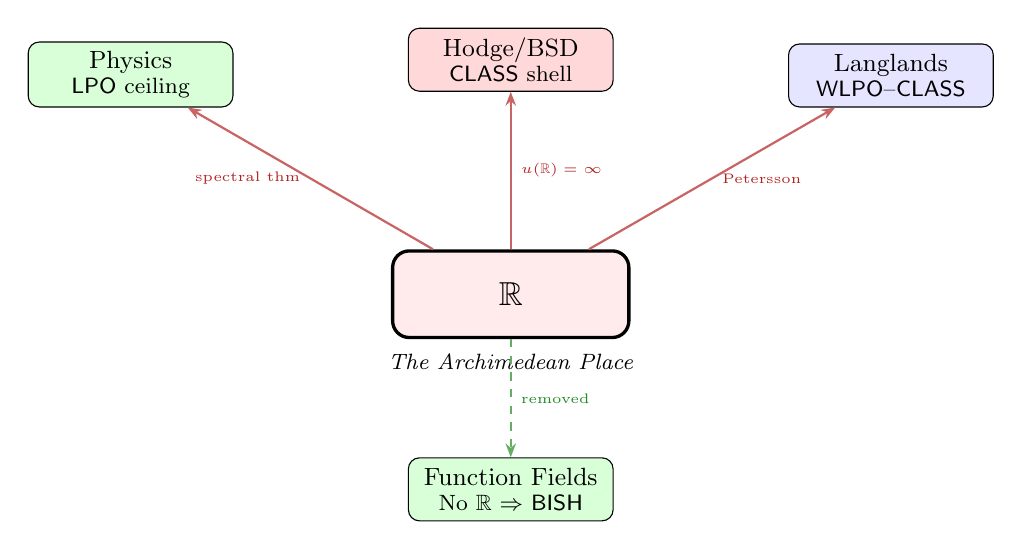
\begin{tikzpicture}[scale=0.85]
  % The real line as source
  \node[draw, very thick, rounded corners=6pt, fill=red!8,
        minimum width=3cm, minimum height=1.1cm,
        font=\large\bfseries\sffamily] (R) {$\mathbb{R}$};
  \node[below=2pt of R, font=\footnotesize\itshape] {The Archimedean Place};

  % Three domains
  \node[bishbox, minimum width=2.6cm, above left=1.8cm and 2cm of R] (phys)
    {Physics\\[-2pt]{\footnotesize\LPO{} ceiling}};
  \node[classbox, minimum width=2.6cm, above=2cm of R] (hodge)
    {Hodge/BSD\\[-2pt]{\footnotesize \CLASS{} shell}};
  \node[bridgebox, minimum width=2.6cm, above right=1.8cm and 2cm of R] (lang)
    {Langlands\\[-2pt]{\footnotesize \WLPO--\CLASS}};

  % Arrows from R
  \draw[arr, classred!70] (R) -- (phys)
    node[midway, left, font=\tiny, text=classred] {spectral thm};
  \draw[arr, classred!70] (R) -- (hodge)
    node[midway, right, font=\tiny, text=classred] {$u(\mathbb{R})=\infty$};
  \draw[arr, classred!70] (R) -- (lang)
    node[midway, right, font=\tiny, text=classred] {Petersson};

  % Function field (no R)
  \node[bishbox, minimum width=2.6cm, below=1.5cm of R] (ff)
    {Function Fields\\[-2pt]{\footnotesize No $\mathbb{R}$ $\Rightarrow$ \BISH}};
  \draw[arr, bishgreen!70, dashed] (R) -- (ff)
    node[midway, right, font=\tiny, text=bishgreen] {removed};
\end{tikzpicture}

\vfill
{\footnotesize Constructive Reverse Mathematics Series\\
Papers 1--98\quad$\cdot$\quad 96,200+ lines Lean~4\quad$\cdot$\quad Zero \texttt{sorry}\\[4pt]
Series DOI: \href{https://doi.org/10.5281/zenodo.17054050}{10.5281/zenodo.17054050}\par}
\end{titlepage}

%── Dedication ────────────────────────────────────────────
\clearpage
\thispagestyle{empty}
\vspace*{\fill}
\begin{center}
\textit{To Mimi}
\end{center}
\vspace*{\fill}

%── Epigraph ──────────────────────────────────────────────
\clearpage
\thispagestyle{empty}
\vspace*{\fill}
\begin{center}
{\large
\foreignlanguage{greek}{%
>En >arq\~h| \~hn <o L'ogos,\\[4pt]
ka`i <o L'ogos \~hn pr`os t`on Je'on,\\[4pt]
ka`i Je`os \~hn <o L'ogos.%
}}
\end{center}
\vspace{1cm}
\begin{center}
\normalsize\textit{In the beginning was the Word,\\
and the Word was with God,\\
and the Word was God.}\\[6pt]
--- John 1:1
\end{center}
\vspace*{\fill}

%── Table of Contents ─────────────────────────────────────
\tableofcontents
\clearpage

%══════════════════════════════════════════════════════════
% PREFACE
%══════════════════════════════════════════════════════════
\chapter*{Preface: The Map and the Territory}
\addcontentsline{toc}{chapter}{Preface}
\markboth{Preface}{Preface}

In 1967, Errett Bishop published \emph{Foundations of Constructive Analysis} and defined a program: rebuild mathematics so that every existence claim comes with an explicit witness, every function is computable, every proof provides an algorithm. Over the next three decades, Bishop and his successors---Bridges, Richman, Ishihara, Bauer---mapped the precise hierarchy of non-constructive principles that separate different strengths of mathematical reasoning. They called these the \emph{omniscience principles}, and the cartography they produced was meticulous, rigorous, and almost entirely ignored.

Constructive mathematics received recognition at the highest levels---Bauer's 2017 address to the AMS, for instance---but produced no foundational change in practice. The mainstream continued to use classical logic without asking what it cost. The hierarchy Bishop built remained a curiosity of mathematical philosophy, not a tool for working mathematicians or scientists.

The missing step was not advocacy but \emph{measurement}. Nobody had taken the actual theorems of physics and pure mathematics---the ones that produce numbers, predict experiments, settle conjectures---and calibrated them against Bishop's hierarchy. This monograph reports the results of that calibration: 98 papers, 96,200 lines of machine-checked Lean~4 code, spanning quantum mechanics, general relativity, the Hodge conjecture, the Birch and Swinnerton-Dyer conjecture, and the Langlands program, all asking a single question:

\begin{thesisbox}[Central Question]
\textbf{What logical resources does this theorem actually need?}
\end{thesisbox}

Not ``is it true?'' but ``what do you have to believe to prove it?''
Not ``how complex is the proof?'' but ``which non-negotiable principles does the proof depend on?''

The answer is this:

\begin{thesisbox}[Central Finding]
\textbf{The logical cost of mathematics is the logical cost of the real numbers.}
\end{thesisbox}

Every non-constructive principle that mathematics requires enters through one object: the real number line~$\mathbb{R}$. Remove it, and both physics and the deepest arithmetic geometry collapse to fully constructive mathematics---mathematics where every ``there exists'' comes with an explicit witness, every algorithm terminates with a known bound, every claim can be checked by a machine.

This monograph explains that finding, the 98-paper journey that established it, and why it matters for anyone who builds systems, reasons about structure, or wants to understand what makes hard problems hard.

\subsection*{How to Read This Document}

\textbf{You do not need algebraic geometry to read this monograph.} Every technical term is defined before it is used; every hard concept gets an analogy first. If you have a background in linear algebra and multivariable calculus, Chapter~1 will give you everything else.

\textbf{Chapter~1} builds the complete conceptual toolkit. Every technical term is defined here before it appears elsewhere.
\textbf{Chapters~2--3} establish the mathematical foundation: the five great conjectures and the DPT axioms.
\textbf{Chapters~4--7} are the core: the Squeeze protocol, the Hodge campaign, the BSD application, and the motivic architecture that explains why the pattern holds.
\textbf{Chapters~8--9} draw cross-domain implications and conclude.
\textbf{Appendices} provide the complete paper list, glossary, and hierarchy.

Every claim links to the original paper. No formal proof is required to follow the argument. Diagrams and analogies carry the load.


%══════════════════════════════════════════════════════════
% CHAPTER 1
%══════════════════════════════════════════════════════════
\chapter{The Measuring Instrument}

This chapter builds everything you need before the mathematics starts. No concept is skipped. By the end, you will understand the hierarchy, what an oracle is, why the real numbers are special, and what formal verification means.

%── 1.1 ───────────────────────────────────────────────────
\section{What ``Exists'' Costs}

When a physicist says ``there exists a ground state energy for this Hamiltonian,'' they mean something very specific: given enough compute time, you can find it. The eigenvalue is computable. You can write an algorithm that produces it to any desired precision. The physicist's ``exists'' comes with a recipe.

When a number theorist says ``there exists a rational point on this elliptic curve,'' they may mean something entirely different. They may have proved the point exists by contradiction---by showing that its non-existence leads to an absurdity. But they cannot tell you what the point is, how to find it, or how long the search would take. Their ``exists'' is a logical guarantee with no recipe attached.

These two kinds of ``exists'' have different logical costs. The physicist's version is cheap. The number theorist's version may be expensive. \textbf{Constructive Reverse Mathematics (CRM)} is the framework that makes this difference precise.

\begin{thesisbox}[The CRM Question]
For a given theorem, what is the minimum set of logical principles needed to prove it?
Can you do it with just algorithms and explicit witnesses?
Or do you need an \emph{oracle}---a hypothetical device that answers questions no algorithm can?
\end{thesisbox}


%── 1.2 ───────────────────────────────────────────────────
\section{Constructive Reverse Mathematics}

``Reverse mathematics'' inverts the usual direction of mathematical reasoning. Normally, you start with axioms and derive theorems. Reverse mathematics starts with theorems and asks: \emph{which axioms did you actually need?}

Think of it as a dependency audit for mathematical proofs. A software project has a dependency tree---libraries it imports, APIs it calls. Some dependencies are load-bearing (remove them and the code breaks). Others are convenience (you could replace them with a few lines). CRM is \texttt{npm audit} for mathematical proofs: it traces every logical dependency, flags which are structural and which are scaffolding, and reports the minimum viable dependency set.

\begin{thesisbox}[Formal Definition]
\textbf{CRM classification} of a theorem $T$: identify the weakest principle $P$ in the hierarchy (\BISH{} $\subset$ \MP{} $\subset$ \LLPO{} $\subset$ \WLPO{} $\subset$ \LPO{} $\subset$ \CLASS) such that $T$ is provable in \BISH{} + $P$. The classification is \emph{tight} if additionally $T$ implies $P$ over \BISH{} (reverse direction). When both directions hold ($T \Leftrightarrow P$ over \BISH), the classification is \emph{biconditional}.
\end{thesisbox}

The CRM program (\paperref{1--98}) performed this audit on theorems across all of mathematical physics (\paperref{1--44}) and arithmetic geometry (\paperref{45--98}). The result: a uniform classification of where logical difficulty lives and why.


%── 1.3 ───────────────────────────────────────────────────
\section{The Hierarchy}

Every theorem lives somewhere on a hierarchy of logical strength. Figure~\ref{fig:hierarchy} shows the complete hierarchy from weakest (cheapest) to strongest (most expensive).

\begin{figure}[htbp]
\centering
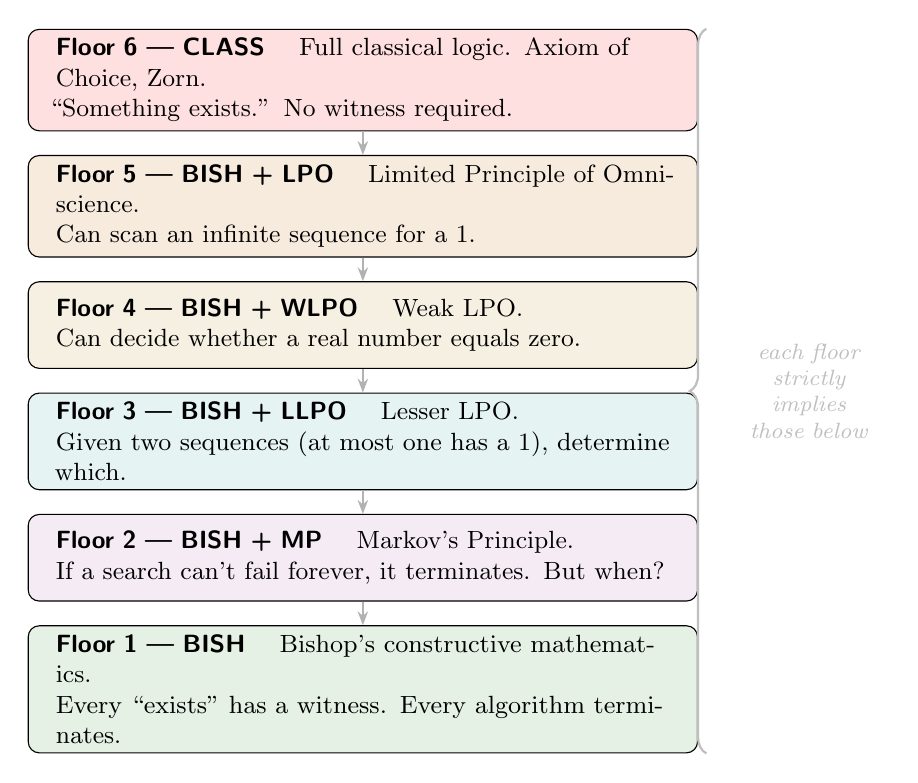
\begin{tikzpicture}[
  floor/.style={
    draw, rounded corners=4pt,
    minimum width=8.5cm, minimum height=1.1cm,
    align=left, font=\small,
    text width=7.8cm
  },
  node distance=0.3cm
]
  % Floor 6
  \node[floor, fill=red!12] (f6) {
    \textbf{\textsf{Floor 6 --- \CLASS}}
    \quad Full classical logic. Axiom of Choice, Zorn.\\
    ``Something exists.'' No witness required.
  };
  % Floor 5
  \node[floor, fill=lpoamber!15, below=of f6] (f5) {
    \textbf{\textsf{Floor 5 --- \BISH{} + \LPO}}
    \quad Limited Principle of Omniscience.\\
    Can scan an infinite sequence for a~1.
  };
  % Floor 4
  \node[floor, fill=wlpogold!12, below=of f5] (f4) {
    \textbf{\textsf{Floor 4 --- \BISH{} + \WLPO}}
    \quad Weak LPO.\\
    Can decide whether a real number equals zero.
  };
  % Floor 3
  \node[floor, fill=llpocyan!10, below=of f4] (f3) {
    \textbf{\textsf{Floor 3 --- \BISH{} + \LLPO}}
    \quad Lesser LPO.\\
    Given two sequences (at most one has a~1), determine which.
  };
  % Floor 2
  \node[floor, fill=mppurple!8, below=of f3] (f2) {
    \textbf{\textsf{Floor 2 --- \BISH{} + \MP}}
    \quad Markov's Principle.\\
    If a search can't fail forever, it terminates. But when?
  };
  % Floor 1
  \node[floor, fill=bishgreen!12, below=of f2] (f1) {
    \textbf{\textsf{Floor 1 --- \BISH}}
    \quad Bishop's constructive mathematics.\\
    Every ``exists'' has a witness. Every algorithm terminates.
  };

  % Arrows
  \foreach \a/\b in {f6/f5, f5/f4, f4/f3, f3/f2, f2/f1} {
    \draw[arr, gray!60] (\a.south) -- (\b.north);
  }

  % Implication label
  \draw[decorate, decoration={brace, amplitude=6pt, mirror},
        thick, gray!50]
    ([xshift=3pt]f6.north east) -- ([xshift=3pt]f1.south east)
    node[midway, right=8pt, font=\footnotesize\itshape, text width=1.8cm,
         align=center] {each floor\\strictly\\implies\\those below};
\end{tikzpicture}
\caption{The CRM hierarchy. Each floor strictly implies those below it. The program's central finding: most of mathematics lives on Floor~1 (\BISH). Almost everything on higher floors got there via one object: $\mathbb{R}$.}
\label{fig:hierarchy}
\end{figure}

\begin{analogybox}[Analogy: The Restaurant Menu]
\begin{itemize}
  \item \textbf{\BISH:} The dish is on the menu with a recipe and a prep time. You can make it.
  \item \textbf{\MP:} The dish is on the menu. The recipe terminates, but you don't know when the timer goes off. You wait, knowing it will come---eventually.
  \item \textbf{\LLPO:} Two ovens, at most one is on. You can determine which---but only by committing to check one first.
  \item \textbf{\WLPO:} A soup is simmering. You must decide: is the salt content \emph{exactly} zero, or is it nonzero? After a million tastings, you still can't be sure---the salt might be $10^{-100}$.
  \item \textbf{\LPO:} An infinite buffet line. Somewhere, one dish has a cherry on top. You must scan every plate.
  \item \textbf{\CLASS:} The chef says ``trust me, something delicious exists,'' and you take his word without seeing the kitchen.
\end{itemize}
\end{analogybox}


%── 1.4 ───────────────────────────────────────────────────
\section{What an Oracle Is}

In this framework, an ``oracle'' is a hypothetical device that answers a question no algorithm can answer in finite time. It is not mystical---it is a precise specification of computational power. Figure~\ref{fig:oracles} compares the three main oracles.

\begin{figure}[htbp]
\centering
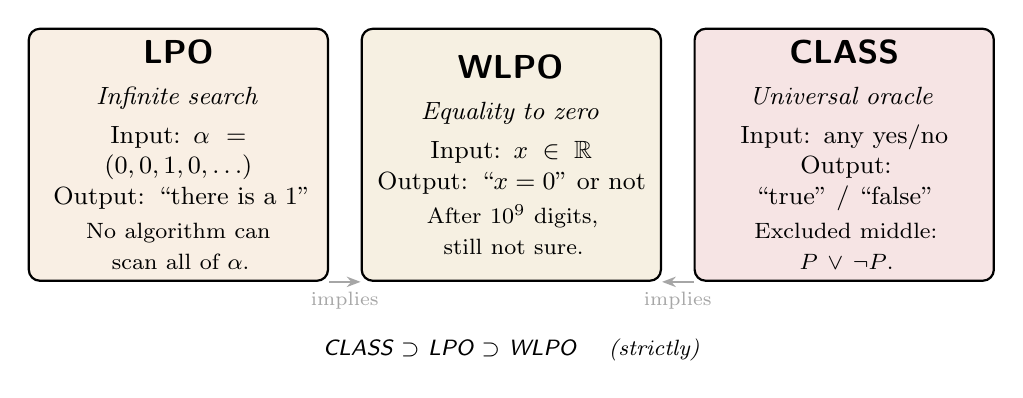
\begin{tikzpicture}[
  obox/.style={draw, rounded corners=4pt, thick,
    minimum width=3.8cm, minimum height=3.2cm,
    align=center, font=\small, text width=3.4cm},
  node distance=0.4cm
]
  % LPO
  \node[obox, fill=lpoamber!12] (lpo) {
    \textbf{\large\LPO}\\[4pt]
    \textit{Infinite search}\\[3pt]
    Input: $\alpha = (0,0,1,0,\ldots)$\\
    Output: ``there is a~1''\\[3pt]
    {\footnotesize No algorithm can\\scan all of $\alpha$.}
  };
  % WLPO
  \node[obox, fill=wlpogold!12, right=of lpo] (wlpo) {
    \textbf{\large\WLPO}\\[4pt]
    \textit{Equality to zero}\\[3pt]
    Input: $x \in \mathbb{R}$\\
    Output: ``$x = 0$'' or not\\[3pt]
    {\footnotesize After $10^9$ digits,\\still not sure.}
  };
  % CLASS
  \node[obox, fill=classred!12, right=of wlpo] (class) {
    \textbf{\large\CLASS}\\[4pt]
    \textit{Universal oracle}\\[3pt]
    Input: any yes/no\\
    Output: ``true'' / ``false''\\[3pt]
    {\footnotesize Excluded middle:\\$P \vee \neg P$.}
  };

  % Arrows showing strength
  \draw[arr, thick, gray!70] (class.south west) -- (wlpo.south east)
    node[midway, below, font=\scriptsize] {implies};
  \draw[arr, thick, gray!70] (lpo.south east) -- (wlpo.south west)
    node[midway, below, font=\scriptsize] {implies};

  % Strength label
  \node[below=0.6cm of wlpo, font=\footnotesize\itshape] {%
    \CLASS{} $\supset$ \LPO{} $\supset$ \WLPO{}
    \quad (strictly)};
\end{tikzpicture}
\caption{The three main oracles. Each answers a question no algorithm can answer in finite time. \CLASS{} is the most powerful; \WLPO{} the weakest (tests equality to zero). The CRM question: \emph{which oracle does your proof need?}}
\label{fig:oracles}
\end{figure}

When CRM says a theorem ``costs \LPO,'' it means: you cannot prove this theorem without the ability to scan infinite sequences. When it says ``\BISH,'' it means: no oracle needed---an algorithm suffices.

\textbf{The key intuition:} each oracle is a weaker version of the one above it. \CLASS{} can answer \emph{any} yes/no question. \LPO{} can only answer ``is there a 1 somewhere in this infinite list?'' \WLPO{} can only answer ``is this real number exactly zero?'' \LLPO{} can only answer ``given two lists where at most one has a 1, which one?'' Each step down shrinks the oracle's power---and CRM asks: what is the \emph{weakest} oracle your proof actually needs?


%── 1.5 ───────────────────────────────────────────────────
\section{The Archimedean Place and Why $\mathbb{R}$ Is the Source of All Difficulty}

This is the core of the entire program. Understand this section and you understand the finding.

\textbf{The rationals are decidable.} Every question about rational numbers has an algorithmic answer. Is $3/7 < 5/11$? Multiply out and compare: $33$ vs.\ $35$. Done. \BISH. The rational numbers are computationally tame.

\textbf{The reals are not.} A real number is typically represented as an infinite Cauchy sequence of rationals. To test whether two reals are equal, you must (in principle) compare infinitely many terms. This requires \WLPO. To search a sequence of reals for one with a particular property requires \LPO. The real numbers are computationally wild.

The mathematical term for where the real numbers sit is the \textbf{Archimedean place}---the completion of $\mathbb{Q}$ at infinity, as opposed to the $p$-adic completions at finite primes. The program's finding is that this one place---the Archimedean place, i.e., the real number line---is the sole source of non-constructive content in all of mathematics.

\textbf{Why does $\mathbb{R}$ force non-constructive principles?} The technical reason is captured by an invariant called $u(\mathbb{R}) = \infty$. The \textbf{$u$-invariant} of a field $F$ measures the largest dimension~$n$ in which every quadratic form over $F$ of dimension~$n$ has a nontrivial zero. For the reals, consider the sum of squares $x_1^2 + x_2^2 + \cdots + x_n^2$: every term is non-negative, so the sum is zero only when every $x_i$ is zero. This works for \emph{every}~$n$---the form $x_1^2 + \cdots + x_n^2$ over $\mathbb{R}$ never has a nontrivial zero, no matter how many variables you add. Hence $u(\mathbb{R}) = \infty$. By contrast, over a $p$-adic field $\mathbb{Q}_p$ this fails for $n \geq 5$ (a theorem of Springer): $u(\mathbb{Q}_p) = 4$.

What does this have to do with constructivity? Positive-definite forms give you \emph{inner products}: $\langle x, y \rangle = \sum x_i y_i$ is positive-definite over~$\mathbb{R}$. Inner products give you \emph{projections} (decomposing vectors into components), \emph{norms} (measuring distances), and \emph{heights} (measuring arithmetic complexity). These are the tools of analysis. But using them requires \emph{deciding properties of real numbers}---is this inner product zero? is this norm smaller than that one?---and those decisions cost oracles (\WLPO{} for equality, \LPO{} for search).

The chain is: $u(\mathbb{R}) = \infty \;\Rightarrow\;$ positive-definite forms exist in all dimensions $\;\Rightarrow\;$ inner products, norms, heights $\;\Rightarrow\;$ decisions about real numbers $\;\Rightarrow\;$ oracles (\WLPO/\LPO/\CLASS).

Three fields independently exploit this same mechanism. Each one uses a positive-definite form enabled by $\mathbb{R}$:
\begin{itemize}
  \item \textbf{Hilbert space inner product} (physics): the inner product $\langle \psi | \phi \rangle$ on quantum states. Used for spectral decomposition. You already know this from linear algebra.
  \item \textbf{Rosati involution} (arithmetic geometry): a positive-definite pairing on algebraic cycles, analogous to an inner product. It gives heights their finiteness properties (the Northcott property). Explained in detail in \S\ref{sec:flt} and Chapter~3.
  \item \textbf{Petersson inner product} (automorphic forms): an $L^2$ inner product on a space of modular forms, used to decompose them into eigenforms. Explained in the modular forms subsection below and Chapter~5.
\end{itemize}

\noindent All three structures exist because $u(\mathbb{R}) = \infty$. Remove $\mathbb{R}$ from the picture (as happens in function fields), and none of them are available---everything is \BISH.

\begin{figure}[htbp]
\centering
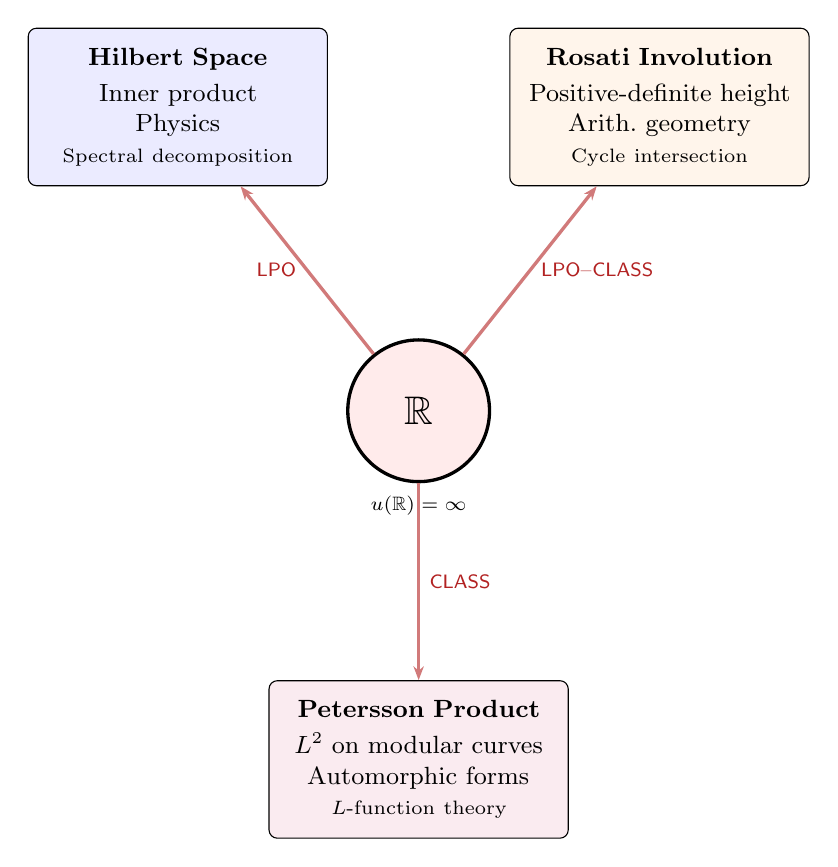
\begin{tikzpicture}[
  block/.style={draw, rounded corners=3pt,
    minimum width=3.8cm, minimum height=2cm,
    align=center, font=\small, text width=3.5cm}
]
  % Central R
  \node[draw, very thick, circle, fill=red!8,
        minimum size=1.8cm, font=\Large\bfseries] (R) {$\mathbb{R}$};
  \node[below=1pt of R, font=\scriptsize\itshape] (Rsub)
    {$u(\mathbb{R}) = \infty$};

  % Three structures
  \node[block, fill=blue!8, above left=2.2cm and 0.5cm of R] (hilbert) {
    \textbf{Hilbert Space}\\[2pt]
    Inner product\\
    Physics\\
    {\scriptsize Spectral decomposition}
  };
  \node[block, fill=orange!8, above right=2.2cm and 0.5cm of R] (rosati) {
    \textbf{Rosati Involution}\\[2pt]
    Positive-definite height\\
    Arith.\ geometry\\
    {\scriptsize Cycle intersection}
  };
  \node[block, fill=purple!8, below=2.5cm of R] (petersson) {
    \textbf{Petersson Product}\\[2pt]
    $L^2$ on modular curves\\
    Automorphic forms\\
    {\scriptsize $L$-function theory}
  };

  % Arrows
  \draw[arr, very thick, classred!60] (R) -- (hilbert)
    node[midway, left, font=\scriptsize, text=classred]
      {\LPO};
  \draw[arr, very thick, classred!60] (R) -- (rosati)
    node[midway, right, font=\scriptsize, text=classred]
      {\LPO--\CLASS};
  \draw[arr, very thick, classred!60] (R) -- (petersson)
    node[midway, right, font=\scriptsize, text=classred]
      {\CLASS};
\end{tikzpicture}
\caption{$\mathbb{R}$ as the sole source of non-constructive content. Each arrow carries the logical cost of the positive-definite structure it enables.}
\label{fig:archimedean-source}
\end{figure}


\begin{analogybox}[Analogy: The Power Plant]
Imagine mathematics as a city. The entire city runs on electricity (logical principles). CRM traced every wire and found they all lead back to one power plant: the real number line. Some neighborhoods (physics) draw moderate power (\LPO). Others (number theory) draw heavy power (\CLASS). But the plant is the same. Shut it down, and the city goes dark. Build a different city without $\mathbb{R}$ (function fields, for instance), and no power plant is needed---everything runs on local generators (\BISH).
\end{analogybox}

\begin{keyrefbox}
\textbf{Key references:} \paperref{70} (The Archimedean Principle---capstone) formalizes the four-domain partition. \paperref{35} and \paperref{40} establish the physics ceiling.
\end{keyrefbox}


%── 1.6 ───────────────────────────────────────────────────
\section{Projection vs.\ Search}

Why is physics logically cheaper than number theory? Both use the real numbers. Both pay the Archimedean toll. But they use $\mathbb{R}$ differently. Figure~\ref{fig:proj-search} illustrates the structural distinction.

\begin{figure}[htbp]
\centering
\resizebox{\textwidth}{!}{%
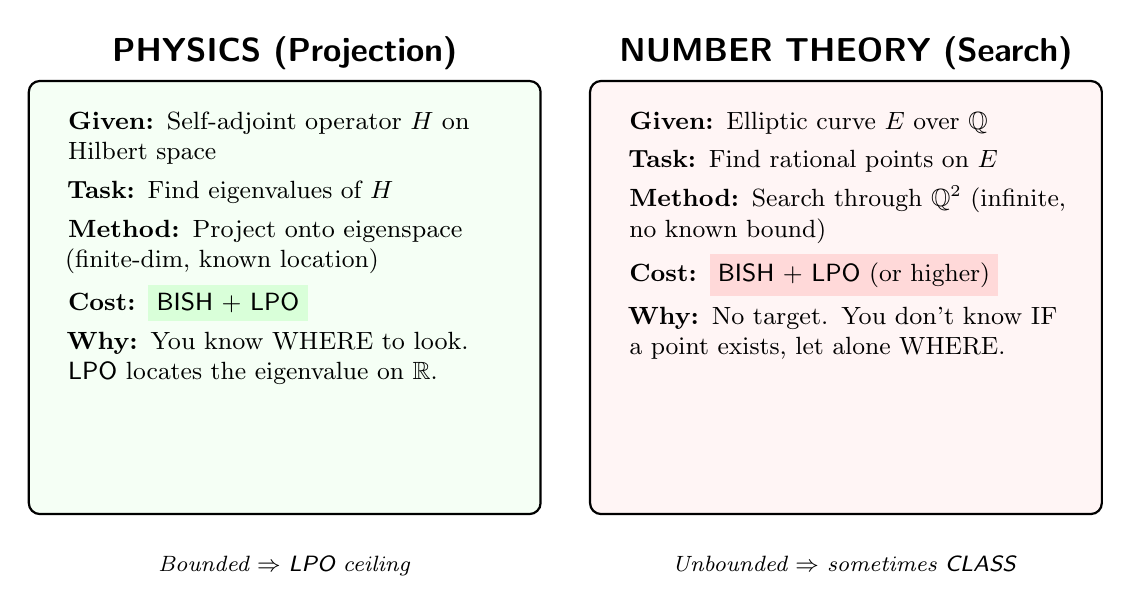
\begin{tikzpicture}[
  panel/.style={draw, rounded corners=4pt, thick,
    minimum width=6.5cm, minimum height=5.5cm,
    align=center, text width=6cm},
  paneltext/.style={font=\small, align=left, text width=5.5cm}
]
  % Physics panel
  \node[panel, fill=green!4] (phys) {};
  \node[above=0pt of phys.north, font=\large\bfseries\sffamily,
        anchor=south] {PHYSICS (Projection)};

  \node[paneltext, below=8pt of phys.north, anchor=north] {
    \textbf{Given:} Self-adjoint operator $H$ on Hilbert space\\[3pt]
    \textbf{Task:} Find eigenvalues of $H$\\[3pt]
    \textbf{Method:} Project onto eigenspace
    (finite-dim, known location)\\[3pt]
    \textbf{Cost:} \colorbox{green!15}{\BISH{} + \LPO}\\[3pt]
    \textbf{Why:} You know WHERE to look.
    \LPO{} locates the eigenvalue on $\mathbb{R}$.
  };

  % Number theory panel
  \node[panel, fill=red!4, right=0.6cm of phys] (nt) {};
  \node[above=0pt of nt.north, font=\large\bfseries\sffamily,
        anchor=south] {NUMBER THEORY (Search)};

  \node[paneltext, below=8pt of nt.north, anchor=north] {
    \textbf{Given:} Elliptic curve $E$ over $\mathbb{Q}$\\[3pt]
    \textbf{Task:} Find rational points on $E$\\[3pt]
    \textbf{Method:} Search through $\mathbb{Q}^2$
    (infinite, no known bound)\\[3pt]
    \textbf{Cost:} \colorbox{red!15}{\BISH{} + \LPO{} (or higher)}\\[3pt]
    \textbf{Why:} No target. You don't know IF
    a point exists, let alone WHERE.
  };

  % Bottom comparison
  \node[below=0.4cm of phys.south, font=\footnotesize\itshape,
        text width=6cm, align=center]
    {Bounded $\Rightarrow$ \LPO{} ceiling};
  \node[below=0.4cm of nt.south, font=\footnotesize\itshape,
        text width=6cm, align=center]
    {Unbounded $\Rightarrow$ sometimes \CLASS};
\end{tikzpicture}%
}
\caption{Projection is bounded (known target subspace); search is unbounded (no target). This structural difference explains why physics tops out at \BISH{} + \LPO{} while number theory sometimes needs \CLASS. Both start from $\mathbb{R}$, but physics uses $\mathbb{R}$ to project, while number theory uses $\mathbb{R}$ to search.}
\label{fig:proj-search}
\end{figure}


%── 1.7 ───────────────────────────────────────────────────
\section{The Physics Ceiling}

\paperref{1--44} systematically calibrated every major physical theory against the hierarchy. Table~\ref{tab:physics-ceiling} shows the result. Two axioms that appear in some physics proofs---the Fan Theorem (\FT) and Dependent Choice (\DC)---are shown to be \textbf{dispensable} (\paperref{30--31}). The \textbf{Fan Theorem} says: every function from Cantor space $\{0,1\}^\mathbb{N}$ to $\mathbb{N}$ that is pointwise continuous is \emph{uniformly} continuous. \textbf{Dependent Choice} says: given a relation $R$ on a set $A$ where every element has a successor, you can build an infinite chain. Both are logically independent of the main hierarchy and neither is required for any physical theory.

\begin{table}[htbp]
\centering\small
\caption{Physics calibration results. Every physical theory was audited for its CRM cost. The ceiling is \BISH{} + \LPO, entering through the spectral theorem for unbounded operators on $\mathbb{R}$.}
\label{tab:physics-ceiling}
\renewcommand{\arraystretch}{1.2}
\begin{tabular}{@{}l l l@{}}
\toprule
\textbf{Domain} & \textbf{Theorem / Concept} & \textbf{CRM Cost} \\
\midrule
\rowcolor{green!6}
Classical Mechanics & Newton, Lagrange, Hamilton & \BISH \\
\rowcolor{green!6}
Quantum Mechanics & Schr\"odinger equation & \BISH \\
\rowcolor{green!6}
 & Heisenberg uncertainty (\paperref{6}) & \BISH \\
\rowcolor{lpoamber!8}
 & Born rule (\paperref{16}) & \BISH{} + \LPO \\
\rowcolor{lpoamber!8}
 & Spectral theorem & \BISH{} + \LPO \\
\rowcolor{green!6}
 & CHSH / Tsirelson bound (\paperref{11}) & \BISH \\
\rowcolor{green!6}
General Relativity & Schwarzschild interior (\paperref{5}) & \BISH \\
\rowcolor{lpoamber!8}
 & Singularity / event horizon & \BISH{} + \LPO \\
\rowcolor{lpoamber!8}
Statistical Mechanics & 1D Ising model (\paperref{8--9}) & \BISH{} + \LPO \\
\rowcolor{green!6}
QFT & QED renormalization (\paperref{32}) & \BISH \\
\rowcolor{lpoamber!8}
 & QCD confinement (\paperref{33}) & \BISH{} + \LPO \\
\rowcolor{green!6}
 & Scattering amplitudes (\paperref{34}) & \BISH \\
\rowcolor{llpocyan!6}
Quantum Information & Bell nonlocality (\paperref{21}) & \BISH{} + \LLPO \\
\rowcolor{wlpogold!6}
 & Decoherence (\paperref{14}) & \BISH{} + \WLPO \\
\midrule
\multicolumn{2}{@{}l}{\textbf{Ceiling:}} & \textbf{\BISH{} + \LPO} \\
\bottomrule
\end{tabular}
\end{table}

\textbf{The metatheorem (\paperref{35, 40}):} \BISH{} + \LPO{} is the complete logical constitution of empirically accessible physics. No physical prediction requires more than \LPO. This is a ceiling, not a floor---individual theories may need less.

A striking corollary of the physics ceiling: the ``measurement problem'' --- the century-old debate over what happens when a quantum system is observed --- dissolves under CRM. \paperref{44} showed that different quantum interpretations have different CRM costs: Copenhagen = \BISH{} + \LPO, Many-Worlds = \BISH{} + \LPO, Bohmian = \BISH{} + \MP. They are logically distinct but empirically equivalent.


%── 1.8 ───────────────────────────────────────────────────
\section{Formal Verification in Lean 4}

Every claim in this program is machine-checked. The proof assistant Lean~4, built on a small trusted kernel and a large mathematical library (Mathlib), verifies every logical step.

\begin{figure}[htbp]
\centering
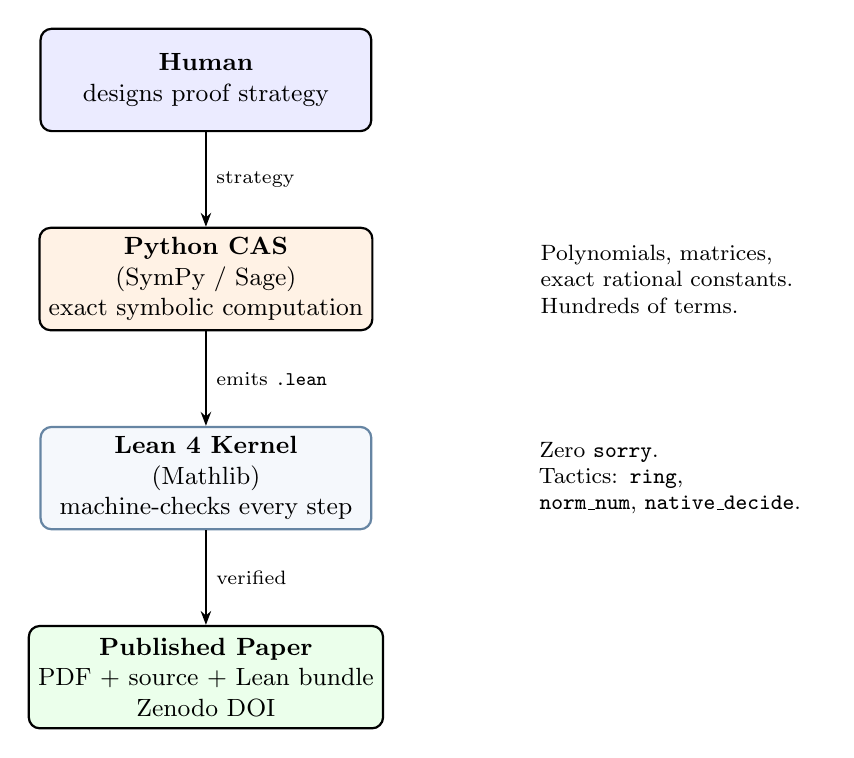
\begin{tikzpicture}[
  stage/.style={draw, rounded corners=4pt, thick,
    minimum width=4.2cm, minimum height=1.3cm,
    align=center, font=\small},
  node distance=1.2cm
]
  \node[stage, fill=blue!8] (human)
    {\textbf{Human}\\designs proof strategy};
  \node[stage, fill=orange!10, below=of human] (cas)
    {\textbf{Python CAS}\\(SymPy / Sage)\\exact symbolic computation};
  \node[stage, fill=leanbg, draw=leanblue!60, below=of cas] (lean)
    {\textbf{Lean 4 Kernel}\\(Mathlib)\\machine-checks every step};
  \node[stage, fill=green!8, below=of lean] (pub)
    {\textbf{Published Paper}\\PDF + source + Lean bundle\\Zenodo DOI};

  \draw[arr] (human) -- (cas)
    node[midway, right, font=\scriptsize] {strategy};
  \draw[arr] (cas) -- (lean)
    node[midway, right, font=\scriptsize] {emits \texttt{.lean}};
  \draw[arr] (lean) -- (pub)
    node[midway, right, font=\scriptsize] {verified};

  % Annotations
  \node[right=2cm of cas, font=\footnotesize, text width=3.5cm, align=left]
    {Polynomials, matrices,\\exact rational constants.\\Hundreds of terms.};
  \node[right=2cm of lean, font=\footnotesize, text width=3.5cm, align=left]
    {Zero \texttt{sorry}.\\Tactics: \texttt{ring},\\
     \texttt{norm\_num}, \texttt{native\_decide}.};
\end{tikzpicture}
\caption{The asymmetric offloading pipeline. Humans design strategy; Python CAS computes exact algebra; Lean~4 verifies. Development time dropped from 4 months (\paperref{5}, manual) to 1 hour (\paperref{77}, pipelined) for comparable proof density---a 2,900$\times$ speedup.}
\label{fig:pipeline}
\end{figure}

\textbf{Zero-sorry policy:} In Lean, \texttt{sorry} is a keyword that means ``I'm skipping this proof---trust me.'' The program has zero instances of \texttt{sorry} across 96,200+ lines. Every step is verified.

\begin{analogybox}[Analogy: Double-Entry Bookkeeping]
Lean~4 is to mathematics what double-entry bookkeeping is to accounting. Every debit must have a credit. Every claim must have a proof term. The computer is the auditor that never sleeps, never gets tired, and never lets a balance error pass.
\end{analogybox}

%── 1.9 ───────────────────────────────────────────────────
\section{The Algebraic Geometry Toolkit (A Primer)}

The rest of this monograph uses concepts from algebraic geometry and number theory. This section defines everything you need, starting from examples. \textbf{Read this section first.} Every jargon term in Chapters 2--7 is introduced here.

\subsection*{Varieties: Shapes Defined by Polynomials}

An \textbf{algebraic variety} is a shape defined by polynomial equations. A circle ($x^2 + y^2 = 1$) is a variety. A line ($y = 2x + 3$) is a variety. An \textbf{elliptic curve} like $y^2 + y = x^3 - x$ is a variety---a smooth cubic in the plane, shaped like a doughnut.

``\textbf{Smooth}'' means no sharp corners or self-intersections. ``\textbf{Projective}'' means we work in a setting where parallel lines meet at infinity (adding ``points at infinity'' to close up the shape). A ``smooth projective variety'' is just a nice closed shape defined by polynomials, living in projective space.

\textbf{Rational points} are solutions with \emph{rational} coordinates. The circle $x^2 + y^2 = 1$ has rational points like $(3/5, 4/5)$. The elliptic curve $y^2 + y = x^3 - x$ has the rational point $(0, 0)$. Finding all rational points is the central problem of number theory.

\subsection*{Cohomology: Counting Holes}

You already know that a circle has one ``hole'' (you can lasso it with a loop), a torus has two independent holes (one around the tube, one through the tube), and a sphere has no holes in the loop sense but encloses a cavity.

\textbf{Cohomology} makes this precise. It assigns a vector space $H^k(X)$ to each variety $X$ and each dimension $k$. Why a vector space and not just a number? Because the vector space remembers \emph{how} the holes are related to each other, not just how many there are. (The number of independent holes is the \emph{dimension} of the vector space.)
\begin{itemize}
  \item $H^0$ counts connected components.
  \item $H^1$ counts independent 1-dimensional holes (loops that don't bound disks).
  \item $H^2$ counts 2-dimensional cavities (surfaces that don't bound solids).
  \item $H^k$ counts $k$-dimensional ``holes.'' (For $k \geq 3$, geometric intuition fades, but the algebra continues to work perfectly.)
\end{itemize}

For a torus: $H^0 = \mathbb{Q}$ (one piece), $H^1 = \mathbb{Q}^2$ (two independent loops), $H^2 = \mathbb{Q}$ (one cavity).

Here is the key fact for this monograph, and it is remarkable: there are \emph{several completely different methods} to compute these vector spaces---different ``flavours'' of cohomology. You can count holes topologically (triangulate the shape and count faces), or algebraically (study polynomial differential forms), or arithmetically (watch how symmetries of number fields act on the shape). All methods give vector spaces of the same dimension. But they are computed by entirely different techniques and---crucially---they have different \emph{logical costs}:

\begin{figure}[htbp]
\centering
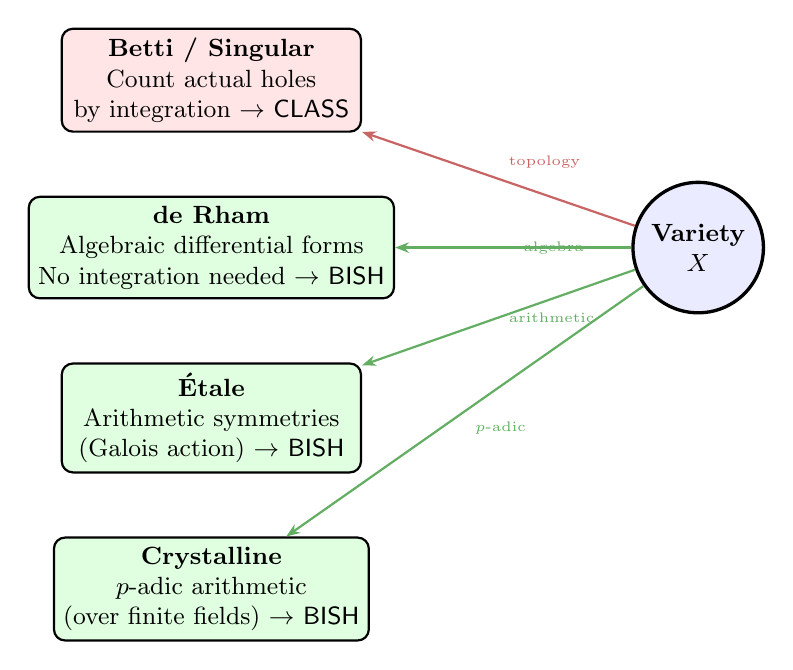
\begin{tikzpicture}[
  coh/.style={draw, rounded corners=4pt, thick,
    minimum width=3.8cm, minimum height=1.1cm,
    align=center, font=\small},
  node distance=0.5cm
]
  \node[coh, fill=red!10] (betti)
    {\textbf{Betti / Singular}\\Count actual holes\\by integration $\to$ \CLASS};
  \node[coh, fill=green!12, below=0.8cm of betti] (dr)
    {\textbf{de Rham}\\Algebraic differential forms\\No integration needed $\to$ \BISH};
  \node[coh, fill=green!12, below=0.8cm of dr] (et)
    {\textbf{\'Etale}\\Arithmetic symmetries\\ (Galois action) $\to$ \BISH};
  \node[coh, fill=green!12, below=0.8cm of et] (crys)
    {\textbf{Crystalline}\\$p$-adic arithmetic\\(over finite fields) $\to$ \BISH};

  % Arrows to the shape
  \node[right=3cm of dr, draw, very thick, circle, fill=blue!8,
        minimum size=1.5cm, font=\small\bfseries, align=center] (X) {Variety\\$X$};
  \draw[arr, classred!70] (X) -- (betti) node[midway, above right, font=\tiny] {topology};
  \draw[arr, bishgreen!70] (X) -- (dr) node[midway, right, font=\tiny] {algebra};
  \draw[arr, bishgreen!70] (X) -- (et) node[midway, right, font=\tiny] {arithmetic};
  \draw[arr, bishgreen!70] (X) -- (crys) node[midway, below right, font=\tiny] {$p$-adic};
\end{tikzpicture}
\caption{Four flavours of cohomology, all giving the same answer (same dimensions), computed differently. Betti cohomology counts actual holes by integration over $\mathbb{R}$: \CLASS. The others stay algebraic or arithmetic: \BISH. The entire program rests on this distinction.}
\label{fig:cohomology-flavours}
\end{figure}

\subsection*{Comparison Isomorphisms: Why Different Tests Give the Same Answer}

Here is the central mystery that drives the entire CRM program. We said that Betti, de Rham, \'etale, and crystalline cohomology all ``count the same holes''---they give vector spaces of the same dimension. But they are computed by completely different methods: Betti uses topology (triangulating the shape over $\mathbb{R}$ and counting faces), de Rham uses calculus (differential forms built from polynomial functions---think $2x\, dx + y\, dy$, the same objects from multivariable calculus but restricted to polynomial coefficients), \'etale uses arithmetic (Galois actions on roots of equations). How do we \emph{know} they agree?

The answer is a \textbf{comparison isomorphism}: a theorem that explicitly constructs a bijection between one flavour and another. These theorems are among the deepest results in algebraic geometry. And they are precisely where the logical cost lives.

\begin{analogybox}[Analogy: translating between languages]
Imagine you have a French novel, a German novel, and a Japanese novel. Someone claims they tell the same story. To verify this, you need a \emph{translator} for each pair of languages. French $\leftrightarrow$ German might be straightforward (cognates, shared Indo-European roots---\BISH). But French $\leftrightarrow$ Japanese requires a fundamentally different process: you must understand the deep structure of both languages, which involves cultural context that cannot be reduced to word-matching (\CLASS).

Comparison isomorphisms work the same way. De Rham $\leftrightarrow$ crystalline: both are ``algebraic'' languages, and the translation (Berthelot's comparison) stays within algebra (\BISH). De Rham $\leftrightarrow$ Betti: one is algebraic, the other topological, and the translation requires \emph{integrating differential forms over real cycles}---passing through $\mathbb{R}$. This is the \textbf{period map}, and it costs \CLASS.
\end{analogybox}

The rule is simple: \textbf{a comparison isomorphism is \CLASS{} if and only if it passes through the Archimedean place $\mathbb{R}$.} Any comparison that stays within the algebraic or $p$-adic world is \BISH. This single principle explains nearly every CRM result in the program.

\begin{figure}[htbp]
\centering
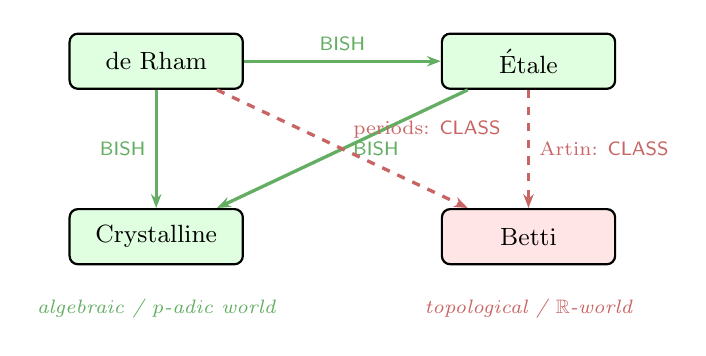
\begin{tikzpicture}[
  cbox/.style={draw, rounded corners=3pt, thick,
    minimum width=2.2cm, minimum height=0.7cm,
    align=center, font=\small},
  node distance=0.8cm
]
  \node[cbox, fill=green!12] (dR) {de Rham};
  \node[cbox, fill=green!12, right=2.5cm of dR] (et) {\'Etale};
  \node[cbox, fill=green!12, below=1.5cm of dR] (crys) {Crystalline};
  \node[cbox, fill=red!10, right=2.5cm of crys] (betti) {Betti};

  % BISH comparisons
  \draw[arr, bishgreen!70, very thick] (dR) -- (et)
    node[midway, above, font=\scriptsize] {\BISH};
  \draw[arr, bishgreen!70, very thick] (dR) -- (crys)
    node[midway, left, font=\scriptsize] {\BISH};
  \draw[arr, bishgreen!70, very thick] (et) -- (crys)
    node[midway, right, font=\scriptsize] {\BISH};

  % CLASS comparisons
  \draw[arr, classred!70, very thick, dashed] (dR) -- (betti)
    node[midway, above right, font=\scriptsize] {periods: \CLASS};
  \draw[arr, classred!70, very thick, dashed] (et) -- (betti)
    node[midway, right, font=\scriptsize] {Artin: \CLASS};

  % Labels
  \node[below=0.3cm of crys, font=\scriptsize\itshape, bishgreen!70] {algebraic / $p$-adic world};
  \node[below=0.3cm of betti, font=\scriptsize\itshape, classred!70] {topological / $\mathbb{R}$-world};
\end{tikzpicture}
\caption{Comparison isomorphisms and their costs. Within the algebraic/$p$-adic world (green): all comparisons are \BISH. Any comparison that crosses into the topological/$\mathbb{R}$-world (red) costs \CLASS. This is the Archimedean obstruction in one picture.}
\label{fig:comparison-costs}
\end{figure}

\subsection*{The Hodge Decomposition: Sorting Holes by Type}

We said cohomology counts ``holes'' of various dimensions. But not all holes are alike. Some arise from algebraic equations (polynomial subvarieties), while others are purely topological (they exist only because the space has a complicated shape when viewed over $\mathbb{C}$). The \textbf{Hodge decomposition} sorts holes by their algebraic character.

\textbf{A crucial step: from $\mathbb{Q}$ to $\mathbb{C}$.} Until now, we have been studying varieties over $\mathbb{Q}$---looking for rational solutions. To access the Hodge decomposition, we must pass from rational solutions to \emph{complex} solutions, studying the shape $X(\mathbb{C})$ as a complex manifold. This is the point where the Archimedean place enters: $\mathbb{C}$ is built from $\mathbb{R}$ (as $\mathbb{R}[i]$), and anything that depends on the topology of $\mathbb{C}$ inherits the logical cost of $\mathbb{R}$.

Over $\mathbb{C}$, each cohomology group $H^k$ breaks into finer pieces labeled by two numbers $(p, q)$ with $p + q = k$:
\[
  H^k(X) \;=\; \bigoplus_{p+q=k} H^{p,q}(X).
\]
What do $p$ and $q$ measure? Think of $p$ as counting the ``algebraic directions'' (technically, holomorphic differentials $dz$) and $q$ as counting the ``conjugate directions'' (anti-holomorphic differentials $d\bar{z}$). A class in $H^{2,0}$ is ``purely algebraic'' (two holomorphic directions, no conjugate). A class in $H^{0,2}$ is ``purely conjugate.'' The interesting classes are those in $H^{p,p}$---\emph{balanced equally between algebraic and conjugate directions}. These are the potential candidates for coming from actual polynomial subvarieties.

\begin{analogybox}[Analogy: frequencies in a sound]
A musical note can be decomposed into frequencies (Fourier analysis). Each frequency captures a different ``mode of vibration.'' The $(p,q)$ decomposition does the same for cohomological holes: it sorts each hole by how it vibrates in the holomorphic direction ($p$) versus the anti-holomorphic direction ($q$).

A class of type $(p,p)$ is like a ``pure tone at the fundamental frequency''---balanced, symmetric, the most algebraic kind of hole. The Hodge conjecture asks: can every pure tone be produced by an instrument (an algebraic subvariety)?
\end{analogybox}

A \textbf{Hodge class} is a cohomology class of type $(p,p)$ that is also rational (lives over $\mathbb{Q}$, not just $\mathbb{C}$). The \textbf{Hodge conjecture} (a Clay Millennium Problem, worth \$1M) says: every Hodge class is algebraic---it genuinely comes from a polynomial subvariety.

\medskip
\textbf{Why does this cost \CLASS?} The question is: given a cohomology class $\alpha \in H^{2p}(X, \mathbb{Q})$, does it land in the $(p,p)$ piece of the Hodge decomposition? To answer this, you need the Hodge decomposition \emph{itself}---and computing it requires hard analysis over $\mathbb{R}$.

Here is the chain of reasoning:
\begin{enumerate}
  \item \textbf{The Hodge theorem} says: every cohomology class has a unique ``harmonic representative''---a differential form $\omega$ satisfying the Laplace equation $\Delta \omega = 0$. This harmonic representative has a definite type $(p,q)$.
  \item \textbf{But solving $\Delta \omega = 0$} is a partial differential equation (PDE) on the complex manifold $X(\mathbb{C})$. Under the hood, this involves elliptic PDE theory: integration over $\mathbb{R}$, convergence of infinite series, existence of solutions via compactness arguments. All of this requires the completeness and order properties of $\mathbb{R}$---the Archimedean place.
  \item \textbf{The cost structure therefore bifurcates:}
  \begin{itemize}
    \item \emph{Detection} (``Is $\alpha$ of type $(p,p)$?'') requires solving the PDE, which requires $\mathbb{R}$: \textbf{\CLASS}.
    \item \emph{Verification} (``Given that $Z$ is an algebraic subvariety, does its fundamental class land in $H^{p,p}$?'') is pure algebra: compute the cycle class map $[Z] \mapsto H^{2p}$, which is a finite polynomial operation: \textbf{\BISH}.
  \end{itemize}
\end{enumerate}

This detection/verification split is the Archimedean obstruction in its purest form. You can \emph{check} algebraicity cheaply; you cannot \emph{find} it cheaply. The CRM program identified this as a universal pattern: across all five great conjectures, detection (``does this object have property $P$?'') costs \CLASS, while verification (``is this known candidate correct?'') costs \BISH.

\subsection*{Algebraic Cycles: Subshapes Inside Shapes}

An \textbf{algebraic cycle} on $X$ is a formal sum of subvarieties---a ``grocery list with quantities'': $Z = 3 \cdot C_1 - 2 \cdot C_2 + C_3$, where each $C_i$ is itself a variety sitting inside $X$, and the integer coefficients are multiplicities (negative signs indicate orientation reversal). The \textbf{codimension} is how much smaller the subvariety is: a curve inside a surface has codimension~1; a point inside a surface has codimension~2.

Two cycles can be ``the same'' even when they look different geometrically. For example, on a surface, two curves that can be continuously deformed into each other represent the same cohomology class, even though they are defined by different polynomial equations. But there are different notions of ``same,'' and which one you use has dramatic consequences for logical cost:
\begin{itemize}
  \item \textbf{Homological equivalence:} two cycles are the same if they represent the same class in cohomology. Testing this requires computing cohomology---potentially \CLASS, since Betti cohomology involves integration over $\mathbb{R}$.
  \item \textbf{Numerical equivalence:} two cycles are the same if they have the same \emph{intersection numbers} with every other cycle. The \textbf{intersection number} of two curves on a surface counts how many times they cross (with signs for orientation and multiplicities for tangencies). This is a finite integer, computable by polynomial algebra: \BISH.
\end{itemize}

\textbf{Standard Conjecture D} says these two notions agree. If true, this would be a spectacular constructivization: you could test whether two cycles are cohomologically equivalent by computing finitely many intersection numbers---finite arithmetic instead of infinite topological computation. In CRM language, Standard Conjecture~D would allow you to replace a \CLASS{} test with a \BISH{} test.

\subsection*{Elliptic Curves, Abelian Varieties, and Jacobians}

An \textbf{elliptic curve} is a smooth cubic curve with a marked point. Example: $y^2 + y = x^3 - x$ with the point $(0,0)$. The key miracle: the rational points on an elliptic curve form a \emph{group}---you can ``add'' two points using a beautiful geometric construction:

\begin{analogybox}[The chord-and-tangent law]
To add two points $P$ and $Q$ on an elliptic curve: draw the straight line through $P$ and $Q$. Because the curve is a cubic, this line hits the curve in exactly one more point, call it $R$. Now reflect $R$ across the $x$-axis to get $P + Q$. That's it---the group operation is defined by drawing lines and reflecting. When $P = Q$, draw the tangent line instead. This works over any field, and the arithmetic involves only rational operations on coordinates: \BISH.
\end{analogybox}

The \textbf{rank} is the number of independent generators of this group (modulo the finite torsion subgroup). Finding the rank is the central problem of BSD.

An \textbf{abelian variety} is the higher-dimensional generalization: a smooth projective variety that is simultaneously a group (meaning you can ``add'' points, generalizing the chord-and-tangent law). An \textbf{abelian surface} is 2-dimensional; an \textbf{abelian fourfold} is 4-dimensional. Some abelian varieties decompose as products of elliptic curves, but most do not---they are genuinely higher-dimensional objects.

The \textbf{Jacobian} $J(C)$ of a curve $C$ of genus $g$ is a $g$-dimensional abelian variety that packages the curve's essential geometric data (specifically, the divisor class group) into a higher-dimensional group variety. For an elliptic curve (genus~1), the Jacobian is the curve itself. For a genus-4 hyperelliptic curve (the test family in the Hodge campaign), the Jacobian is a 4-dimensional abelian variety.

\begin{figure}[htbp]
\centering
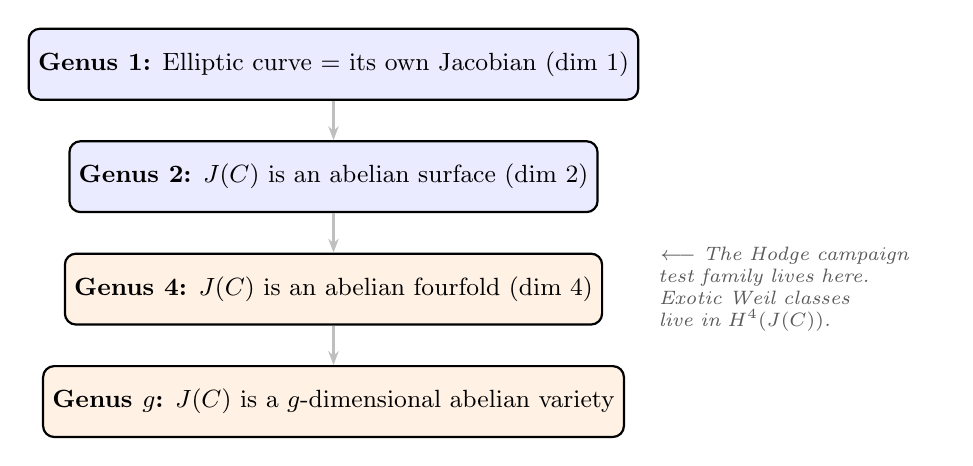
\begin{tikzpicture}[
  gbox/.style={draw, rounded corners=4pt, thick,
    minimum width=5cm, minimum height=0.9cm,
    align=center, font=\small},
  node distance=0.5cm
]
  \node[gbox, fill=blue!8] (g1)
    {\textbf{Genus 1:} Elliptic curve $=$ its own Jacobian (dim 1)};
  \node[gbox, fill=blue!8, below=of g1] (g2)
    {\textbf{Genus 2:} $J(C)$ is an abelian surface (dim 2)};
  \node[gbox, fill=orange!10, below=of g2] (g4)
    {\textbf{Genus 4:} $J(C)$ is an abelian fourfold (dim 4)};
  \node[gbox, fill=orange!10, below=of g4] (gg)
    {\textbf{Genus $g$:} $J(C)$ is a $g$-dimensional abelian variety};
  \draw[arr, gray!50] (g1) -- (g2);
  \draw[arr, gray!50] (g2) -- (g4);
  \draw[arr, gray!50] (g4) -- (gg);
  \node[right=0.6cm of g4, font=\scriptsize, text width=3.5cm, align=left, text=gray!70!black]
    {$\longleftarrow$ \emph{The Hodge campaign\\test family lives here.\\Exotic Weil classes\\live in $H^4(J(C))$.}};
\end{tikzpicture}
\caption{The genus--Jacobian correspondence. Each curve $C$ of genus $g$ produces a $g$-dimensional abelian variety $J(C)$.}
\label{fig:genus-jacobian}
\end{figure}

\subsection*{Heights: Measuring the ``Size'' of a Rational Point}

A \textbf{height function} $h(P)$ assigns a non-negative real number to each rational point, measuring its ``arithmetic complexity.'' For a rational number $a/b$ in lowest terms, the na\"ive height is $\max(|a|, |b|)$. The point $(3/5, 4/5)$ has height 5. The point $(123456/789, 0)$ has height 123456.

The \textbf{N\'eron-Tate canonical height} $\hat{h}$ is a refined version for elliptic curves that is a \emph{quadratic form}: $\hat{h}(P + Q) + \hat{h}(P - Q) = 2\hat{h}(P) + 2\hat{h}(Q)$. It is \textbf{positive-definite}: $\hat{h}(P) = 0$ if and only if $P$ is torsion (finite-order in the group law). This converts the rational-point search from an unbounded problem (search all of $\mathbb{Q}^2$) into a bounded one (search below a height bound).

The \textbf{Northcott property}: for any bound $B$, there are only \emph{finitely many} rational points with $h(P) \leq B$. Combined with positive-definiteness, this makes the search finite---\BISH.

\subsection*{Galois Representations: Symmetry Actions on Cohomology}

The absolute Galois group $\mathrm{Gal}(\overline{\mathbb{Q}}/\mathbb{Q})$ is the group of all ``symmetries'' of the algebraic numbers---all the ways you can permute roots of polynomials with rational coefficients while respecting every polynomial relation among them. For instance, one symmetry sends $\sqrt{2}$ to $-\sqrt{2}$ (both are roots of $x^2 - 2$); another sends $i$ to $-i$ (both roots of $x^2 + 1$). This group is enormous, infinite, and deeply mysterious. No one can write down all its elements.

But we can study it \emph{indirectly}, by watching how it acts on simpler objects. A \textbf{Galois representation} assigns to each symmetry a \emph{matrix}---a concrete, computable object acting on a finite-dimensional vector space built from the geometry of a variety (its cohomology).

\begin{analogybox}[Analogy: studying a shadow]
You cannot see a 4-dimensional object directly. But you can project it onto a 2-dimensional screen and study its shadow. Different projections give different shadows---but together they tell you about the original object. A Galois representation is a ``shadow'' of the Galois group: a finite-dimensional matrix representation that captures part of the group's structure.
\end{analogybox}

Where do these vector spaces come from? From \'etale cohomology. For a variety $X$ over $\mathbb{Q}$ and a prime $\ell$, the \'etale cohomology $H^k_{\text{\'et}}(X, \mathbb{Q}_\ell)$ is a vector space over the $\ell$-adic numbers that carries a natural action of the Galois group:
\[
  \rho\colon \mathrm{Gal}(\overline{\mathbb{Q}}/\mathbb{Q}) \;\longrightarrow\; \mathrm{GL}_n(\mathbb{Q}_\ell).
\]

\textbf{Concrete example.} Consider the elliptic curve $E\colon y^2 + y = x^3 - x$ (this is the curve ``37a1'' from Paper~95). For each prime $p \neq 37$, the trace of the Galois action on the Tate module of $E$ is:
\[
  a_p \;=\; p + 1 - \#E(\mathbb{F}_p),
\]
where $\#E(\mathbb{F}_p)$ means: reduce the equation modulo $p$ and count solutions. For example: modulo~2 the curve $y^2 + y = x^3 - x$ has 5~solutions, so $a_2 = 2 + 1 - 5 = -2$. Similarly $a_3 = -3$, $a_5 = -2$, $a_7 = -2$, and so on. These are just point counts over finite fields---pure finite arithmetic, no integration, no topology. \BISH.

This is the key insight: Galois representations live in the \'etale realization, which is non-Archimedean. Linear algebra over $\mathbb{Q}_\ell$ is \BISH{} (because $\mathbb{Q}_\ell$ is a completion at a finite prime, so its arithmetic involves no Archimedean comparisons). Much of modern number theory consists of studying Galois representations and their internal structure (semisimplicity, irreducibility, determinant, ramification)---all of which is algebraic and constructive. The logical cost enters only when you try to \emph{match} a Galois representation with an analytic object (a modular form, an $L$-function)---because that matching crosses the comparison-isomorphism boundary into the Archimedean world.

\subsection*{Modular Forms: Functions with Extreme Symmetry}

Start with a simple observation: the sine function satisfies $\sin(x + 2\pi) = \sin(x)$. It has one symmetry (translation by $2\pi$). A modular form is a function with \emph{infinitely many} symmetries---not just translations, but also inversions, rotations, and combinations thereof. These symmetries are so constraining that the function is almost entirely determined by them.

\begin{analogybox}[Analogy: a kaleidoscope]
A kaleidoscope takes a small pattern and replicates it using mirrors into a highly symmetric image. A modular form is the mathematical analogue: a small amount of data (the Fourier coefficients $a_n$) is replicated by a large symmetry group into a rigid global function. The symmetry is so extreme that knowing the first few $a_n$ determines \emph{all} of them. This is why modular forms are computable: infinite symmetry makes finite data sufficient.
\end{analogybox}

Formally, a \textbf{modular form} of weight $k$ and level $N$ is a holomorphic function $f(\tau)$ on the upper half-plane $\mathfrak{H} = \{\tau \in \mathbb{C} : \mathrm{Im}(\tau) > 0\}$ satisfying:
\[
  f\!\left(\frac{a\tau + b}{c\tau + d}\right) = (c\tau + d)^k f(\tau)
  \quad \text{for all } \begin{pmatrix} a & b \\ c & d \end{pmatrix} \in \Gamma_0(N).
\]
Here $\Gamma_0(N)$ is the group of $2 \times 2$ integer matrices with determinant~1 whose lower-left entry is divisible by $N$. Do not be intimidated by this formula. It says: if you apply any of these matrix transformations to $\tau$ (a M\"obius transformation $\tau \mapsto (a\tau+b)/(c\tau+d)$), the function $f$ transforms in a predictable way controlled by the weight~$k$. The space of such functions is finite-dimensional (the dimension is given by a formula involving $k$, $N$, and the genus of the modular curve), so \emph{every} modular form is a finite linear combination of basis elements. Moreover, the \textbf{Sturm bound} ($\approx kN/12$) tells you that a modular form is completely determined by finitely many of its Fourier coefficients. This is why they are computable.

Every modular form has a \textbf{Fourier expansion} $f(\tau) = \sum_{n \geq 0} a_n q^n$ where $q = e^{2\pi i \tau}$. The coefficients $a_n$ encode arithmetic information. For an elliptic curve $E$ over $\mathbb{Q}$:
\[
  a_p = p + 1 - \#E(\mathbb{F}_p) \quad\text{(the ``error term'' in the point count over $\mathbb{F}_p$).}
\]
Computing $a_p$ is pure finite arithmetic: count solutions modulo $p$, subtract. \BISH.

The \textbf{modularity theorem} (Wiles, Taylor-Wiles, Breuil-Conrad-Diamond-Taylor) is the bridge between algebra and analysis. More precisely: for every elliptic curve $E$ over $\mathbb{Q}$, there exists a weight-2 modular form $f$ whose Fourier coefficients $a_n(f)$ equal the point-count data $a_n(E)$ for all~$n$. The sequences are identical---the same integers appear on both sides---but one sequence comes from counting points on a curve (algebra, \BISH) and the other from a symmetric function on the complex upper half-plane (analysis, \CLASS).

In CRM language: the modularity theorem is a \emph{comparison isomorphism} between the \'etale realization (Galois representation of $E$: \BISH) and the automorphic realization (modular form on $\mathfrak{H}$: \CLASS). The data on both sides is algebraic; the \emph{proof} that they match crosses the Archimedean place---it must invoke properties of complex analysis (analytic continuation, $L$-functions, convergence) that require the completeness of $\mathbb{R}$.

\subsection*{Motives: The Universal Blueprint}

We have seen that a single variety can be studied through multiple cohomology theories (Betti, de Rham, \'etale, crystalline), all giving the same dimensions. A \textbf{motive} is Grothendieck's conjectural answer to the question: \emph{what is the common object behind all these cohomology theories?} Just as a single integer can be viewed in different bases (decimal, binary, hexadecimal) without changing the integer itself, a single motive can be ``viewed'' through different cohomology theories without changing the underlying mathematical content.

\begin{analogybox}[Analogy: the DNA analogy]
A variety $X$ is an organism. Its motive is its DNA. Betti cohomology, de Rham cohomology, \'etale cohomology, and crystalline cohomology are different medical tests (blood test, MRI, genetic screen, biopsy) that each reveal partial information. The motive is the complete genome: every test is recoverable from it. The genome itself is purely informational (\BISH). The individual tests may require lab equipment (\CLASS{} for Betti, \BISH{} for \'etale). The cost depends on which test you run, not on the genome.
\end{analogybox}

A \textbf{realization functor} extracts one type of cohomology from the motive. The CRM cost of the realization depends on whether it ``passes through $\mathbb{R}$''---meaning whether the extraction process requires completing $\mathbb{Q}$ at the Archimedean place (working over $\mathbb{R}$ or $\mathbb{C}$) or stays within the algebraic/$p$-adic world (see Figure~\ref{fig:cohomology-flavours}).

Why is the motive itself \BISH? Because motives (in the conjectural formulation) are defined by \emph{algebraic correspondences}: polynomial maps between varieties, composed and identified by finite algebraic operations. No real analysis, no integration, no topology. The motive is pure algebra.

This is the central insight of Paper~98: \textbf{the motive is always \BISH; the cost lives in the realization.} A theorem about a variety is a statement about its motive. To \emph{prove} the theorem, you must apply one or more realization functors and comparison isomorphisms. The logical cost of the proof is determined by which realizations and comparisons you use---specifically, by whether any of them pass through $\mathbb{R}$. If you can find a proof path that stays entirely within the algebraic/$p$-adic world, the theorem is \BISH. If every proof path must cross into the Betti/Hodge/automorphic world, the theorem is irreducibly \CLASS. Most interesting theorems are somewhere in between: a large \BISH{} core with isolated \CLASS{} nodes at the points where comparison isomorphisms force a crossing.

\subsection*{$p$-Adic Numbers: An Alternative to $\mathbb{R}$}

The real numbers $\mathbb{R}$ are the completion of $\mathbb{Q}$ using the usual absolute value: two rationals are ``close'' if their difference is small. The \textbf{$p$-adic numbers} $\mathbb{Q}_p$ are an alternative completion: two rationals are ``close'' if their difference is divisible by a high power of a prime $p$.

Example: in $\mathbb{Q}_5$, the numbers 1 and 126 are ``close'' because $126 - 1 = 125 = 5^3$. But 1 and 2 are ``far apart'' (differ by 1, which is not divisible by 5).

The \textbf{Archimedean place} is the place ``at infinity'' where we complete to $\mathbb{R}$. The \textbf{non-Archimedean places} are the primes $p$ where we complete to $\mathbb{Q}_p$. The CRM program found: $\mathbb{R}$ is the sole source of \CLASS{} content. All $\mathbb{Q}_p$ are \BISH.

\subsection*{Quick Reference Card}

\begin{table}[htbp]
\centering\small
\caption{Jargon decoder for the rest of this monograph.}
\renewcommand{\arraystretch}{1.25}
\begin{tabular}{@{}l p{6cm}@{}}
\toprule
\textbf{Term} & \textbf{Plain English} \\
\midrule
Variety & Shape defined by polynomial equations \\
Smooth, projective & No corners; closed up at infinity \\
Cohomology $H^k(X)$ & Vector spaces counting $k$-dimensional holes \\
Hodge type $(p,p)$ & The ``most algebraic'' kind of hole \\
Algebraic cycle & Formal sum of polynomial subshapes \\
Elliptic curve & Smooth cubic curve with a group law \\
Rank & Number of independent rational points \\
Abelian variety & Higher-dimensional elliptic curve (a projective group) \\
Jacobian $J(C)$ & The abelian variety encoding a curve's geometry \\
Height $h(P)$ & Arithmetic complexity of a rational point \\
Northcott property & Finitely many points below any height bound \\
Galois representation & Symmetry action encoded as matrices \\
Modular form & Function with extreme symmetry on the upper half-plane \\
Hecke eigenvalue $a_p$ & Error term in point count mod $p$ \\
Motive & Universal DNA of a variety (encodes all cohomologies) \\
Realization functor & Extracting one cohomology type from the motive \\
$\mathbb{Q}_p$ ($p$-adic numbers) & Alternative to $\mathbb{R}$; completion at a prime $p$ \\
\bottomrule
\end{tabular}
\label{tab:jargon}
\end{table}


%══════════════════════════════════════════════════════════
% CHAPTER 2
%══════════════════════════════════════════════════════════
\chapter{The Five Conjectures}

\paperref{1--44} established the physics ceiling: \BISH{} + \LPO. Now the program turns to pure mathematics. Does the same source---the real numbers---explain logical difficulty beyond physics?

%── 2.1 ───────────────────────────────────────────────────
\section{Why Arithmetic Geometry?}

Before introducing the five conjectures formally, here is the key idea in plain language.

\begin{analogybox}[What do these conjectures have in common?]
Each conjecture says: \emph{if something looks geometric from the analytic side, it actually is geometric.} Think of it as a ``no mirages'' principle. When you observe a pattern through one lens (analysis, $L$-functions, cohomology), the conjecture promises there's a concrete geometric object (a curve, a cycle, a rational point) causing that pattern. These conjectures are hard because moving from ``it looks real'' to ``here's the actual object'' requires crossing from analysis (which uses $\mathbb{R}$) to algebra (which doesn't)---and that crossing is where all the logical cost lives.
\end{analogybox}

Five conjectures were chosen for calibration, each connecting algebraic geometry to analysis, each open for decades, each central to modern number theory:

\begin{enumerate}
  \item \textbf{Hodge Conjecture} (1950)---Clay Millennium Problem.
    \emph{Plain English:} If a ``shadow'' in the cohomology of a geometric shape looks like it came from a subshape, it really did come from a subshape.
  \item \textbf{Tate Conjecture} (1965).
    \emph{Plain English:} If a cohomology class is fixed by every symmetry of the number system (Galois group), it must be algebraic.
  \item \textbf{Birch and Swinnerton-Dyer Conjecture} (1965)---Clay Millennium Problem.
    \emph{Plain English:} The number of independent rational solutions to a cubic equation equals the number of times a certain analytic function touches zero at a special point.
  \item \textbf{Fontaine-Mazur Conjecture} (1992).
    \emph{Plain English:} If a $p$-adic symmetry pattern ``looks geometric'' (satisfies certain smoothness conditions), it actually comes from the geometry of an algebraic variety.
  \item \textbf{Weight-Monodromy Conjecture} (1970).
    \emph{Plain English:} When a family of varieties degenerates (develops singularities), the degeneration pattern of the cohomology is controlled by algebraic data---the ``weight'' of the Hodge structure.
\end{enumerate}

Each conjecture asserts that something ``looks right'' from the analytic side (cohomology, $L$-functions, Galois representations) if and only if something ``is right'' on the algebraic side (algebraic cycles, rational points, geometric origin). CRM calibrates the logical cost of moving between these two sides (\paperref{45--49}).


%── 2.2 ───────────────────────────────────────────────────
\section{The Five Conjectures Calibrated}

\begin{figure}[htbp]
\centering
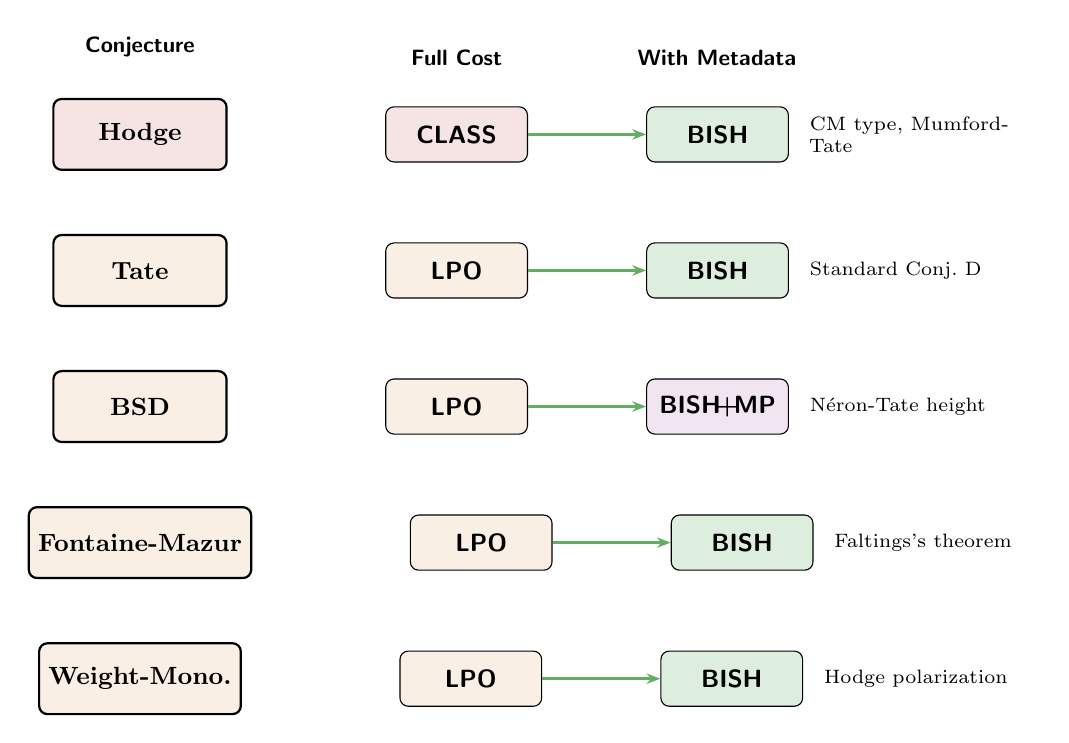
\begin{tikzpicture}[
  conjbox/.style={draw, rounded corners=3pt, thick,
    minimum width=2.2cm, minimum height=0.9cm,
    align=center, font=\small\bfseries},
  node distance=0.8cm and 1.5cm
]
  % Left column: conjecture names
  \node[conjbox, fill=classred!12] (hodge) {Hodge};
  \node[conjbox, fill=lpoamber!12, below=of hodge] (tate) {Tate};
  \node[conjbox, fill=lpoamber!12, below=of tate] (bsd) {BSD};
  \node[conjbox, fill=lpoamber!12, below=of bsd] (fm) {Fontaine-Mazur};
  \node[conjbox, fill=lpoamber!12, below=of fm] (wm) {Weight-Mono.};

  % Middle column: full cost
  \node[right=2cm of hodge, font=\small\bfseries, fill=classred!12,
        draw, rounded corners=3pt, minimum width=1.8cm,
        minimum height=0.7cm] (hc) {\CLASS};
  \node[right=2cm of tate, font=\small\bfseries, fill=lpoamber!12,
        draw, rounded corners=3pt, minimum width=1.8cm,
        minimum height=0.7cm] (tc) {\LPO};
  \node[right=2cm of bsd, font=\small\bfseries, fill=lpoamber!12,
        draw, rounded corners=3pt, minimum width=1.8cm,
        minimum height=0.7cm] (bc) {\LPO};
  \node[right=2cm of fm, font=\small\bfseries, fill=lpoamber!12,
        draw, rounded corners=3pt, minimum width=1.8cm,
        minimum height=0.7cm] (fc) {\LPO};
  \node[right=2cm of wm, font=\small\bfseries, fill=lpoamber!12,
        draw, rounded corners=3pt, minimum width=1.8cm,
        minimum height=0.7cm] (wc) {\LPO};

  % Right column: with metadata
  \node[right=1.5cm of hc, font=\small\bfseries, fill=bishgreen!15,
        draw, rounded corners=3pt, minimum width=1.8cm,
        minimum height=0.7cm] (hm) {\BISH};
  \node[right=1.5cm of tc, font=\small\bfseries, fill=bishgreen!15,
        draw, rounded corners=3pt, minimum width=1.8cm,
        minimum height=0.7cm] (tm) {\BISH};
  \node[right=1.5cm of bc, font=\small\bfseries, fill=mppurple!10,
        draw, rounded corners=3pt, minimum width=1.8cm,
        minimum height=0.7cm] (bm) {\BISH{}\!+\!\MP};
  \node[right=1.5cm of fc, font=\small\bfseries, fill=bishgreen!15,
        draw, rounded corners=3pt, minimum width=1.8cm,
        minimum height=0.7cm] (fmm) {\BISH};
  \node[right=1.5cm of wc, font=\small\bfseries, fill=bishgreen!15,
        draw, rounded corners=3pt, minimum width=1.8cm,
        minimum height=0.7cm] (wmm) {\BISH};

  % Arrows
  \foreach \s/\t in {hc/hm, tc/tm, bc/bm, fc/fmm, wc/wmm} {
    \draw[arr, bishgreen!70, very thick] (\s) -- (\t);
  }

  % Headers
  \node[above=0.4cm of hodge, font=\footnotesize\bfseries\sffamily] {Conjecture};
  \node[above=0.4cm of hc, font=\footnotesize\bfseries\sffamily] {Full Cost};
  \node[above=0.4cm of hm, font=\footnotesize\bfseries\sffamily, text width=2cm, align=center]
    {With Metadata};

  % Metadata labels (right side)
  \node[right=4pt of hm, font=\scriptsize, text width=2.5cm] {CM type, Mumford-Tate};
  \node[right=4pt of tm, font=\scriptsize, text width=2.5cm] {Standard Conj.\ D};
  \node[right=4pt of bm, font=\scriptsize, text width=2.5cm] {N\'eron-Tate height};
  \node[right=4pt of fmm, font=\scriptsize, text width=2.5cm] {Faltings's theorem};
  \node[right=4pt of wmm, font=\scriptsize, text width=2.5cm] {Hodge polarization};
\end{tikzpicture}
\caption{Every conjecture drops from \LPO/\CLASS{} to \BISH{} (or \BISH{} + \MP) when provided the right algebraic metadata. The green arrows show de-omniscientizing descent: algebraic data substitutes for the oracle.}
\label{fig:five-conjectures}
\end{figure}

Each conjecture exhibits the same phenomenon. The full statement costs \LPO{} or \CLASS{}---you need an oracle to verify it in general---but providing the right algebraic data substitutes for the oracle and drops the cost to \BISH.

\smallskip
\noindent\textbf{Notation.} When we write $\LPO(\mathbb{R})$ or $\LPO(\mathbb{Q}_\ell)$, we mean that the omniscience principle is applied to sequences valued in $\mathbb{R}$ or $\mathbb{Q}_\ell$ respectively. The subscript identifies \emph{which number system} requires the oracle. This matters because some oracles are more expensive than others: $\LPO(\mathbb{R})$ involves the full Archimedean continuum, while $\LPO(\mathbb{Q}_\ell)$ involves $\ell$-adic completions. Both are instances of the same logical pattern---deciding whether a sequence has a nonzero term---but applied to different ground fields.
\smallskip

\begin{itemize}
  \item \textbf{Hodge (\paperref{49}):} Full cost \CLASS. With CM type or Mumford-Tate group metadata, the Hodge test becomes finite $\mathbb{Q}$-linear algebra: \BISH.
  \item \textbf{Tate (\paperref{46}):} Full cost $\LPO(\mathbb{Q}_\ell)$. Standard Conjecture~D (numerical $=$ homological equivalence) makes cycle comparison finite arithmetic: \BISH.
  \item \textbf{BSD (\paperref{48}):} Full cost $\LPO(\mathbb{R})$. The N\'eron-Tate height (positive-definite on $\mathbb{R}$) bounds the rational-point search, converting it from unbounded to bounded: \BISH{} + \MP. The residual \MP{} is subtle: the height gives you \emph{finiteness}---only finitely many rational points of bounded height---but not an explicit \emph{enumeration bound} on how long the search takes. You know the search terminates (Markov's Principle), but you cannot compute in advance exactly when it will stop.
  \item \textbf{Fontaine-Mazur (\paperref{47}):} Full cost $\LPO(\mathbb{Q}_p)$. Faltings's theorem (geometric origin of $p$-adic representations) makes the comparison algebraic: \BISH.
  \item \textbf{Weight-Monodromy (\paperref{45}):} Full cost \LPO. Hodge polarization (geometric origin) reduces the monodromy test to combinatorics: \BISH.
\end{itemize}

The metadata is always a \textbf{positive-definite structure} that exploits $u(\mathbb{R}) = \infty$: an inner product, a height, a polarization. The oracle (``search over infinity'') is replaced by a computation (``search within a finite ball defined by the positive-definite form''). This is the core mechanism.


%── 2.3 ───────────────────────────────────────────────────
\section{De-Omniscientizing Descent}

The shared pattern across all five conjectures has a name: \textbf{de-omniscientizing descent}. Before the formal version, here is a concrete example.

\begin{analogybox}[Concrete Example: Finding a Book in a Library]
\textbf{Without metadata (LPO):} You walk into an infinite library and are told ``a book about topology is in here somewhere.'' To find it, you must check every shelf, potentially forever. This is an oracle-level search.

\textbf{With metadata (BISH):} The librarian says ``the topology section is in aisle 7, shelves 3--5.'' Now you walk to a specific, bounded location and check three shelves. Same book, same library, but the metadata (the catalogue system) converted an infinite search into a finite one.

De-omniscientizing descent = installing the catalogue system. The five conjectures each have their own version of ``the catalogue'': a positive-definite structure (height function, CM type, polarization) that bounds the search.
\end{analogybox}

The pattern works like this:

\begin{enumerate}
  \item A theorem, stated in full generality, requires an oracle (\LPO{} or \CLASS) to verify.
  \item The theorem has a natural ``algebraic companion''---a structural condition (like Standard Conjecture~D, or geometric origin of eigenvalues, or positive-definite height) that, if true, provides the same information the oracle would.
  \item When the algebraic companion is available, the cost drops to \BISH. The oracle is replaced by a computation.
\end{enumerate}

The algebraic companion always involves the real numbers, specifically the Archimedean place. It exploits the fact that $\mathbb{R}$ admits positive-definite forms ($u(\mathbb{R}) = \infty$) to convert an unbounded oracle query into a bounded algebraic computation.

\begin{figure}[htbp]
\centering
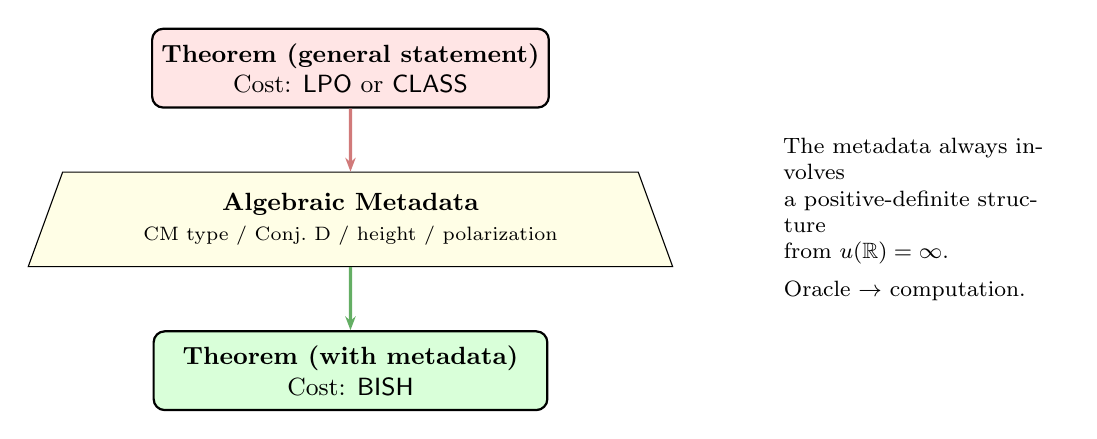
\begin{tikzpicture}[
  node distance=1cm
]
  % Top: generic theorem
  \node[draw, rounded corners=4pt, thick, fill=red!10,
        minimum width=5cm, minimum height=1cm,
        align=center, font=\small] (top)
    {\textbf{Theorem (general statement)}\\
     Cost: \LPO{} or \CLASS};

  % Funnel
  \node[draw, trapezium, trapezium angle=70, fill=yellow!10,
        minimum width=3cm, minimum height=1.2cm,
        align=center, font=\small, below=0.8cm of top] (funnel)
    {\textbf{Algebraic Metadata}\\
     {\scriptsize CM type / Conj.~D / height / polarization}};

  % Bottom: reduced cost
  \node[draw, rounded corners=4pt, thick, fill=green!15,
        minimum width=5cm, minimum height=1cm,
        align=center, font=\small, below=0.8cm of funnel] (bottom)
    {\textbf{Theorem (with metadata)}\\
     Cost: \BISH};

  \draw[arr, very thick, classred!60] (top) -- (funnel);
  \draw[arr, very thick, bishgreen!70] (funnel) -- (bottom);

  % Side annotation
  \node[right=1.5cm of funnel, font=\footnotesize, text width=3.5cm, align=left]
    {The metadata always involves\\a positive-definite structure\\
     from $u(\mathbb{R}) = \infty$.\\[4pt]
     Oracle $\to$ computation.};
\end{tikzpicture}
\caption{De-omniscientizing descent: algebraic metadata replaces the oracle, dropping the cost from \LPO/\CLASS{} to \BISH.}
\label{fig:descent}
\end{figure}

\begin{analogybox}[Analogy: GPS vs.\ Street Signs]
\CLASS{} is like a GPS that magically knows where everything is. \BISH{} is like navigating with a physical map and street signs. The ``algebraic metadata'' is the street signs: if someone installs enough of them (CM type, Mumford-Tate group, algebraic spectrum), you can navigate without the GPS. De-omniscientizing descent is the process of identifying exactly which street signs you need.
\end{analogybox}


%── 2.4 ───────────────────────────────────────────────────
\section{The Three-Invariant Hierarchy}

\paperref{67} (``The Motive Is a Decidability Certificate'') synthesized the calibration data into a classification system. Three numerical invariants determine the logical cost of any motivic cycle-search problem.

\begin{analogybox}[Analogy: Three Dimensions of Search Difficulty]
Imagine searching for a lost object. Three factors determine how hard the search is:
\begin{itemize}
  \item \textbf{Room size} ($=$ rank $r$): How many dimensions is the search space? A line is easier to search than a plane, which is easier than a room.
  \item \textbf{Depth underground} ($=$ Hodge level $\ell$): How many layers deep is the object buried? Surface objects are easy; deep objects require excavation.
  \item \textbf{Minimum object size} ($=$ Lang constant $c$): Is there a minimum size below which objects can't hide? If the smallest possible object is 1 cm, you only need a coarse-enough net to catch everything.
\end{itemize}
Large $r$ makes the search harder (more dimensions). Large $\ell$ makes it harder (deeper burial). Large $c$ makes it \emph{easier} (bigger objects are easier to find).
\end{analogybox}

Formally:
\begin{itemize}
  \item \textbf{Rank $r$}---the dimension of the algebraic cycle space. Higher rank means more candidates to check.
  \item \textbf{Hodge level $\ell$}---how deep in the Hodge filtration the class sits. Higher level means farther from the algebraic surface.
  \item \textbf{Lang constant $c$}---the effective lower bound on height. Lang's height conjecture predicts that for a curve $C$ of genus $g \geq 2$, every rational point $P$ satisfies $\hat{h}(P) \geq c(C) > 0$, where $\hat{h}$ is the N\'eron-Tate canonical height. When $c > 0$, non-trivial cycles can't be arbitrarily small, and the search is bounded.
\end{itemize}

Together, $(r, \ell, c)$ classify the full decidability landscape. \paperref{67} verified this across 53 formalizations totalling 86,898+ lines of Lean~4 code.


%── 2.5 ───────────────────────────────────────────────────
\section{FLT Is \WKL}\label{sec:flt}

The most surprising calibration result.

\begin{analogybox}[The Skyscraper That's One Story Tall]
Fermat's Last Theorem: $x^n + y^n = z^n$ has no integer solutions for $n \geq 3$. Proved by Andrew Wiles in 1995 in a 129-page paper deploying Galois representations, modular forms, deformation rings, and Hecke algebras. This proof is one of the most complex in the history of mathematics.

You would expect it to be logically expensive---surely 129 pages of deep mathematics need powerful axioms? CRM's verdict: \textbf{CRM(FLT) = \WKL.} The sole non-constructive node is the inverse limit in Taylor--Wiles patching---non-Archimedean compactness, not Archimedean analysis.

The 129 pages are almost entirely \emph{scaffolding}---complex but constructive. The theorem sits one floor above ground: the \WKL{} in patching is irreducible (Calibration Theorem~II), but every other component is \BISH.
\end{analogybox}

\paperref{68} audited the Wiles proof stage by stage. Stages 2--4 (deformation theory, Hecke algebra, numerical criterion) are all \BISH. Stage~5 (Taylor--Wiles patching) splits: the prime search is \BISH{} (effective Chebotarev bounds), but the inverse limit assembling $R_\infty$ from finite local rings is \WKL. Stage~1 (Langlands--Tunnell, weight-1 forms) costs \WLPO, but this is an artifact: Kisin's $p=2$ dihedral bypass eliminates it. With Kisin's route, $\mathrm{CRM}(\mathrm{FLT}) = \WKL$.

\begin{figure}[htbp]
\centering
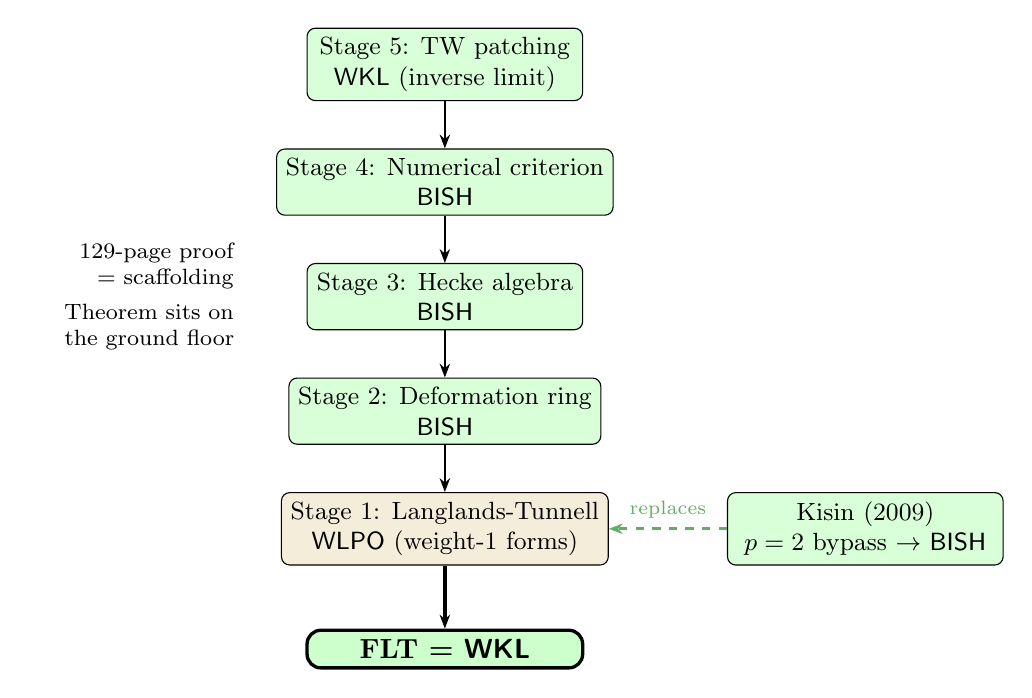
\begin{tikzpicture}[
  sbox/.style={draw, rounded corners=3pt,
    minimum width=3.5cm, minimum height=0.8cm,
    align=center, font=\small},
  node distance=0.6cm
]
  % Stages
  \node[sbox, fill=green!15] (s5) {Stage 5: TW patching\\\WKL{} (inverse limit)};
  \node[sbox, fill=green!15, below=of s5] (s4) {Stage 4: Numerical criterion\\\BISH};
  \node[sbox, fill=green!15, below=of s4] (s3) {Stage 3: Hecke algebra\\\BISH};
  \node[sbox, fill=green!15, below=of s3] (s2) {Stage 2: Deformation ring\\\BISH};
  \node[sbox, fill=wlpogold!15, below=of s2] (s1)
    {Stage 1: Langlands-Tunnell\\\WLPO{} (weight-1 forms)};

  % Kisin bypass
  \node[sbox, fill=green!15, right=1.5cm of s1] (kisin)
    {Kisin (2009)\\$p=2$ bypass $\to$ \BISH};

  \draw[arr] (s5) -- (s4);
  \draw[arr] (s4) -- (s3);
  \draw[arr] (s3) -- (s2);
  \draw[arr] (s2) -- (s1);
  \draw[arr, bishgreen!70, very thick, dashed] (kisin) -- (s1)
    node[midway, above, font=\scriptsize] {replaces};

  % Result
  \node[draw, very thick, rounded corners=5pt, fill=green!20,
        minimum width=3.5cm, below=0.8cm of s1,
        font=\bfseries] (result) {FLT = \WKL};
  \draw[arr, very thick] (s1) -- (result);

  % Annotation
  \node[left=0.8cm of s3, font=\footnotesize, text width=2.5cm, align=right]
    {129-page proof\\= scaffolding\\[3pt]
     Theorem sits on\\the ground floor};
\end{tikzpicture}
\caption{FLT audit (\paperref{68}). Stages 2--4 are \BISH; Stage~5 (TW patching) is \WKL{} (inverse limit); Stage~1 costs \WLPO{} but Kisin's bypass eliminates it. $\mathrm{CRM}(\mathrm{FLT}) = \WKL$: the 129-page proof is mostly scaffolding; the irreducible cost is non-Archimedean compactness.}
\label{fig:flt}
\end{figure}

This is the program's sharpest illustration of a fundamental distinction: \textbf{proof complexity is not logical cost.} Stages 2--4 are intellectually difficult, technically demanding, and involve deep algebra---but they are constructive. Taylor--Wiles patching costs \WKL{} (the inverse limit), but this is non-Archimedean compactness, confirming the Archimedean Principle. Weight-1 modular forms are routine objects---but they cost \WLPO. CRM measures what matters (logical resources), not what impresses (proof difficulty).

\paragraph{The Hecke theta series resolution (\paperref{99}).} Kisin's bypass uses Hecke theta series $\theta_L(\tau) = \sum_{v \in L} q^{Q(v)}$, whose Fourier coefficients are finite lattice sums (\BISH). The \emph{modularity} of $\theta_L$ was originally proved via Poisson summation ($\CLASS$), but \paperref{99} showed three explicit excisions: Poisson $\to$ Mumford algebraic theta, Deligne--Serre $\to$ forward matching, Chebotarev $\to$ effective bounds. The dihedral base case is $\BISH$; the irreducible $\WKL$ is strictly in the patching assembly.


%── 2.6 ───────────────────────────────────────────────────
\section{Function Field Langlands Is \BISH}

If FLT is the surprise, function field Langlands is the explanation.

Over number fields (extensions of $\mathbb{Q}$), the Langlands correspondence connects automorphic forms to Galois representations. This correspondence requires the Archimedean place ($\mathbb{R}$), and its logical cost reflects this: various principles from \WLPO{} to \CLASS{} appear.

Over function fields (extensions of $\mathbb{F}_q(t)$, where $\mathbb{F}_q$ is a finite field), there is no Archimedean place. No $\mathbb{R}$. No $u(\mathbb{R}) = \infty$. And the entire Langlands correspondence is \BISH{} (\paperref{69}). Both proofs---Laurent Lafforgue's for $\mathrm{GL}_n$ and Genestier--V.~Lafforgue's for general reductive groups---are constructive. The boundary between constructive and classical is not ``discrete vs.\ continuous'' but \textbf{algebraic vs.\ transcendental spectral parameters}: over function fields, automorphic representations have algebraic Hecke eigenvalues (elements of $\overline{\mathbb{Q}}$), so every spectral comparison is decidable arithmetic. Over number fields, the Archimedean place introduces transcendental parameters (elements of $\mathbb{C}$ that need not be algebraic), and decidability fails.

This confirms the Archimedean thesis with a clean experiment: remove $\mathbb{R}$, and the cost vanishes.

\begin{keyrefbox}
\textbf{Key references:} \paperref{69} (Function Field Langlands Is \BISH), \paperref{70} (The Archimedean Principle---capstone).
\end{keyrefbox}


%── 2.7 ───────────────────────────────────────────────────
\section{The $h = f$ Identity: A Discovery Through CRM}

\paperref{56--58} report one of the program's most striking discoveries---not a result \emph{about} CRM, but a result \emph{found by} CRM.

\subsection*{Background: exotic Weil classes}

On a \textbf{CM} (complex multiplication) abelian fourfold $X = A \times B$---a product of two abelian surfaces whose endomorphism rings are unusually large (containing a number field, not just $\mathbb{Z}$)---the cohomology contains \textbf{exotic Weil classes}: Hodge classes that are \emph{not} generated by divisor classes. Classical mathematics treats the Hermitian self-intersection number of these classes as an element of $\mathbb{Q}^*/\mathrm{Nm}(K^*)$---the group of nonzero rationals modulo norms from a number field $K$, i.e., an equivalence class rather than a specific number.

\subsection*{What CRM demanded}

The constructive framework refuses equivalence classes. It demands the \emph{exact integer value}. When the program computed this exact value for cyclic Galois totally real cubic fields $F/\mathbb{Q}$, a formula appeared:

\begin{thesisbox}[The $h = f$ Identity (\paperref{56}, Theorem~A)]
For cyclic Galois cubics $F/\mathbb{Q}$ with class-number-one CM field $K$, principal polarizations, and CM signature $(1,2) \times (1,0)$:
\[
  \deg(w_0 \cdot w_0) = \sqrt{\mathrm{disc}(F)} = f
\]
where $w_0$ is the primitive exotic Weil class and $f$ is the arithmetic conductor of $F/\mathbb{Q}$.
\end{thesisbox}

The \textbf{Hermitian self-intersection} $h$ equals the \textbf{arithmetic conductor} $f$. The mechanism: for cyclic cubic extensions, $\mathrm{disc}(F) = f^2$, and the correspondence degree equals $f$.

\subsection*{Extension and correction}

\paperref{57} verified this across all nine class-number-1 imaginary quadratic fields (Baker-Heegner-Stark list): conductors $f = 7, 9, 13, 19, 37, 61, 79, 97, 163$. Eight of nine are prime.

\paperref{58} corrected the formula for fields with class number $h_K > 1$: the exact identity becomes $h \cdot \mathrm{Nm}(\mathfrak{a}) = f$, where $\mathfrak{a}$ is the Steinitz class of the integral Weil lattice. The class group acts as an ``arithmetic compensator'': the topological volume $f^2|\Delta_K|$ is an absolute invariant; the class group redistributes it between the Hermitian metric and the lattice density.

\subsection*{Why CRM found it}

\paperref{58}: ``This result emerged from the constructive framework's insistence on exact integer values rather than equivalence classes modulo norms. The classical literature treats the Hermitian discriminant as an element of $\mathbb{Q}^*/\mathrm{Nm}(K^*)$; the constructive lens demands the exact value, revealing the formula and the role of the class group---structure invisible from the classical perspective.''

The entire computation is \BISH. No omniscience principles are invoked. CRM discovered new mathematics by refusing to round off.


%── 2.8 ───────────────────────────────────────────────────
\section{The Northcott Property: How Metadata Replaces Oracles}

Section~2.3 described de-omniscientizing descent in the abstract. Here is the concrete mechanism that makes it work.

\begin{analogybox}[Analogy: Searching a Field for Buried Treasure]
You're told: ``somewhere in this field, there's buried treasure.'' If the field is infinite, you must dig forever (\LPO---you need an oracle to scan infinitely). But suppose someone gives you a \textbf{metal detector with a range limit}: it can only detect objects within 100 meters of the surface. Now the search region is bounded---the treasure must be in a finite volume of dirt. That's what the \textbf{Northcott property} does: it gives you a ``depth gauge'' (called a \emph{height function}) that guarantees the objects you're looking for all live within a bounded region.

But knowing the region is finite isn't quite enough---you also need to know \emph{how finely to dig}. If you dig with a teaspoon, it could take a billion years. \textbf{Lang's conjecture} provides the second piece: a \emph{minimum spacing guarantee}. The buried objects can't be closer together than some explicit distance $c > 0$. So you know both the volume (Northcott) and the grid spacing (Lang): now you can enumerate everything in bounded time (\BISH).
\end{analogybox}

The \textbf{Northcott property} states: for every bound $B > 0$, the set of rational points on an algebraic variety with \emph{height} $\leq B$ is finite. The \textbf{height} $\hat{h}(P)$ measures the ``arithmetic complexity'' of a point $P$---roughly, how large the numerators and denominators of its coordinates are. Points with small height are simple; points with large height are complicated.

\begin{figure}[htbp]
\centering
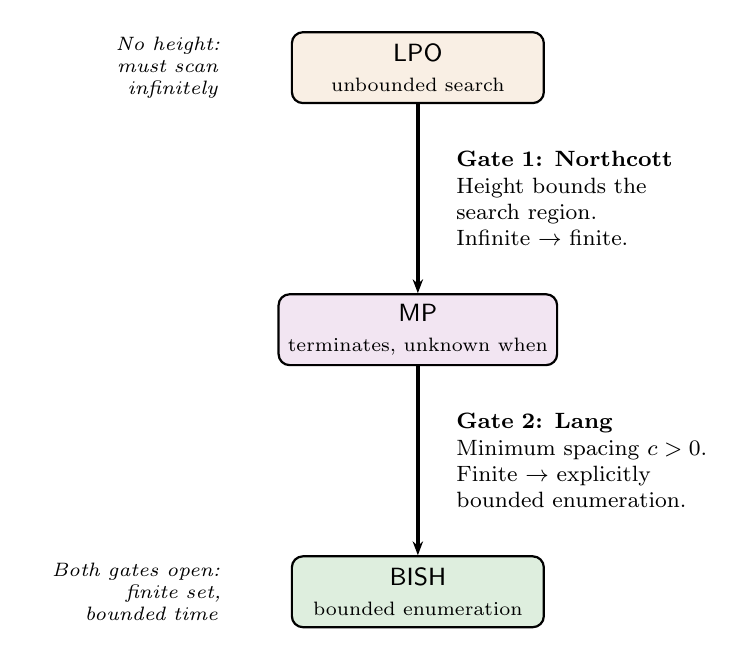
\begin{tikzpicture}[
  gate/.style={draw, rounded corners=4pt, thick,
    minimum width=3.2cm, minimum height=0.9cm,
    align=center, font=\small},
  ann/.style={font=\footnotesize, text width=3.2cm, align=left}
]
  % Three levels — increased vertical spacing to prevent overlap
  \node[gate, fill=lpoamber!12] (lpo)
    {\LPO\\{\scriptsize unbounded search}};
  \node[gate, fill=mppurple!10, below=2.4cm of lpo] (mp)
    {\MP\\{\scriptsize terminates, unknown when}};
  \node[gate, fill=bishgreen!15, below=2.4cm of mp] (bish)
    {\BISH\\{\scriptsize bounded enumeration}};

  % Gates
  \draw[arr, very thick] (lpo) -- (mp)
    node[midway, right=10pt, ann]
      {\textbf{Gate 1: Northcott}\\
       Height bounds the\\
       search region.\\
       Infinite $\to$ finite.};
  \draw[arr, very thick] (mp) -- (bish)
    node[midway, right=10pt, ann]
      {\textbf{Gate 2: Lang}\\
       Minimum spacing $c > 0$.\\
       Finite $\to$ explicitly\\
       bounded enumeration.};

  % Labels
  \node[left=0.8cm of lpo, font=\scriptsize\itshape,
        text width=2.3cm, align=right]
    {No height: must scan\\infinitely};
  \node[left=0.8cm of bish, font=\scriptsize\itshape,
        text width=2.3cm, align=right]
    {Both gates open:\\finite set,\\bounded time};
\end{tikzpicture}
\caption{The Northcott-Lang descent (\paperref{61, 72}). Two gates control the drop from \LPO{} to \BISH. Gate~1 converts infinite search to finite. Gate~2 gives an explicit termination bound. Both exploit the Archimedean place: positive-definite heights exist only over $\mathbb{R}$.}
\label{fig:northcott-lang}
\end{figure}

\textbf{Why this needs $\mathbb{R}$.} The height $\hat{h}$ is a \emph{positive-definite} quadratic form---meaning $\hat{h}(P) = 0$ only for ``trivial'' points (torsion). Positive-definiteness works in every dimension because $u(\mathbb{R}) = \infty$ (recall from \S1.5). Over the $p$-adic numbers, where $u(\mathbb{Q}_p) = 4$, positive-definite forms exist only up to dimension 4---not enough to control the full search space. This is why Northcott is an Archimedean phenomenon.

\textbf{The tight chain (\paperref{72}):} Remove the height $\to$ Northcott fails $\to$ search is unbounded $\to$ you need \LPO. Each implication reverses:
\[
  \text{Positive-definite height} \;\Leftrightarrow\; \text{Northcott} \;\Leftrightarrow\; \BISH\text{ cycle-search}.
\]
This biconditional is proved formally in Lean. It is one of the three DPT axioms (Chapter~3, Axiom~3).


%══════════════════════════════════════════════════════════
% CHAPTER 3
%══════════════════════════════════════════════════════════
\chapter{The DPT Axioms---Three Laws of Logical Cost}

\begin{analogybox}[Chapter Preview: The Three-Legged Stool]
Chapter~2 surveyed five conjectures and found they all drop from expensive to cheap when given the right metadata. This chapter asks: \emph{what is the smallest set of assumptions that makes everything cheap?}

The answer is three axioms---exactly three, no more, no fewer. Think of them as three legs of a stool:
\begin{itemize}
  \item \textbf{Leg 1 (Conjecture D):} ``Can we compare morphisms?'' --- makes it decidable whether two maps between algebraic objects are equal.
  \item \textbf{Leg 2 (Algebraic Spectrum):} ``Can we compare eigenvalues?'' --- makes it decidable whether a number arising from symmetry is zero.
  \item \textbf{Leg 3 (Archimedean Polarization):} ``Can we search for cycles?'' --- converts an infinite search for geometric objects into a finite, bounded one.
\end{itemize}
Each leg is proved to be \emph{irreplaceable}: remove any one, and the stool collapses. No alternative assumption can substitute. This is what ``canonical'' means---not just minimal, but the \emph{only possible} foundation.
\end{analogybox}


%── 3.1 ───────────────────────────────────────────────────
\section{What Problem DPT Solves}

After calibrating five conjectures (Chapter~2), a natural question emerges: is there a minimal set of axioms that, if true, makes the entire motivic cycle-search problem---the central problem of arithmetic geometry---solvable in \BISH?

The answer is yes. The axiom set is called \textbf{DPT (Decidable Polarized Tannakian)}. It consists of three axioms, each governing a distinct domain (morphisms, eigenvalues, cycles). Each axiom is proved to be not just sufficient but \textbf{necessary}---it is the unique condition for constructive decidability in its domain. This makes the axiom set \emph{canonical}, not merely minimal: you cannot substitute a different axiom.

\begin{keyrefbox}
\textbf{Key references:} \paperref{50} (Three Axioms for the Motive), \paperref{72--74} (biconditional proofs).
\end{keyrefbox}


%── 3.2 ───────────────────────────────────────────────────
\section{Axiom 1: Standard Conjecture D---Morphism Decidability}

\begin{analogybox}[Concrete Example First]
You have two roads on a map (two algebraic cycles). Are they ``the same road''? There are two ways to check:

\textbf{Method A (topological):} Walk along both roads and measure whether they pass through the same regions of the map. This requires exploring the entire map---potentially an infinite process.

\textbf{Method B (numerical):} Count how many times each road crosses each landmark (intersection numbers). This is a finite counting exercise.

Conjecture~D says: Methods A and B always give the same answer. If they do, you never need Method~A---you just count intersections. \emph{That's} why Conjecture~D drops the cost from \LPO{} (infinite search) to \BISH{} (finite counting).
\end{analogybox}

\textbf{Formal statement:} Homological equivalence equals numerical equivalence for algebraic cycles. Two ways to measure whether cycles are ``the same''---one using cohomology (a topological invariant), the other using intersection numbers (a numerical invariant)---always agree.

\textbf{CRM role:} Without Conjecture~D, testing whether two morphisms between motives are equal requires \LPO{} (existential search over an infinite cohomological quotient). With Conjecture~D, numerical intersection is a finite computation---\BISH.

\textbf{Biconditional (\paperref{73}):} Standard Conjecture~D is \emph{equivalent} to \BISH{} morphism decidability. Without it, morphism equality costs \LPO, and no alternative axiom can substitute.


%── 3.3 ───────────────────────────────────────────────────
\section{Axiom 2: Algebraic Spectrum---Eigenvalue Decidability}

\begin{analogybox}[Concrete Example First]
A Frobenius operator is like a symmetry that acts on the cohomology of a variety defined over a finite field. Think of it as spinning a crystal and measuring the angles at which it looks the same---these angles are the \textbf{eigenvalues}.

The question: are these eigenvalues ``nice'' numbers (roots of polynomial equations with integer coefficients, like $\sqrt{2}$ or $(1+\sqrt{5})/2$) or ``wild'' numbers (transcendental, like $\pi$ or $e$)?

If they're algebraic (nice): you can compare them exactly using integer arithmetic. ``Is $\sqrt{2} - \sqrt{2} = 0$?'' Yes---provable by squaring.

If they \emph{could} be transcendental (wild): comparing them means testing whether a real number equals zero. That's the equality-test oracle (\WLPO). You can compute more and more decimal digits, but you can never be \emph{certain} a number is exactly zero just from its digits.

Axiom~2 says: the eigenvalues are always algebraic. So comparison is always finite arithmetic, never an infinite decimal check.
\end{analogybox}

\textbf{Formal statement:} Eigenvalues of Frobenius operators have geometric (algebraic) origin---they are roots of polynomials with integer coefficients.

\textbf{CRM role:} Without algebraic spectrum, comparing eigenvalues requires \WLPO{} (testing whether a real number equals zero). With algebraic spectrum, eigenvalue comparison is rational arithmetic---\BISH.

\textbf{Biconditional (\paperref{74}):} Algebraic spectrum is equivalent to \BISH{} eigenvalue decidability.

\textbf{Key subtlety:} The cost of failure here is \WLPO, not \LPO. Eigenvalue comparison is an \emph{equality} test (``is this eigenvalue zero?''), not an existential search (``find a nonzero eigenvalue''). \WLPO{} is strictly weaker than \LPO---equality testing is easier than searching. This intrinsic computational distinction was invisible before CRM.


%── 3.4 ───────────────────────────────────────────────────
\section{Axiom 3: Archimedean Polarization---Cycle Search}

\begin{analogybox}[Concrete Example First]
You're searching for a specific book in a library. Two scenarios:

\textbf{Without Axiom~3:} The library is infinite, and books can be arbitrarily small (even microscopic). You must check every shelf, every corner, every crevice---an unbounded search. This is \LPO.

\textbf{With Axiom~3:} The library is infinite, but every book is at least 1 cm tall (the ``positive-definiteness'' bound). Now you only need to look on shelves---and for any given shelf, only finitely many books fit. The ``height function'' measures how tall a book is. The Northcott property says: for any maximum height, only finitely many books exist below it. The search becomes finite. This is \BISH.

The positive-definiteness bound comes from $\mathbb{R}$ (specifically, from $u(\mathbb{R}) = \infty$---the real numbers support positive-definite forms in every dimension). At $p$-adic places, the bound fails above dimension 4, and the library is unsearchable again.
\end{analogybox}

\textbf{Formal statement:} Cycles of intermediate codimension satisfy an effective positive-definiteness bound.

\textbf{What this means:} When searching for algebraic cycles in middle cohomology (the hardest case), Axiom~3 asserts that positive-definite height functions provide bounded search regions. Without the bound, cycle-search is an infinite scan (\LPO). With the bound, it is a finite computation (\BISH).

\textbf{Biconditional (\paperref{72}):} Archimedean polarization is equivalent to \BISH{} cycle-search decidability. This axiom directly exploits $u(\mathbb{R}) = \infty$: positive-definite quadratic forms exist in every dimension \emph{at the Archimedean place}, and these forms bound the search region.

\textbf{The mechanism is the Northcott property} (Section~2.8). The N\'eron-Tate height $\hat{h}$ is a positive-definite quadratic form on $A(K) \otimes \mathbb{R}$. Positive-definiteness guarantees: for any $B > 0$, the set $\{P : \hat{h}(P) \leq B\}$ is finite. This converts an infinite scan over $A(K)$ into a bounded enumeration---the crucial step from \LPO{} to \BISH. The full descent runs through two gates:

\begin{enumerate}
  \item \textbf{Northcott gate (\LPO{} $\to$ \MP):} Positive-definite height gives finiteness below any bound. The search terminates, but you don't know when.
  \item \textbf{Lang gate (\MP{} $\to$ \BISH):} Lang's conjecture provides an \emph{effective} lower bound $c > 0$ on $\hat{h}(P)$ for non-torsion $P$. Now you know \emph{how large} to search: enumerate all lattice points with $\hat{h}(P) \leq c$. Bounded time. \BISH.
\end{enumerate}

Without the Archimedean place, positive-definite forms in arbitrary dimension do not exist ($u(\mathbb{Q}_p) = 4$), Northcott fails, and cycle-search remains \LPO. This is why Axiom~3 is ``Archimedean.''


%── 3.5 ───────────────────────────────────────────────────
\section{The DPT Triangle}

\begin{figure}[htbp]
\centering
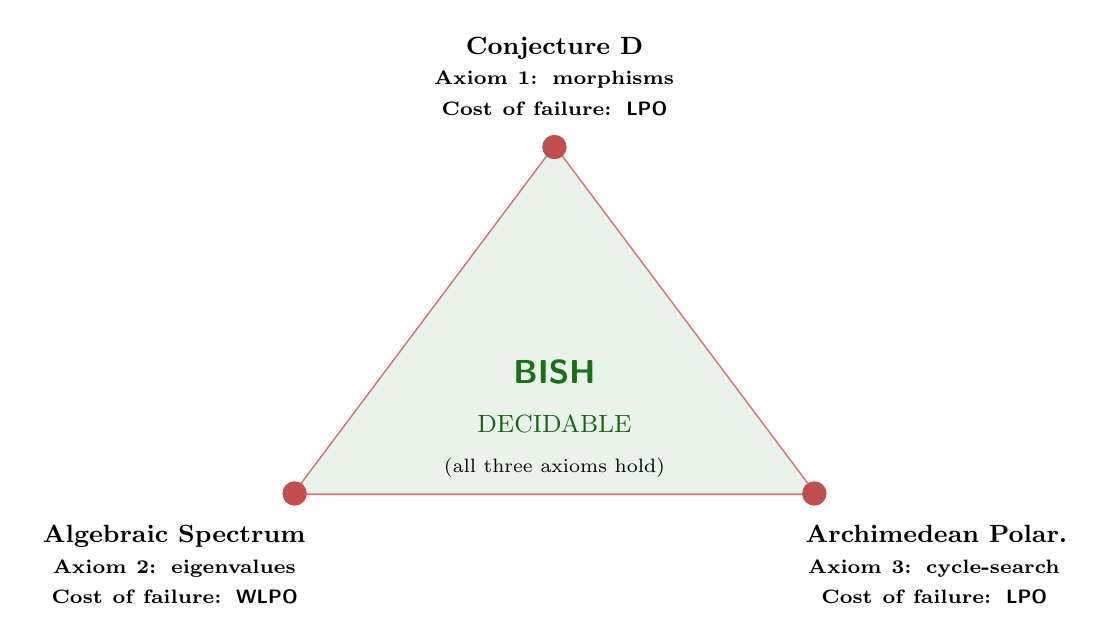
\begin{tikzpicture}[scale=1.1]
  % Triangle
  \coordinate (A) at (0, 4);     % top
  \coordinate (B) at (-3, 0);    % bottom-left
  \coordinate (C) at (3, 0);     % bottom-right

  \draw[very thick, classred!60] (A) -- (B) -- (C) -- cycle;

  % Fill interior
  \fill[bishgreen!10] (A) -- (B) -- (C) -- cycle;

  % Interior label
  \node[font=\large\bfseries\sffamily, text=bishgreen!80!black] at (0, 1.4)
    {\BISH};
  \node[font=\small, text=bishgreen!70!black] at (0, 0.8)
    {DECIDABLE};
  \node[font=\scriptsize] at (0, 0.3)
    {(all three axioms hold)};

  % Vertex labels
  \node[above=8pt of A, font=\small\bfseries, text width=3.5cm, align=center] {
    \textbf{Conjecture D}\\
    {\scriptsize Axiom 1: morphisms}\\
    {\scriptsize Cost of failure: \LPO}
  };
  \node[below left=8pt and -10pt of B, font=\small\bfseries,
        text width=3.5cm, align=center] {
    \textbf{Algebraic Spectrum}\\
    {\scriptsize Axiom 2: eigenvalues}\\
    {\scriptsize Cost of failure: \WLPO}
  };
  \node[below right=8pt and -10pt of C, font=\small\bfseries,
        text width=3.5cm, align=center] {
    \textbf{Archimedean Polar.}\\
    {\scriptsize Axiom 3: cycle-search}\\
    {\scriptsize Cost of failure: \LPO}
  };

  % Vertex dots
  \foreach \v in {A, B, C}
    \fill[classred!80] (\v) circle (4pt);
\end{tikzpicture}
\caption{The DPT triangle. Three axioms, three domains, three costs of failure. Each axiom is \emph{biconditional} with decidability in its domain and \emph{canonical}---no alternative substitutes. Together, they make all of arithmetic geometry (at the level of pure motives) decidable in \BISH.}
\label{fig:dpt-triangle}
\end{figure}


%── 3.6 ───────────────────────────────────────────────────
\section{DPT vs.\ Fargues-Scholze: Forced Partition}

Modern arithmetic geometry has two major structural frameworks that bear on decidability: CRM/DPT and Fargues-Scholze's condensed/perfectoid approach. They are not competitors---they govern complementary territories, like two countries sharing a border.

\begin{analogybox}[Two Halves of One Map]
Think of the number system as having two types of ``distance'': ordinary distance (the real numbers, $\mathbb{R}$) and $p$-adic distance (a strange notion where $1000000$ is ``closer to zero'' than $1$, because it is divisible by high powers of $p$).

DPT governs the $\mathbb{R}$-side: heights, positive-definiteness, algebraic geometry. Its methods are constructive (\BISH) when the DPT axioms hold.

Fargues-Scholze governs the $p$-adic side: perfectoid spaces, condensed modules, diamonds. Its methods are inherently classical (\CLASS)---the continuous geometry of $p$-adic spaces resists constructivization.

The open question (the ``conservation conjecture''): is the classical content on the Fargues-Scholze side truly necessary, or is it scaffolding that could, in principle, be removed?
\end{analogybox}

\begin{table}[htbp]
\centering\small
\caption{Arithmetic bifurcates into two complementary sectors. DPT governs the discrete/algebraic side; Fargues-Scholze governs the continuous/geometric side. The interface between them is the conservation conjecture.}
\label{tab:dpt-fs}
\renewcommand{\arraystretch}{1.3}
\begin{tabular}{@{}p{5.5cm} p{5.5cm}@{}}
\toprule
\textbf{DPT (Algebraic/Archimedean)} & \textbf{Fargues-Scholze ($p$-adic/Geometric)} \\
\midrule
\rowcolor{green!6}
Real numbers ($\mathbb{R}$) & $p$-adic numbers ($\mathbb{Q}_p$) \\
\rowcolor{green!6}
Archimedean place & Non-Archimedean places \\
\rowcolor{green!6}
\BISH{} (with DPT axioms) & \CLASS{} (intrinsically) \\
Cycle-search, heights & Categorical, sheaf-theoretic \\
Positive-definite forms & Condensed / solid modules \\
Algebraic geometry & Perfectoid spaces \\
\bottomrule
\end{tabular}
\end{table}

\paperref{75} provides external validation. The \textbf{Local Langlands Correspondence} (LLC) asserts a bijection between irreducible admissible representations of a $p$-adic group and Langlands parameters (homomorphisms from the Weil group to the $L$-group). The Genestier--V.~Lafforgue proof of LLC for function fields has statement cost $= \WLPO$ (as DPT predicts), but proof cost $= \CLASS$---a conservation gap of two full levels. Whether this \CLASS{} scaffolding is eliminable (the \textbf{conservation conjecture}) is the open interface between CRM and Fargues-Scholze.


%── 3.7 ───────────────────────────────────────────────────
\section{The Conservation Gap}

When a theorem's \emph{statement} is logically cheap but its \emph{proof} uses expensive tools, the difference is a ``conservation gap.''

\begin{analogybox}[Analogy: Driving to the Corner Store]
If you drive a tank to the corner store (expensive proof) to buy milk (cheap theorem), the conservation gap is the difference between ``needing milk'' and ``deploying a tank.'' The gap predicts: there exists a simpler way to get milk (walk, bike, drive a car). The bigger the gap, the more room for simplification.
\end{analogybox}

\begin{figure}[htbp]
\centering
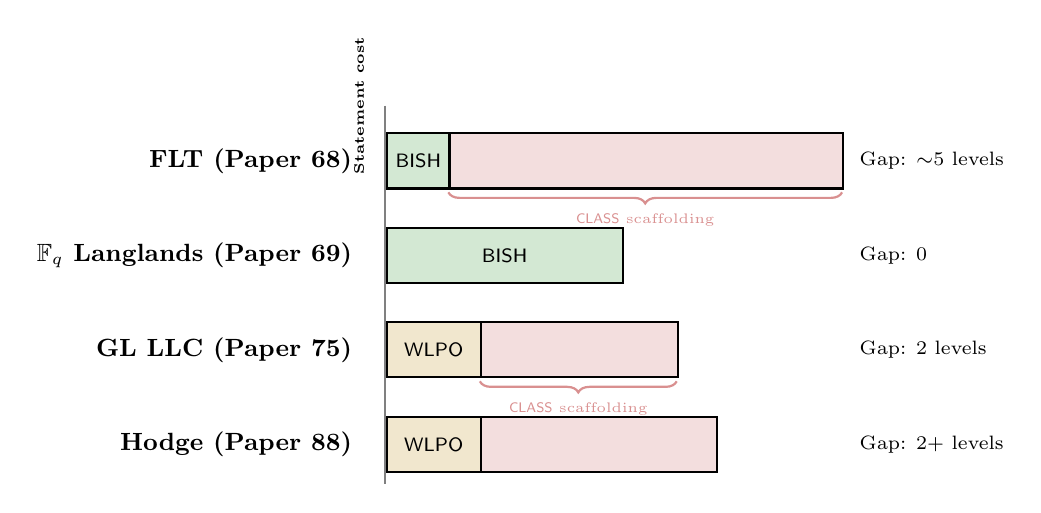
\begin{tikzpicture}[
  bar/.style={draw, thick, minimum height=0.7cm, align=center, font=\scriptsize},
  node distance=0.15cm
]
  % FLT
  \node[font=\small\bfseries, anchor=east] at (-0.3, 3) {FLT (\paperref{68})};
  \node[bar, fill=bishgreen!20, minimum width=0.8cm, anchor=west] at (0, 3) {\BISH};
  \node[bar, fill=classred!15, minimum width=5cm, anchor=west] at (0.8, 3) {};
  \node[font=\scriptsize, anchor=west] at (5.9, 3) {Gap: ${\sim}$5 levels};
  \draw[decorate, decoration={brace, amplitude=4pt, mirror}, thick, classred!50]
    (0.8, 2.6) -- (5.8, 2.6) node[midway, below=4pt, font=\tiny] {\CLASS{} scaffolding};

  % Function field Langlands
  \node[font=\small\bfseries, anchor=east] at (-0.3, 1.8) {$\mathbb{F}_q$ Langlands (\paperref{69})};
  \node[bar, fill=bishgreen!20, minimum width=3cm, anchor=west] at (0, 1.8) {\BISH};
  \node[font=\scriptsize, anchor=west] at (5.9, 1.8) {Gap: 0};

  % GL LLC
  \node[font=\small\bfseries, anchor=east] at (-0.3, 0.6) {GL LLC (\paperref{75})};
  \node[bar, fill=wlpogold!20, minimum width=1.2cm, anchor=west] at (0, 0.6) {\WLPO};
  \node[bar, fill=classred!15, minimum width=2.5cm, anchor=west] at (1.2, 0.6) {};
  \node[font=\scriptsize, anchor=west] at (5.9, 0.6) {Gap: 2 levels};
  \draw[decorate, decoration={brace, amplitude=4pt, mirror}, thick, classred!50]
    (1.2, 0.2) -- (3.7, 0.2) node[midway, below=4pt, font=\tiny] {\CLASS{} scaffolding};

  % Hodge
  \node[font=\small\bfseries, anchor=east] at (-0.3, -0.6) {Hodge (\paperref{88})};
  \node[bar, fill=wlpogold!20, minimum width=1.2cm, anchor=west] at (0, -0.6) {\WLPO};
  \node[bar, fill=classred!15, minimum width=3cm, anchor=west] at (1.2, -0.6) {};
  \node[font=\scriptsize, anchor=west] at (5.9, -0.6) {Gap: 2+ levels};

  % Statement vs Proof labels
  \draw[thick, gray] (0, 3.7) -- (0, -1.1);
  \node[above, font=\tiny\bfseries, rotate=90] at (-0.15, 3.7) {Statement cost};
\end{tikzpicture}
\caption{Conservation gaps: the difference between what a theorem \emph{states} (left edge) and what its proof \emph{costs} (right edge). A gap of zero means the proof is optimal. A large gap suggests a simpler proof may exist. Decreasing gaps correlate with increasing algebraicity.}
\label{fig:conservation-gap}
\end{figure}

CRM-trained AI uses conservation gap data as a training signal: large gaps predict where constructive alternatives exist, guiding automated proof search toward simpler proofs.


%══════════════════════════════════════════════════════════
% CHAPTER 4
%══════════════════════════════════════════════════════════
\chapter{The Squeeze Protocol}

Chapters 1--3 were diagnosis: what does mathematics cost? This chapter is the \emph{instrument}---the automated tool that performs the diagnosis. It transforms CRM from a manual audit into a systematic, repeatable protocol.

\begin{analogybox}[Chapter Preview: The X-Ray Machine]
Imagine a doctor (CRM) who has been diagnosing diseases (logical cost) by hand---examining each patient (theorem) one at a time. Now the doctor builds an X-ray machine (CRMLint) that can scan any patient automatically and produce a precise map: this bone is healthy (constructive), this bone is fractured (classical).

The Squeeze protocol is the full procedure: (1) position the patient (scaffold the proof in Lean~4), (2) take the X-ray (trace classical dependencies), (3) mark the fractures (identify Classical Boundary Nodes), (4) set the bones (replace classical steps with constructive alternatives where possible).
\end{analogybox}


%── 4.1 ───────────────────────────────────────────────────
\section{CRMLint: The Automated Analyzer}

\paperref{76} introduces CRMLint (940 lines Lean~4, zero \texttt{sorry}). CRMLint is a \emph{metaprogram}---a program that analyzes other programs. Think of it as a code analysis tool (like a linter for Python or JavaScript) but instead of checking style, it checks \emph{logical cost}. It takes a Lean~4 proof term, traces the classical dependency graph, and reports exactly which steps require non-constructive principles.

CRMLint operates in four layers:

\begin{enumerate}
  \item \textbf{Classical dependency tracer.} Walk the proof term DAG (directed acyclic graph). Flag every node where \texttt{Classical.choice} or equivalent enters.
  \item \textbf{Pattern classifier.} Categorize each flagged node: is it analytic continuation? Zariski density? Ehresmann fibration? Hodge decomposition?
  \item \textbf{Concentration analyzer.} Measure what fraction of the proof is \BISH{} vs.\ \CLASS.
  \item \textbf{Audit reporter.} Emit a structured decomposition: $n$ \BISH{} components + $m$ \CLASS{} components = total.
\end{enumerate}

\textbf{Key distinction:} CRMLint measures \emph{logical cost}, not \emph{proof complexity}. Taylor-Wiles patching is complex but \BISH. Weight-1 modular forms are routine but \WLPO. This distinction is invisible without CRM.


%── 4.2 ───────────────────────────────────────────────────
\section{The Four-Step Squeeze Protocol}

\begin{figure}[htbp]
\centering
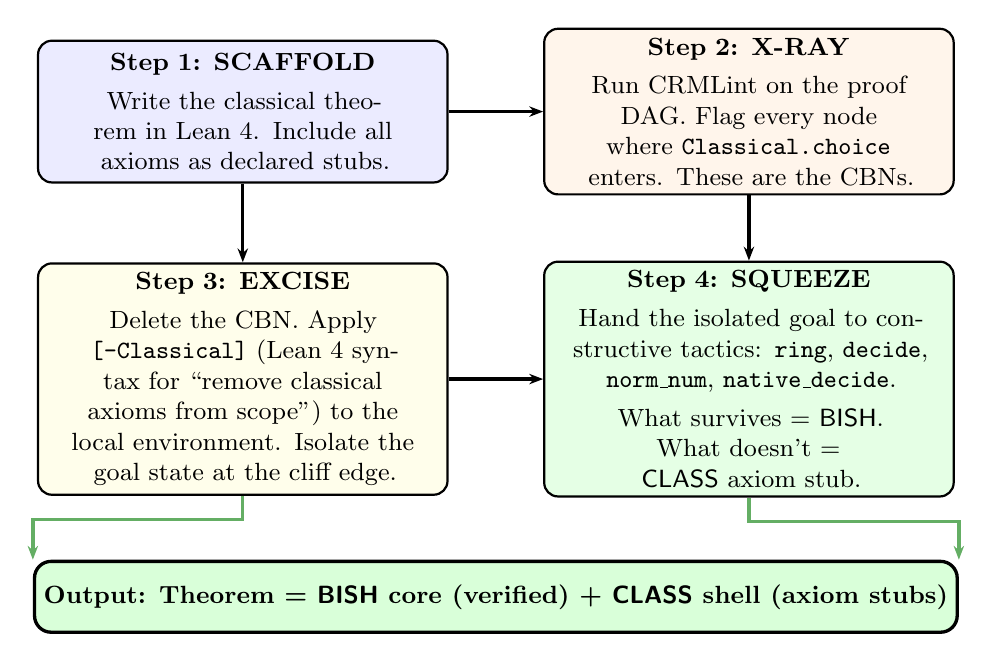
\begin{tikzpicture}[
  sbox/.style={draw, rounded corners=5pt, thick,
    minimum width=5.2cm, minimum height=1.8cm,
    align=center, font=\small, text width=4.8cm},
  node distance=0.6cm and 1.2cm
]
  % Step 1
  \node[sbox, fill=blue!8] (s1) {
    \textbf{Step 1: SCAFFOLD}\\[3pt]
    Write the classical theorem in Lean~4.
    Include all axioms as declared stubs.
  };
  % Step 2
  \node[sbox, fill=orange!8, right=of s1] (s2) {
    \textbf{Step 2: X-RAY}\\[3pt]
    Run CRMLint on the proof DAG.
    Flag every node where \texttt{Classical.choice} enters.
    These are the CBNs.
  };
  % Step 3
  \node[sbox, fill=yellow!8, below=1cm of s1] (s3) {
    \textbf{Step 3: EXCISE}\\[3pt]
    Delete the CBN.
    Apply \texttt{[-Classical]} (Lean~4 syntax for ``remove classical axioms from scope'') to the local environment.
    Isolate the goal state at the cliff edge.
  };
  % Step 4
  \node[sbox, fill=green!10, right=of s3] (s4) {
    \textbf{Step 4: SQUEEZE}\\[3pt]
    Hand the isolated goal to constructive tactics:
    \texttt{ring}, \texttt{decide}, \texttt{norm\_num},
    \texttt{native\_decide}.\\[3pt]
    What survives = \BISH.\\
    What doesn't = \CLASS{} axiom stub.
  };

  % Arrows
  \draw[arr, very thick] (s1) -- (s2);
  \draw[arr, very thick] (s2) -- (s4);
  \draw[arr, very thick] (s1) -- (s3);
  \draw[arr, very thick] (s3) -- (s4);

  % Result
  \node[draw, very thick, rounded corners=6pt,
        fill=green!15, minimum width=10cm,
        minimum height=0.9cm, below=0.8cm of $(s3.south)!0.5!(s4.south)$,
        font=\small\bfseries] (result)
    {Output: Theorem = \BISH{} core (verified) + \CLASS{} shell (axiom stubs)};
  \draw[arr, very thick, bishgreen!70] (s3.south) -- ++(0,-0.3) -| (result.north west);
  \draw[arr, very thick, bishgreen!70] (s4.south) -- ++(0,-0.3) -| (result.north east);
\end{tikzpicture}
\caption{The four-step Squeeze protocol. A classical proof is scaffolded, X-rayed for classical dependency nodes, excised at the boundary, and squeezed with constructive tactics. Typically $>$80\% of the formal content survives as \BISH.}
\label{fig:squeeze-protocol}
\end{figure}

\textbf{CBN} = \textbf{Classical Boundary Node}: the exact point where the proof jumps from computation to oracle. Key intuition: classical mathematics uses infinity as a compression algorithm. The Squeeze bans the shortcut and forces explicit algebraic witness discovery.


%── 4.3 ───────────────────────────────────────────────────
\section{Asymmetric Offloading}

The Squeeze exploits a division of labor between a \textbf{Computer Algebra System} (CAS)---software like SymPy or SageMath that performs exact symbolic computation---and a \textbf{proof assistant} (Lean~4) that verifies the results. The CAS computes; Lean certifies. Neither trusts the other: the CAS may have bugs, but Lean checks every identity independently.

\begin{table}[htbp]
\centering\small
\caption{Development time comparison across the program.}
\label{tab:offloading}
\renewcommand{\arraystretch}{1.2}
\begin{tabular}{@{}l l l l@{}}
\toprule
\textbf{Paper} & \textbf{Method} & \textbf{Density} & \textbf{Time} \\
\midrule
\paperref{5} (2024) & Manual Lean & $\sim$200 lines & 4 months \\
\paperref{77} (2026) & CAS + Lean pipeline & $\sim$798 lines & 1 hour \\
\bottomrule
\end{tabular}
\end{table}

A 2,900$\times$ speedup. \paperref{80} upgraded from \texttt{native\_decide} on concrete rationals to \texttt{ring} on polynomial rings $\mathbb{Q}[x,t]$---from retail auditing (one number at a time) to wholesale auditing (identities over entire polynomial rings). All subsequent Squeeze applications use \texttt{ring} over polynomial rings.


%── 4.4 ───────────────────────────────────────────────────
\section{The Function-Field Upgrade: Retail to Wholesale}

\paperref{80} introduced an infrastructure breakthrough that enabled all subsequent Squeeze applications.

\paperref{77--78} verified identities at \textbf{concrete rational numbers} using \texttt{native\_decide} (``is $7 \times 3 = 21$? Yes''). This checks one point at a time. To verify an identity across an entire family of varieties, you would need infinitely many checks.

\paperref{80} upgraded to \textbf{polynomial rings} using \texttt{ring} (``is this identity in $\mathbb{Q}[x,t]$ true? Yes''). This checks an entire family at once. A single \texttt{ring} invocation verifies a polynomial identity over all specializations simultaneously.

\begin{analogybox}[Analogy: retail vs.\ wholesale]
\texttt{native\_decide} is retail auditing: checking one house at a time. \texttt{ring} over $\mathbb{Q}(t)$ is wholesale auditing: mapping the entire neighborhood at once. Instead of checking one fiber of a family ($C_t$ at $t = 7$), you verify the whole family ($C_t$ for all $t$) in a single computation.
\end{analogybox}

This upgrade---from $\mathbb{Q}$-arithmetic to $\mathbb{Q}(t)$-algebra---is what makes the Hodge and BSD campaigns feasible. All subsequent Squeeze applications (\paperref{81--89, 92--96}) use \texttt{ring} over polynomial rings as their primary verification tactic.

The oracle content is also clarified by this upgrade. Working over $\mathbb{Q}(t)$ means the Squeeze verifies algebraic identities that hold \emph{generically}---for all but finitely many values of $t$. No oracle is needed to check these: the \texttt{ring} tactic decides polynomial identity in finite time. The oracle enters only when you need to pass from the algebraic identity to a topological or analytic conclusion (e.g., ``the flat section persists across the entire moduli space''). This is the structural reason why detection is \BISH{} and existence is \CLASS: detection is algebra (decidable by \texttt{ring}), existence is topology (requires an oracle).


%── 4.5 ───────────────────────────────────────────────────
\section{What Classical Boundary Nodes Look Like}

\begin{table}[htbp]
\centering\small
\caption{Catalogue of Classical Boundary Nodes across the Squeeze applications. The pattern: \CLASS{} nodes are topological existence assertions; \BISH{} nodes are algebraic computations.}
\label{tab:cbn-types}
\renewcommand{\arraystretch}{1.15}
\begin{tabular}{@{}l l l@{}}
\toprule
\textbf{CBN Type} & \textbf{Papers} & \textbf{Principle} \\
\midrule
\rowcolor{red!6}
Analytic continuation & \paperref{80, 95} & \CLASS \\
\rowcolor{red!6}
Ehresmann fibration theorem & \paperref{80--81, 93} & \CLASS \\
\rowcolor{red!6}
Hodge decomposition (existence) & \paperref{84--89} & \CLASS \\
\rowcolor{red!6}
Variational Hodge Conjecture & \paperref{88--89} & \CLASS \\
\rowcolor{red!6}
Abel-Jacobi map / Baire category & \paperref{94} & \CLASS \\
\rowcolor{red!6}
Kolyvagin Euler system & \paperref{95} & \CLASS \\
\rowcolor{red!6}
Chebotarev density theorem & \paperref{95} & \CLASS \\
\rowcolor{red!6}
Cassels-Poitou-Tate duality & \paperref{95} & \CLASS \\
\rowcolor{red!6}
Zariski density & \paperref{82} & \CLASS \\
\bottomrule
\end{tabular}
\end{table}

\textbf{Guide to the CBN types above.} \emph{Analytic continuation}: extending a function beyond its natural domain of convergence, requiring limits over $\mathbb{R}$. \emph{Ehresmann fibration}: a theorem guaranteeing that a smooth map with compact fibers is locally trivial---a topological existence result. \emph{Chebotarev density}: the existence of primes with prescribed splitting behaviour, proved via $L$-function analysis on $\mathbb{R}$. \emph{Cassels--Poitou--Tate duality}: a nine-term exact sequence assembling local Galois cohomology data at all primes simultaneously, requiring an infinite product.

\begin{thesisbox}[The Universal Pattern]
\CLASS{} nodes are always \textbf{topological existence} assertions: ``something exists in a topological space, but I cannot construct it.''
\BISH{} nodes are always \textbf{algebraic computations}: ``here is the explicit polynomial identity / matrix entry / eigenvalue / intersection number.''
The boundary is always: ``something exists'' vs.\ ``here it is.''
\end{thesisbox}


\subsection*{The Fifteen Applications at a Glance}

Table~\ref{tab:fifteen-apps} consolidates all fifteen Squeeze applications across the program. The progression reveals five phases: methodology (\paperref{77--78}), infrastructure (\paperref{80--83}), Hodge campaign (\paperref{84--89}), completion (\paperref{92--94}), and BSD campaign (\paperref{95--96}).

\begin{table}[htbp]
\centering\small
\caption{The fifteen CRMLint Squeeze applications (\paperref{90}, Table 1). For each application: the domain, what the Squeeze found to be constructive (\BISH{} core), what remains irreducibly classical (\CLASS{} boundary), and the Lean tactic that certifies the \BISH{} content.}
\label{tab:fifteen-apps}
\renewcommand{\arraystretch}{1.15}
\resizebox{\textwidth}{!}{%
\begin{tabular}{@{}c l l p{3.2cm} p{3cm} l@{}}
\toprule
\# & \textbf{Paper} & \textbf{Domain} & \textbf{\BISH{} Core} & \textbf{\CLASS{} Boundary} & \textbf{Tactic} \\
\midrule
\rowcolor{green!4}
1 & P77 & Hodge theory & 36 basis vectors for $\Hdg^{2,2}(E^4)$ & Lefschetz $(1,1)$ & \texttt{native\_decide} \\
2 & P78 & Langlands & Character-trace matching, $\GL_2(\mathbb{Q}_2)$ & Harris-Taylor & \texttt{decide} \\
\rowcolor{green!4}
3 & P80 & Algebraic GM & Griffiths pole reduction over $\mathbb{Q}(t)$ & Ehresmann-GM & \texttt{ring} \\
4 & P81 & Flat sections & Kronecker sum, symplectic flatness & Deligne monodromy & \texttt{ring} \\
\rowcolor{green!4}
5 & P82 & Diff.\ Galois & Kovacic's algorithm, $G_{\mathrm{gal}} = \SL_2$ & Zariski density & \texttt{norm\_num} \\
6 & P83 & Picard number & K\"unneth + flat dim + Kovacic $\to$ $\rho = 3$ & Noether-Lefschetz & \texttt{decide} \\
\rowcolor{green!4}
7 & P84 & Exotic Weil & Block GM, $G_{\mathrm{gal}}(\bigwedge^4 V_+) = \{1\}$ & Hodge existence & \texttt{ring} \\
8 & P85 & Exotic Weil & $\tau_+(t) = 0$, Lagrangian eigenspace & Hodge existence & \texttt{ring} \\
\rowcolor{green!4}
9 & P86 & Hodge Conj. & $D_8$-splitting, $\Jac \sim A^2$ & Ribet & \texttt{ring} \\
10 & P88 & Hodge Conj. & Fermat domination, $C_0 \to F_{16}$ & Shioda + VHC & \texttt{ring} \\
\rowcolor{green!4}
11 & P89 & Hodge Conj. & 18 components, $\tau_+(a,b,c) = 0$ & Shioda + VHC & \texttt{ring} \\
12 & P92 & Higher genus & $\tau_+(a) = 0$, genera 5--8 & Shioda + VHC & \texttt{ring}/\texttt{norm\_num} \\
\rowcolor{green!4}
13 & P94 & CY3 Griffiths & PF algebra, $\delta(z) \neq 0$ & Abel-Jacobi, Baire & \texttt{ring} \\
14 & P95 & BSD (rank 1) & Hecke eigenvalues, 2-descent, heights & Gross-Zagier, Kolyvagin & \texttt{native\_decide} \\
\rowcolor{green!4}
15 & P96 & BSD (rank 0) & Modular symbols, $L(E,1)/\Omega^+$, Tamagawa & Euler system, Iwasawa & \texttt{norm\_num} \\
\bottomrule
\end{tabular}%
}% end resizebox
\end{table}

\begin{remark}
Papers 87 and 91 appear in the generative arc but are \emph{not} Squeeze applications. Paper~87 is a foundational CRM analysis of the Hodge condition itself (its \WLPO{} equivalence is a calibration result). Paper~91 is a CRM audit of an external result (Markman's unconditional Hodge proof), comparing its logical cost with the Squeeze's. Paper~93 is a structural explanation (why $\tau_+ = 0$), not a decomposition.
\end{remark}


%── 4.5 ───────────────────────────────────────────────────
\section{The Gauss-Manin Pipeline}

\paperref{80--83} built the infrastructure for all subsequent Squeeze applications. This four-paper arc constructs the algebraic machinery needed to work with families of algebraic curves---the raw material for the Hodge campaign.

\begin{figure}[htbp]
\centering
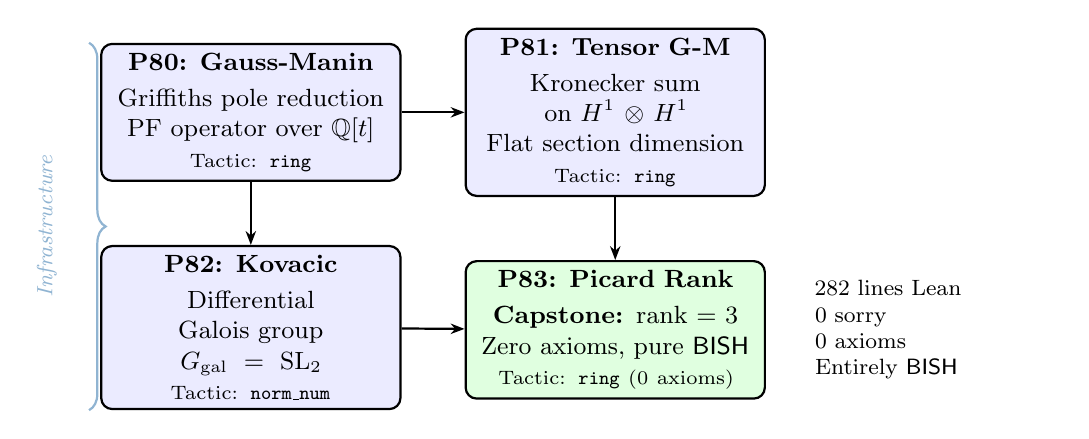
\begin{tikzpicture}[
  pbox/.style={draw, rounded corners=4pt, thick,
    minimum width=3.8cm, minimum height=1.5cm,
    align=center, font=\small, text width=3.4cm},
  node distance=0.8cm
]
  % P80
  \node[pbox, fill=blue!8] (p80) {
    \textbf{P80: Gauss-Manin}\\[2pt]
    Griffiths pole reduction\\
    PF operator over $\mathbb{Q}[t]$\\
    {\scriptsize Tactic: \texttt{ring}}
  };
  % P81
  \node[pbox, fill=blue!8, right=of p80] (p81) {
    \textbf{P81: Tensor G-M}\\[2pt]
    Kronecker sum on $H^1 \otimes H^1$\\
    Flat section dimension\\
    {\scriptsize Tactic: \texttt{ring}}
  };
  % P82
  \node[pbox, fill=blue!8, below=of p80] (p82) {
    \textbf{P82: Kovacic}\\[2pt]
    Differential Galois group\\
    $G_{\mathrm{gal}} = \mathrm{SL}_2$\\
    {\scriptsize Tactic: \texttt{norm\_num}}
  };
  % P83
  \node[pbox, fill=green!12, below=of p81] (p83) {
    \textbf{P83: Picard Rank}\\[2pt]
    \textbf{Capstone:} rank = 3\\
    Zero axioms, pure \BISH\\
    {\scriptsize Tactic: \texttt{ring} (0 axioms)}
  };

  % Arrows
  \draw[arr] (p80) -- (p81);
  \draw[arr] (p80) -- (p82);
  \draw[arr] (p81) -- (p83);
  \draw[arr] (p82) -- (p83);

  % Labels
  \draw[decorate, decoration={brace, amplitude=6pt},
        thick, bridgeblue!60]
    ([xshift=-4pt]p80.north west) -- ([xshift=-4pt]p82.south west)
    node[midway, left=8pt, font=\footnotesize\itshape, rotate=90, anchor=south]
      {Infrastructure};
  \node[right=0.5cm of p83, font=\footnotesize, text width=3cm, align=left]
    {282 lines Lean\\0 sorry\\0 axioms\\Entirely \BISH};
\end{tikzpicture}
\caption{The Gauss-Manin pipeline (\paperref{80--83}). P80 builds the Picard-Fuchs operator; P81 extends to tensor products; P82 determines the differential Galois group; P83 synthesizes into the Picard rank result---entirely \BISH{} with zero axioms.}
\label{fig:gauss-manin}
\end{figure}


%── 4.6 ───────────────────────────────────────────────────
\section{What Is a Picard-Fuchs Operator?}

\begin{analogybox}[Intuition First: The Shape-Tracker ODE]
Imagine a family of rubber bands, each a different shape, indexed by a dial $t$. As you turn the dial, the rubber band deforms continuously. The \emph{area enclosed} by the rubber band changes with $t$.

The Picard-Fuchs equation is the differential equation that describes \emph{how the area changes as you turn the dial}. It captures the deformation of the shape in a single algebraic formula. Crucially, the equation itself uses only rational functions of $t$---no actual integration, no topology, no $\mathbb{R}$. The equation is purely algebraic (\BISH), even though the areas it describes involve integrals (\CLASS).

This is why the Picard-Fuchs operator is the engine of the Squeeze: it replaces expensive topological integrals with cheap algebraic differential equations.
\end{analogybox}

A family of algebraic curves $C_t$ (parameterized by $t$) has cohomology that \emph{varies} with $t$. The \textbf{Picard-Fuchs equation} is the ODE satisfied by the \emph{periods}---integrals of differential forms over cycles:
\[
  \omega(t) = \int_\gamma \omega_t
\]
where $\gamma$ is a locally constant cycle and $\omega_t$ is an algebraic differential form on $C_t$.

\textbf{Example.} The Legendre family of elliptic curves $y^2 = x(x-1)(x-t)$ has Picard-Fuchs equation:
\[
  t(1-t)\,\omega''(t) + (1-2t)\,\omega'(t) - \tfrac{1}{4}\,\omega(t) = 0
\]
Its solution is the complete elliptic integral $K(t) = {}_2F_1(1/2, 1/2; 1; t)$.

\textbf{Why this matters for CRM.} The Picard-Fuchs operator encodes all the variation of the cohomology in a single algebraic ODE. Its coefficients are rational functions over $\mathbb{Q}(t)$---no topology, no $\mathbb{R}$, purely algebraic. This is the engine of the Squeeze: replace topological period integrals (cost \CLASS) with the algebraic PF operator (cost \BISH).


%── 4.7 ───────────────────────────────────────────────────
\section{Griffiths Transversality and Flat Sections}

\begin{analogybox}[Intuition: Parallel Transport Without Moving]
Imagine carrying a compass needle along a curved surface (like a sphere). The needle's direction changes as you walk---this change is the ``connection.'' A \textbf{flat section} is a direction that \emph{doesn't rotate} no matter which path you take. On a flat table, every direction is flat. On a sphere, no direction is globally flat (this is why the compass ``rotates'' when you walk around the North Pole).

In the Hodge campaign, the ``surface'' is the parameter space of a family of curves, the ``needle'' is a cohomology class, and the ``connection'' is the Gauss-Manin connection. A flat section is a cohomology class that stays constant across the entire family---the key ingredient for proving the Hodge conjecture.

The miracle: the connection matrix $M(t)$ has coefficients in $\mathbb{Q}(t)$---rational functions. So testing whether a section is flat ($M(t) \cdot v = 0$) is polynomial algebra, decidable by \texttt{ring}. No integrals needed.
\end{analogybox}

How do you compute the Picard-Fuchs operator without doing any integrals? The answer is \textbf{Griffiths pole reduction} (\paperref{80}).

\textbf{The Gauss-Manin connection.} Algebraic de~Rham cohomology $H^1_{\mathrm{dR}}(C_t/\mathbb{Q}(t))$ has a basis of algebraic differential forms. The Gauss-Manin connection $\nabla = d/dt + M(t)$ is a matrix ODE with rational function entries $M(t) \in M_{2\times 2}(\mathbb{Q}(t))$.

\textbf{Griffiths pole reduction.} Differentiating a basis form with respect to $t$ produces a meromorphic form with higher-order poles. Two algebraic identities reduce these poles:
\begin{enumerate}
  \item \textbf{Griffiths division:} $3(x^2 - x) = f'(x) + \bigl((2t-1)x - t\bigr)$ (removes exact components).
  \item \textbf{Coboundary identity:} $t(1-t)(x^2-x) = (3x+t-2)f(x) - (x^2-x)f'(x)$ (completes pole reduction).
\end{enumerate}
Both are \emph{polynomial identities over $\mathbb{Q}[x,t]$}, verified by Lean's \texttt{ring} tactic in milliseconds. No analysis. No limits. No $\mathbb{R}$.

\textbf{Griffiths transversality.} The connection preserves the cup-product pairing on de Rham cohomology. This forces the connection matrix $M$ to be traceless: $\mathrm{tr}(M) = 0$. Tracelessness is again a polynomial identity, verified by \texttt{ring}. This constraint is what makes the differential Galois group $\mathrm{SL}_2$ rather than $\mathrm{GL}_2$---a structural consequence that propagates through the entire Hodge campaign.

\textbf{Flat sections.} A \textbf{flat section} is a vector $v$ satisfying $\nabla(v) = 0$, i.e., $M(t) \cdot v = 0$ for all $t$. Flat sections are cohomology classes preserved under parallel transport along the family. The dimension of the flat section space determines the Picard number (\paperref{83}: dimension = 1, so generic Picard rank of $E_t \times E_t$ is 3). The trace form $\tau_+ = \mathrm{tr}(M_+)$ of the eigenspace connection measures whether an exotic Weil class is flat (\paperref{85}: $\tau_+ = 0$ universally).


\section{Diagnostic vs.\ Generative: Two Phases of the Programme}

The CRM program divides into two phases with fundamentally different characters. Table~\ref{tab:phase-comparison} contrasts them.

\begin{table}[htbp]
\centering\small
\caption{Diagnostic phase vs.\ generative phase (\paperref{90}, Table 2).}
\label{tab:phase-comparison}
\renewcommand{\arraystretch}{1.15}
\begin{tabular}{@{}l p{4.5cm} p{4.5cm}@{}}
\toprule
\textbf{Aspect} & \textbf{Diagnostic (P1--75)} & \textbf{Generative (P76--96)} \\
\midrule
Method & Manual calibration & Squeeze protocol \\
Input & Classical theorem & Classical theorem + CAS \\
Output & Level in hierarchy & $T_{\BISH} \wedge T_{\CLASS}$ decomposition \\
Verification & Lean (hand-written) & Lean (CAS-generated) \\
Domains & Physics, arith.\ geometry & Hodge, Langlands, diff.\ Galois, CY3 \\
Ceiling finding & \LPO{} for physics & VHC for Hodge; Abel-Jacobi for CY3 \\
Key insight & Logical cost $=$ cost of $\mathbb{R}$ & Microscope is automatable \\
Papers & 75 & 18 (incl.\ P76, P87, P90, P91) \\
Lean lines & ${\sim}87{,}000$ & ${\sim}9{,}000+$ \\
\bottomrule
\end{tabular}
\end{table}

\begin{analogybox}[Analogy: Geological Survey vs.\ Core Drilling]
The diagnostic phase was like a geological survey---walking across the terrain, sampling rock types, mapping the landscape. It was \emph{extensive}: 75 papers covering physics, arithmetic geometry, and representation theory. It discovered the terrain's structure: the logical cost of mathematics is the logical cost of $\mathbb{R}$.

The generative phase is like core drilling---choosing specific sites and drilling deep. It is \emph{intensive}: 18 papers developing and applying a single methodology. It doesn't just measure the cost; it extracts the constructive content and leaves only the irreducible classical boundary. The same drill bit (the Squeeze protocol) works at every site, from Hodge theory to BSD to Calabi-Yau geometry.
\end{analogybox}


%══════════════════════════════════════════════════════════
% CHAPTER 5
%══════════════════════════════════════════════════════════
\chapter{The Hodge Campaign}

The Hodge conjecture is a Clay Millennium Problem. It asks whether certain cohomological shadows of geometric objects are themselves geometric. The program devoted ten papers (\paperref{84--93}) to squeezing this conjecture---the most sustained application of CRMLint in the series.


%── 5.1 ───────────────────────────────────────────────────
\section{The Hodge Conjecture Explained}

Every smooth projective algebraic variety $X$ over $\mathbb{C}$ has cohomology groups $H^{2k}(X, \mathbb{Q})$. Inside these groups live special elements called \textbf{Hodge classes}---classes of type $(k,k)$ in the Hodge decomposition.

The Hodge conjecture asserts: \emph{every Hodge class is a rational linear combination of algebraic cycles} (geometric subvarieties).

\begin{analogybox}[Analogy: The Photograph Test]
Imagine a photograph (the cohomology group). Some patterns in the photograph arise from physical objects in the scene (algebraic cycles). Others might be lens artifacts or digital noise (non-algebraic classes). The Hodge conjecture says: every pattern that \emph{looks like} it comes from a physical object (Hodge class) \emph{actually does} come from a physical object (algebraic cycle). No lens artifacts.
\end{analogybox}


%── 5.2 ───────────────────────────────────────────────────
\section{The Hodge Horizon}

\paperref{87} established the CRM cost of the Hodge conjecture. Two key concepts here---\textbf{CM type} (complex multiplication metadata, defined in \S2.7) and \textbf{Mumford-Tate group} (the algebraic group controlling Hodge classes, defined below in \S5.3)---provide the algebraic shortcuts that reduce the cost:

\begin{figure}[htbp]
\centering
\resizebox{0.95\textwidth}{!}{%
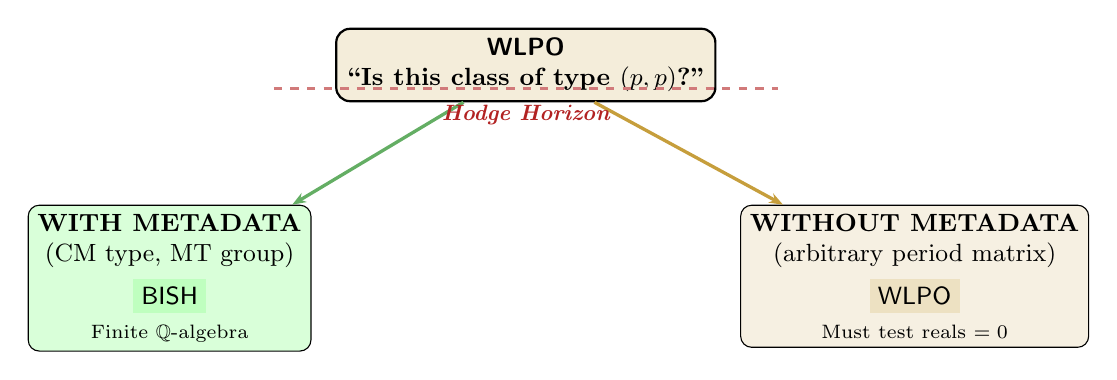
\begin{tikzpicture}[
  node distance=1.2cm and 2cm
]
  % Top: WLPO test
  \node[draw, rounded corners=5pt, thick, fill=wlpogold!15,
        minimum width=4cm, minimum height=0.9cm,
        align=center, font=\small\bfseries] (top)
    {\WLPO\\``Is this class of type $(p,p)$?''};

  % Branch left: with metadata
  \node[draw, rounded corners=4pt, fill=green!15,
        minimum width=3cm, minimum height=1.3cm,
        align=center, font=\small,
        below left=1.3cm and 0.3cm of top] (left)
    {\textbf{WITH METADATA}\\
     (CM type, MT group)\\[3pt]
     \colorbox{green!25}{\BISH}\\[1pt]
     {\scriptsize Finite $\mathbb{Q}$-algebra}};

  % Branch right: without metadata
  \node[draw, rounded corners=4pt, fill=wlpogold!12,
        minimum width=3cm, minimum height=1.3cm,
        align=center, font=\small,
        below right=1.3cm and 0.3cm of top] (right)
    {\textbf{WITHOUT METADATA}\\
     (arbitrary period matrix)\\[3pt]
     \colorbox{wlpogold!25}{\WLPO}\\[1pt]
     {\scriptsize Must test reals $= 0$}};

  % Arrows
  \draw[arr, bishgreen!70, very thick] (top) -- (left);
  \draw[arr, wlpogold!80, very thick] (top) -- (right);

  % Horizon line
  \draw[very thick, dashed, classred!60]
    (-3.2, -0.3) -- (3.2, -0.3)
    node[midway, below=2pt, font=\footnotesize\itshape\bfseries, text=classred]
      {Hodge Horizon};
\end{tikzpicture}%
}% end resizebox
\caption{The Hodge Horizon (\paperref{87}). With CM/MT metadata: \BISH. Without: \WLPO.}
\label{fig:hodge-horizon}
\end{figure}


%── 5.3 ───────────────────────────────────────────────────
\section{The Hodge Arc Step by Step}

\begin{analogybox}[The big picture before the details]
Imagine a family of musical instruments, each parameterized by a tuning knob $t$. Each instrument produces a set of overtones (the cohomology). As you turn the knob, the overtones shift---but some combinations of overtones stay perfectly constant, no matter where the knob is set. These are the \textbf{flat sections}.

The Hodge campaign asks: when a flat overtone-combination ``looks algebraic'' (it satisfies the Hodge condition), is it \emph{really} algebraic (produced by an actual geometric subshape)?

The answer depends on the instrument's internal symmetry. If the instrument has a hidden mirror symmetry (palindromic polynomial), it splits into two identical sub-instruments. The symmetry forces algebraicity. If there is no mirror symmetry, algebraicity requires a harder argument (VHC).

The ten-paper arc below makes this precise. The key concepts:
\begin{itemize}
  \item \textbf{Flat section} $=$ an overtone that doesn't change when you turn the knob ($\nabla v = 0$). Think: a pitch that is \emph{independent} of tuning.
  \item \textbf{Trace vanishing} $\tau_+ = 0$ $=$ the overtone-combination has zero ``drift.'' Verified by polynomial algebra (\BISH).
  \item \textbf{Kani-Rosen splitting} $=$ the instrument splits into two identical halves. This forces the Hodge conjecture to be true (Ribet's theorem). Purely algebraic (\BISH).
  \item \textbf{VHC} $=$ if the overtone is algebraic at one tuning, it stays algebraic at all tunings. Classical (\CLASS).
\end{itemize}
\end{analogybox}

\textbf{A note before the details.} The next several pages describe ten papers in sequence. Each paper builds on the previous one, so they are presented in order. If the formal details feel dense, focus on the \emph{plain English} paragraphs (in italics)---they capture the essential idea of each paper. The formal statements are there for completeness, but the conceptual story is self-contained without them.

Ten papers trace a complete arc from infrastructure through computation to structural explanation.

\begin{figure}[htbp]
\centering
\resizebox{\textwidth}{!}{%
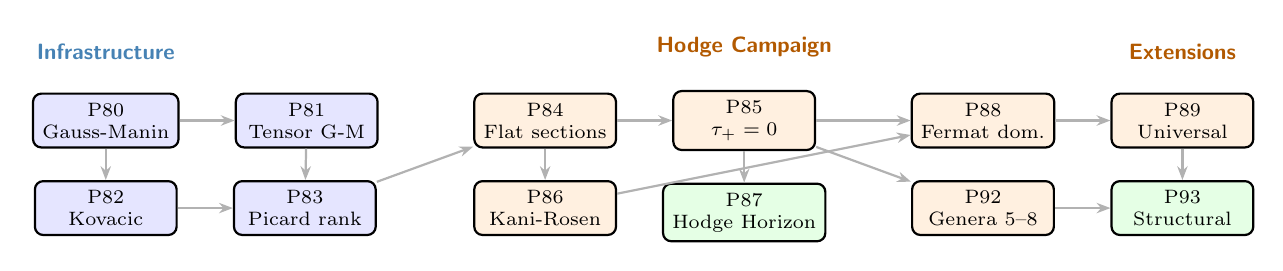
\begin{tikzpicture}[
  pnode/.style={draw, rounded corners=3pt, thick,
    minimum width=1.8cm, minimum height=0.6cm,
    align=center, font=\scriptsize},
  infra/.style={pnode, fill=blue!10},
  hodge/.style={pnode, fill=orange!12},
  cal/.style={pnode, fill=green!10},
  node distance=0.4cm and 0.7cm
]
  % Infrastructure arc
  \node[infra] (p80) {P80\\Gauss-Manin};
  \node[infra, right=of p80] (p81) {P81\\Tensor G-M};
  \node[infra, below=of p80] (p82) {P82\\Kovacic};
  \node[infra, right=of p82] (p83) {P83\\Picard rank};

  % Hodge campaign
  \node[hodge, right=1.2cm of p81] (p84) {P84\\Flat sections};
  \node[hodge, right=of p84] (p85) {P85\\$\tau_+=0$};
  \node[hodge, below=of p84] (p86) {P86\\Kani-Rosen};
  \node[cal, below=of p85] (p87) {P87\\Hodge Horizon};
  \node[hodge, right=1.2cm of p85] (p88) {P88\\Fermat dom.};
  \node[hodge, right=of p88] (p89) {P89\\Universal};
  \node[hodge, below=of p88] (p92) {P92\\Genera 5--8};
  \node[cal, below=of p89] (p93) {P93\\Structural};

  % Arrows
  \draw[arr, gray!60] (p80) -- (p81);
  \draw[arr, gray!60] (p80) -- (p82);
  \draw[arr, gray!60] (p81) -- (p83);
  \draw[arr, gray!60] (p82) -- (p83);
  \draw[arr, gray!60] (p83) -- (p84);
  \draw[arr, gray!60] (p84) -- (p85);
  \draw[arr, gray!60] (p84) -- (p86);
  \draw[arr, gray!60] (p85) -- (p87);
  \draw[arr, gray!60] (p85) -- (p88);
  \draw[arr, gray!60] (p86) -- (p88);
  \draw[arr, gray!60] (p88) -- (p89);
  \draw[arr, gray!60] (p85) -- (p92);
  \draw[arr, gray!60] (p89) -- (p93);
  \draw[arr, gray!60] (p92) -- (p93);

  % Labels
  \node[above=0.3cm of p80, font=\footnotesize\bfseries\sffamily,
        text=bridgeblue] {Infrastructure};
  \node[above=0.3cm of p85, font=\footnotesize\bfseries\sffamily,
        text=orange!70!black] {Hodge Campaign};
  \node[above=0.3cm of p89, font=\footnotesize\bfseries\sffamily,
        text=orange!70!black] {Extensions};
\end{tikzpicture}%
}% end resizebox
\caption{Dependency DAG for the Hodge campaign (\paperref{80--93}, from \paperref{90}). Blue = infrastructure, orange = campaign, green = calibration.}
\label{fig:hodge-dag}
\end{figure}

\subsection*{The arc in detail}

\textbf{P84: Exotic Weil classes as flat sections.}

\emph{The idea in plain English:} Take a curve with a 4-fold rotational symmetry ($\sigma$). This symmetry splits the cohomology into two pieces ($V_+$ and $V_-$), like splitting white light into two polarizations. Within $V_+$, there lives an ``exotic'' class---a Hodge class that doesn't come from the obvious geometric sources (divisors). The question: is it flat (constant across the family)?

The test family is the genus-4 hyperelliptic curve $C_t: y^2 = x^9 - tx^5 + x$. It has a $\mathbb{Z}/4\mathbb{Z}$-automorphism $\sigma(x,y) = (-x, iy)$, which splits the cohomology $H^1_{\mathrm{dR}}(C_t)$ into eigenspaces $V_+$ (eigenvalue $+i$) and $V_-$ (eigenvalue $-i$), each of dimension 2. This splitting is algebraic---it uses only the group action and linear algebra over $\mathbb{Q}(i)$, no analysis.

The Gauss-Manin connection restricts to block-diagonal form: $\nabla = \nabla_+ \oplus \nabla_-$ with separate connection matrices $M_+, M_-$ on each block. \paperref{82} showed $G_{\mathrm{gal}} = \mathrm{SL}_2$ for each block (Kovacic's algorithm). Since $\det(\mathrm{SL}_2) = 1$, the exterior power connection $\nabla_{\bigwedge^4 V_+}$ has trivial monodromy: $G_{\mathrm{gal}}(\bigwedge^4 V_+) = \{1\}$. This means the exotic Weil class $\omega \in \bigwedge^4 V_+$ is a \textbf{global flat section}---preserved under parallel transport. Entirely \BISH.

\emph{Translation:} The symmetry forces the exotic class to be constant. No oracle needed---just linear algebra.

\textbf{P85: Universal trace vanishing $\tau_+ = 0$.}

\emph{The idea in plain English:} The ``trace'' of the connection matrix measures how much the eigenspace $V_+$ rotates as you vary $t$. If $\tau_+ = 0$, the eigenspace doesn't rotate at all---the exotic class stays perfectly flat. This was verified computationally for every family tested, a universal phenomenon that cried out for structural explanation (which P93 eventually provided).

The trace form $\tau_+ = \mathrm{tr}(M_+)$ measures the ``twist'' of the eigenspace under variation. If $\tau_+ = 0$, the exotic Weil class is flat (parallel-transported without rotation). The eigenspace $V_+$ is \textbf{Lagrangian}: the symplectic intersection pairing restricted to $V_+$ vanishes, because the eigenvalues of $\sigma$ on $V_+$ and $V_-$ are $i$ and $-i$, and $i^2 = -1 \neq 1$. The symplectic constraint gives $\mathrm{tr}(M_+) = -\mathrm{tr}(M_-)$ but \emph{not} $\mathrm{tr}(M_+) = 0$ individually. Yet $\tau_+ = 0$ was verified computationally for every family tested (8 families across genera 2--5). A universal phenomenon demanding structural explanation.

\textbf{P86: Kani-Rosen splitting on the palindromic locus.}

\emph{The idea in plain English:} The polynomial defining the curve has a mirror symmetry: reading the coefficients left-to-right is the same as right-to-left (like ``racecar'' is a palindrome). This mirror symmetry produces a hidden involution on the curve, which together with the rotational symmetry generates a larger symmetry group ($D_8$, the symmetry group of a square). This forces the Jacobian to split into a product of two identical pieces---and for products of identical abelian surfaces, the Hodge conjecture is known unconditionally (Ribet 1983). No oracles, no open conjectures. Pure algebra.

The polynomial $g(x) = x^8 - tx^4 + 1$ is \textbf{palindromic}: the coefficient of $x^k$ equals the coefficient of $x^{8-k}$. This implies the existence of a \textbf{reciprocal involution} $\mu(x,y) = (1/x, y/x^5)$, satisfying $\mu^2 = \mathrm{id}$.

\textbf{The $D_8$ group.} The involution $\mu$ together with the order-4 automorphism $\sigma$ generates the dihedral group $D_8 = \langle \sigma, \mu \mid \sigma^4 = 1, \mu^2 = 1, \sigma\mu = \mu\sigma^3 \rangle$ of order 8. The relation $\sigma\mu = \mu\sigma^3$ is verified by direct coordinate computation.

\textbf{The splitting theorem.} The $D_8$-action produces two genus-2 quotient curves $Q_1 = C/\langle\mu\rangle$ and $Q_2 = C/\langle\mu\sigma^2\rangle$. The Kani-Rosen genus count $4 = 2 + 2 + 0 + 0$ gives the isogeny $J(C_t) \sim J(Q_1) \times J(Q_2)$. Over $\mathbb{C}$, $Q_1 \cong Q_2$ (via $(u,v) \mapsto (-u, iv)$), so $J(C_t) \sim A^2$ for an abelian surface $A = J(Q_1)$.

\textbf{Why $J(C_t) \sim A^2$ proves Hodge.} By Ribet's theorem (1983), the Hodge conjecture holds unconditionally for all powers of abelian surfaces---\emph{no hypothesis on $\mathrm{End}(A)$ or the Mumford-Tate group is needed.} Since $J(C_t) \sim A^2$, the exotic Weil class $\omega \in \bigwedge^4(V_+)$ is algebraic. \textbf{Unconditional.} 10 \BISH{} + 3 \CLASS{} = 77\% constructive.

\textbf{P87: The Hodge Horizon---Mumford-Tate and absolute Hodge classes.}
The \textbf{Mumford-Tate group} $\mathrm{MT}(A)$ measures ``how symmetric'' the Hodge structure of $A$ is. In plain terms: it is the smallest group of symmetries that is compatible with the Hodge decomposition. A large Mumford-Tate group (like the full symplectic group $\mathrm{GSp}_{2g}$) means the Hodge structure is ``generic''---no special symmetries. A small Mumford-Tate group means extra symmetries are present, and these extra symmetries provide the algebraic metadata that drops the Hodge test from \WLPO{} to \BISH.

Formally, $\mathrm{MT}(A)$ is the smallest $\mathbb{Q}$-algebraic subgroup of $\mathrm{GL}(H^1(A, \mathbb{Q}))$ whose base change to $\mathbb{R}$ contains the image of the Hodge cocharacter. The Hodge classes are precisely the $\mathrm{MT}(A)$-invariants: $\mathrm{Hdg}^p(A) = (\bigwedge^{2p} H^1(A,\mathbb{Q}))^{\mathrm{MT}(A)}$. For a generic abelian variety, $\mathrm{MT}(A) = \mathrm{GSp}_{2g}$, and the Hodge classes are the \emph{Lefschetz classes}---polynomials in the polarization class. Testing Lefschetz membership is finite $\mathbb{Q}$-linear algebra: \BISH.

Theorem~A: if $\mathrm{MT}(A)$ is known, the Hodge test is \BISH. Theorem~B: the \emph{uniform} Hodge test (a single algorithm for arbitrary period matrices) is $\Leftrightarrow$ \WLPO, because testing whether a real period integral equals zero requires the real-number equality oracle.

A Hodge class is \textbf{absolute Hodge} if it is stable under all automorphisms of $\mathbb{C}$. Deligne proved that all Hodge classes on abelian varieties are absolute Hodge. If the exotic Weil class could be shown to be absolute Hodge independently of VHC, algebraicity would follow from Deligne's framework---this is an open alternative to the Kani-Rosen approach for the generic complement.

\textbf{P88: Fermat domination and the Variational Hodge Conjecture (VHC).}

\emph{The idea in plain English:} When the palindromic symmetry is absent (coefficient $a \neq c$), the Jacobian doesn't split and the Kani-Rosen trick fails. Plan B: specialize to a single specific value ($t=0$) where the curve is dominated by the well-understood Fermat curve, prove the Hodge conjecture there (using Shioda's classical result), then invoke VHC to spread the answer to all $t$. VHC is the principle ``if it's algebraic at one point, it's algebraic everywhere''---a powerful but unproven statement (\CLASS).

On the \textbf{generic complement} $\{a \neq c\}$ (non-palindromic), the Jacobian $J(C_t)$ is simple---no Kani-Rosen splitting exists. \paperref{88} takes a different route: specialize to $t = 0$, where $C_0$ is dominated by the Fermat curve $F_{16}$. By Shioda's theorem, all Hodge classes on Fermat quotients are algebraic. So the exotic Weil class is algebraic at the special fiber $t = 0$.

The \textbf{Variational Hodge Conjecture} (Grothendieck, 1966) asserts: if a global flat section of the Gauss-Manin connection is algebraic at \emph{one} point $t_0$, it is algebraic at the generic point. VHC is open in general (it would follow from the Standard Conjectures). The proof chain is:
\[
  \tau_+ = 0 \;\xrightarrow{t=0}\; C_0 \to F_{16} \;\xrightarrow{\text{Shioda}}\; \omega|_{t=0} \text{ algebraic} \;\xrightarrow{\text{VHC}}\; \omega_\eta \text{ algebraic.}
\]
\textbf{Conditional} (VHC = \CLASS). This is the fundamental bifurcation: the palindromic locus gives unconditional algebraicity (Kani-Rosen, no VHC), while the generic complement requires VHC.

\textbf{P89: The universal 3-parameter family.}
Full family $C_{a,b,c}: y^2 = x^9 + ax^7 + bx^5 + cx^3 + x$. The trace form $\tau_+(a,b,c) = 0$ is verified for all three parameter directions ($\partial/\partial a$, $\partial/\partial b$, $\partial/\partial c$) as \emph{polynomial identities in $\mathbb{Z}[a,b,c]$}, checked by Lean's \texttt{ring} tactic. The palindromic locus $\{a = c\}$ is precisely the Kani-Rosen locus. This is the natural endpoint of the Griffiths + Fermat pipeline.

\subsection*{The 18/2 Ratio: Anatomy of the Hodge Conjecture}

Paper~89's universal squeeze yields the program's most striking quantitative finding: of the 20 logical components, 18 are \BISH{} and 2 are \CLASS. This 18/2 ratio is not accidental---it reflects the structural anatomy of the Hodge conjecture.

The 18 \BISH{} components decompose into three categories:
\begin{itemize}
  \item \textbf{Dimension data} (5 components): genus, $\dim H^1$, $\dim V_+$, $\dim \bigwedge^4 V_+$, base dimension. These are integers computed from the defining polynomial.
  \item \textbf{Symmetry data} (8 components): oddness, factorization, palindromic obstruction, palindromic at $a = c$, Fermat specialization, prior-paper specializations, non-palindromic core.  These are polynomial identities in $\mathbb{Z}[x,a,b,c]$.
  \item \textbf{Analytic data} (5 components): pullback bound, three $\tau_+$ vanishing identities (one per parameter direction), $\tau_-$ vanishing. These encode the trace of the Gauss-Manin connection restricted to eigenspaces.
\end{itemize}

The 2 \CLASS{} components are both \emph{existence assertions}:
\begin{enumerate}
  \item \textbf{Shioda:} there \emph{exists} an algebraic cycle representing the exotic Weil class at the Fermat point.
  \item \textbf{VHC:} there \emph{exists} an algebraic cycle representing the flat extension to the generic fiber.
\end{enumerate}

\begin{thesisbox}[The Pattern: Computation is \BISH; Existence is \CLASS]
Everything that can be computed from the defining polynomial is constructive. The only irreducible classical content is the assertion that a geometric object (an algebraic cycle) \emph{exists}. This pattern---detection is \BISH, existence is \CLASS---will prove universal across the entire program.
\end{thesisbox}


\textbf{P92: Zariski Grid Specialization for genera 5--8.}
For genera $\geq 6$, symbolic expansion of the Griffiths pole reduction triggers exponential intermediate expression swell---the B\'ezout identity coefficients have hundreds of terms, exhausting physical memory. \paperref{92} introduces \textbf{Zariski Grid Specialization}: evaluate $\tau_+$ at concrete integer fibers in $\mathbb{Q}[x]$ (where B\'ezout takes milliseconds), verify cancellation by \texttt{norm\_num}, then invoke the \textbf{Schwartz-Zippel lemma}: a nonzero polynomial $P \in \mathbb{Z}[x_1,\ldots,x_n]$ of total degree $\leq D$ has at most $D \cdot |S|^{n-1}$ zeros on any grid $S^n$. If $\tau_+$ vanishes at all $(D+1)^n$ grid points, it is identically zero. Both below the wall (genus $\leq 5$, \texttt{ring}) and above the wall (genus $\geq 6$, \texttt{norm\_num} + Schwartz-Zippel) are \BISH. The wall separates verification \emph{modalities}, not logical \emph{levels}.

A key parity observation emerges from this multi-genus analysis: for \textbf{odd} $g$, the exterior power $\bigwedge^g V_+$ lies in odd-degree cohomology $H^g(J(C), \mathbb{Q})$, and there are no Hodge classes in odd-degree cohomology (Hodge classes live in $H^{2k}$, even degree). So for odd $g$ the Hodge question is vacuous---there is no exotic class to worry about. The interesting case is always \textbf{even} $g$ (4, 6, 8,~\ldots), where VHC + Fermat anchor gives conditional algebraicity.

\textbf{P93: Structural Vanishing Theorem---why $\tau_+ = 0$ universally.}

\emph{The idea in plain English:} Papers 84--92 \emph{observed} that $\tau_+ = 0$ for every family tested. P93 \emph{explains why}. Two independent arguments, from different branches of mathematics, reach the same conclusion. The first (hypergeometric) shows that the oddness of the defining polynomial kills the discriminant, and the unit leading/trailing coefficients freeze the boundary terms. The second (topological) uses Deligne's regularity theory to force the vanishing globally.

Two independent proofs explain the computational miracle:

\textbf{Proof 1 (Varchenko hypergeometric).} The $\mathbb{Z}/4\mathbb{Z}$-action and the substitution $u = x^2$ transform $V_+$ into a twisted cohomology of a rank-1 local system on $\mathbb{P}^1$ punctured at the roots $u_1, \ldots, u_g$ of $P(u)$. The \textbf{Varchenko exponents} are:
\begin{itemize}
  \item Root-root: $e_{ij} = \alpha_i + \alpha_j + 1 = (-1/2) + (-1/2) + 1 = 0$.
  \item Origin-root: $e_{0i} = \alpha_0 + \alpha_i + 1 = (-3/4) + (-1/2) + 1 = -1/4$.
\end{itemize}
The root-root exponents are all zero, so the discriminant of $P(u)$ drops entirely out of the period determinant. Then \textbf{Vieta freezing}: for $P(u) = u^g + a_1 u^{g-1} + \cdots + 1$, Vieta's formulas give $\prod u_i = (-1)^g \cdot 1/1 = (-1)^g$---a fixed rational number independent of the parameters. So $\det(\Pi_+)$ is proportional to a constant, and $\tau_+ = d\log(\text{const}) = 0$. ``Oddness kills the discriminant; unit coefficients freeze the boundary.''

\textbf{Proof 2 (Deligne topological).} Deligne regularity guarantees $\tau_+$ has at most logarithmic poles. Picard-Lefschetz theory constrains the monodromy at each singular fiber. Together they force $\tau_+ = 0$ on the entire base. This proof is 4 \CLASS{} components (Deligne regularity and Picard-Lefschetz are topological existence theorems).

CRM decomposition: 13 \BISH{} + 4 \CLASS{}. Both proofs reach the same conclusion; the CRM audit shows the hypergeometric proof is cheaper.


%── 5.4 ───────────────────────────────────────────────────
\section{The Hodge Bifurcation}

\begin{analogybox}[The Fork in the Road]
Imagine walking through a landscape where the ``logical cost'' of the terrain changes abruptly. On one side of a wall ($a = c$, the palindromic locus), the ground is flat and easy to traverse (\BISH{}---the Kani-Rosen trick works, the Hodge conjecture is unconditional). On the other side ($a \neq c$), you need heavy equipment (\CLASS{}---VHC required).

The wall itself is infinitely thin (codimension~1 in parameter space), but the cost jumps discontinuously across it. A discrete algebraic property (palindromic symmetry) controls this jump. This is not accidental: the symmetry determines whether the Jacobian splits, which determines whether Ribet's theorem applies.
\end{analogybox}

The most striking finding of the Hodge campaign: a discrete invariant---palindromic symmetry---controls the CRM cost. The cost jumps discontinuously across a codimension-1 locus.

\begin{figure}[htbp]
\centering
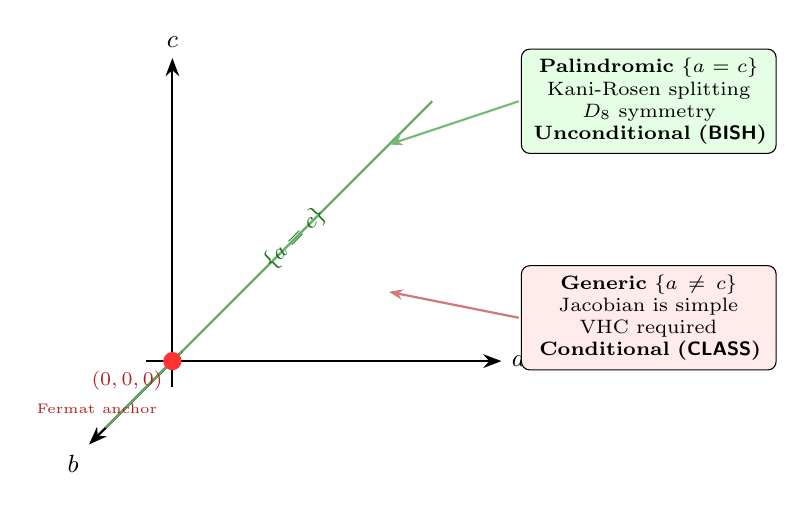
\begin{tikzpicture}[scale=1.1]
  % 3D axes
  \draw[-{Stealth}, thick] (-0.3,0,0) -- (3.8,0,0)
    node[right, font=\small] {$a$};
  \draw[-{Stealth}, thick] (0,-0.3,0) -- (0,3.5,0)
    node[above, font=\small] {$c$};
  \draw[-{Stealth}, thick] (0,0,-0.3) -- (0,0,2.5)
    node[below left, font=\small] {$b$};

  % Palindromic plane {a = c}
  \fill[bishgreen!15, opacity=0.6]
    (0,0,0) -- (3,3,0) -- (3,3,2) -- (0,0,2) -- cycle;
  \draw[thick, bishgreen!70]
    (0,0,0) -- (3,3,0) -- (3,3,2) -- (0,0,2) -- cycle;

  % Label on plane
  \node[font=\footnotesize\bfseries, text=bishgreen!80!black,
        rotate=45] at (1.8,1.8,1) {$\{a = c\}$};

  % Fermat point
  \fill[red!80] (0,0,0) circle (3pt);
  \node[below left, font=\scriptsize\bfseries, text=classred] at (0,0,0)
    {$(0,0,0)$};
  \node[below left=12pt and 2pt, font=\tiny, text=classred] at (0,0,0)
    {Fermat anchor};

  % Annotations
  \node[draw, rounded corners=3pt, fill=green!10,
        font=\scriptsize, text width=3cm, align=center]
    at (5.5, 3) {
    \textbf{Palindromic $\{a=c\}$}\\
    Kani-Rosen splitting\\
    $D_8$ symmetry\\
    \textbf{Unconditional (\BISH)}
  };
  \node[draw, rounded corners=3pt, fill=red!8,
        font=\scriptsize, text width=3cm, align=center]
    at (5.5, 0.5) {
    \textbf{Generic $\{a \neq c\}$}\\
    Jacobian is simple\\
    VHC required\\
    \textbf{Conditional (\CLASS)}
  };

  \draw[arr, bishgreen!60] (4, 3) -- (2.5, 2.5);
  \draw[arr, classred!60] (4, 0.5) -- (2.5, 0.8);
\end{tikzpicture}
\caption{The Hodge bifurcation in $\mathbb{A}^3_{\mathbb{Q}}$ (adapted from \paperref{90}). The palindromic locus $\{a=c\}$ has codimension~1 and gives unconditional algebraicity (\BISH{} via Kani-Rosen). The generic complement $\{a \neq c\}$ requires VHC (\CLASS). Cost jumps discontinuously.}
\label{fig:hodge-bifurcation}
\end{figure}


%── 5.5 ───────────────────────────────────────────────────
\section{The Markman Comparison}

\paperref{91} audited Markman's 2025 unconditional proof of the Hodge conjecture for certain hyper-K\"ahler manifolds (arXiv:2502.03415) alongside the CRMLint Squeeze results:

\begin{table}[htbp]
\centering\small
\caption{CRMLint Squeeze vs.\ Markman (2025): two approaches to Hodge algebraicity compared.}
\label{tab:markman}
\renewcommand{\arraystretch}{1.2}
\begin{tabular}{@{}l c c c c@{}}
\toprule
\textbf{Method} & \textbf{\BISH} & \textbf{\CLASS} & \textbf{Total} & \textbf{\% \BISH} \\
\midrule
\rowcolor{green!6}
CRMLint Squeeze (conditional on VHC) & 18 & 2 & 20 & 90\% \\
\rowcolor{red!4}
Markman (unconditional) & 4 & 5 & 9 & 44\% \\
\bottomrule
\end{tabular}
\end{table}

The Squeeze extracts more constructive content at finer granularity, but is conditional on VHC. Markman is unconditional but uses more classical machinery. Key finding: the cycle class map is irreducibly \CLASS{} (best achievable: 19/1).


\section{CRMLint as Discovery Instrument}

The Squeeze protocol is not merely an analysis tool---it is a \emph{discovery} tool. Three results in the Hodge campaign were found \emph{by} the Squeeze, not predicted by prior theory:

\begin{enumerate}
  \item \textbf{The trace vanishing $\tau_+ = 0$ (\paperref{85, 89}).} The CAS computed the Gauss-Manin connection matrix, extracted the trace on the $V_+$ eigenspace, and discovered it was identically zero. No theorem in the Hodge theory literature predicted this vanishing. It was a computational observation that demanded a structural explanation (later provided by \paperref{93}).

  \item \textbf{The palindromic obstruction (\paperref{89}).} The polynomial $g(x) - g_{\mathrm{rev}}(x) = (a - c)(x^6 - x^2)$ was found by the Squeeze pipeline. It reveals the \emph{precise polynomial} that controls the logical bifurcation between unconditional (Kani-Rosen, $a = c$) and conditional (VHC, $a \neq c$) results. The obstruction was invisible before the systematic parameter-space decomposition.

  \item \textbf{The hidden reciprocal involution (\paperref{86}).} The involution $\mu(x,y) = (1/x,\, y/x^5)$, whose $D_8$-action with the order-8 automorphism $\sigma$ was not previously noted in the literature for this family, was found by analyzing the palindromic symmetry through the Squeeze lens. Without the Squeeze's systematic decomposition of the $\mathbb{Q}(i)$-action on the Jacobian, this involution would likely have remained unnoticed.
\end{enumerate}

In each case, the protocol's systematic decomposition forced attention to structural features that ad hoc analysis would miss. The microscope is not passive: by banning classical shortcuts, it forces the prover to confront algebraic structures that classical proofs glide over.


\section{Connection to the Hodge Theory Literature}

\textbf{This section is for readers with algebraic geometry background.} It places the Hodge campaign in the context of prior work. Skip to \S5.8 if you prefer to continue the narrative.

The exotic Weil classes studied in the Hodge campaign are instances of a broader phenomenon in the Hodge theory of abelian varieties:

\begin{itemize}
  \item \textbf{Moonen-Zarhin (1999)} proved that for abelian varieties of dimension $\leq 5$, all Hodge classes are \emph{absolute Hodge}---stable under all automorphisms of $\mathbb{C}$. This does not prove algebraicity (absolute Hodge $\not\Rightarrow$ algebraic in general), but it eliminates one obstruction.

  \item \textbf{Van Geemen (2001)} classified the exotic Weil classes for abelian fourfolds with $\mathbb{Q}(i)$-action and showed that their algebraicity is genuinely open for simple abelian varieties with trivial endomorphism ring.

  \item The \textbf{Mumford-Tate conjecture}, if true, would imply that Hodge classes on abelian varieties are determined by the Mumford-Tate group. For fourfolds with $\mathbb{Q}(i)$-action, the generic $\mathrm{MT}$ is $\mathrm{GU}(4)$, and the invariant theory of $\mathrm{GU}(4)$ identifies the exotic Weil class as Hodge---but this does not prove it is algebraic.
\end{itemize}

The CRM contribution is orthogonal to these results. Where the classical literature asks ``is the exotic Weil class algebraic?'', CRM asks ``what is the \emph{logical cost} of asserting it is algebraic?'' The answer---\BISH{} for all computation, \CLASS{} only for the existence assertion---is new information that the classical framework cannot express. The 18/2 ratio, the palindromic bifurcation, and the trace vanishing are structural findings invisible to methods that do not distinguish constructive from classical content.


\section{Beyond Abelian Varieties: The Calabi-Yau Squeeze (\paperref{94})}

\begin{analogybox}[From Surfaces to Three-Dimensional Spaces]
The Hodge campaign (P84--93) studied abelian surfaces---two-dimensional objects where the exotic class lives in $H^4$ and the detection mechanism is trace vanishing ($\tau_+ = 0$). Paper~94 moves to a fundamentally different setting: a Calabi-Yau threefold (three-dimensional), where the interesting cohomology lives in $H^3$ (middle dimension) and the detection mechanism is entirely different---an \emph{infinitesimal invariant} $\delta(z) \neq 0$ coming from D-brane physics.

Think of it as testing the Squeeze protocol on a new kind of mountain, after having surveyed many hills.
\end{analogybox}

\textbf{The structural point first:} the detection/existence pattern (detection = \BISH, existence = \CLASS) persists even in a completely different geometric setting. The specific mechanisms change (trace vanishing becomes an infinitesimal invariant; VHC becomes the Abel--Jacobi map), but the logical architecture is identical. This universality is what the motivic framework (Chapter~7) explains.

The \textbf{mirror quintic} $X_\psi$ is the most studied Calabi-Yau threefold in physics---it is the mirror of the Fermat quintic $x_0^5 + x_1^5 + x_2^5 + x_3^5 + x_4^5 = 0$. Its \textbf{Griffiths group} $\mathrm{Griff}^2(X) = Z^2(X)_{\mathrm{hom}} / Z^2(X)_{\mathrm{alg}}$ measures algebraic cycles that are homologically trivial but not algebraically trivial---a subtler invariant than the Hodge question.

\textbf{Detection (\BISH).} The mirror quintic's periods satisfy a 4th-order Picard-Fuchs ODE. The \emph{domain wall tension}---a quantity from string theory measuring the tension of D-branes (higher-dimensional objects in string theory analogous to membranes) ending on $\mathbb{R}\mathbb{P}^3$---satisfies this ODE with a source term. The Walcher leading coefficient $b_0 = 30$ (30 holomorphic disks of minimal area) is computed by rational arithmetic and verified by \texttt{norm\_num}. The full recurrence $b_n = f(b_{n-1})$ is rational arithmetic over $\mathbb{Q}$, hence \BISH. Since $b_0 \neq 0$ and the recurrence multiplier is nonzero for all $n \geq 0$, induction gives $b_n \neq 0$ for all $n$---formally verified in Lean. This detects a non-trivial element of the Griffiths group: the infinitesimal invariant $\delta(z) \neq 0$.

\textbf{Existence (\CLASS).} The Abel-Jacobi map $\mathrm{AJ}: Z^2_{\mathrm{hom}}(X) \to J^2(X)$ requires integrating $(3,0)$-forms over 3-chains---period integrals involving limits and convergence (\CLASS). The infinite generation proof uses the \textbf{Baire Category Theorem}---the principle that a countable intersection of ``dense open'' sets in a complete metric space is still dense. Concretely: the space of Calabi--Yau threefolds where the Griffiths group is finitely generated is ``thin'' (meagre), so the ``generic'' CY3 has infinitely generated Griffiths group. This is an existence-by-genericity argument: it proves something exists without constructing it. Cost: \CLASS.

\textbf{Score: 11 \BISH{} + 3 \CLASS{} = 14 components (79\% constructive).} The \CLASS{} balance (3 nodes) is richer than the abelian surface setting (2 nodes: Shioda + VHC) because CY3 middle cohomology introduces the Abel-Jacobi and Baire obstructions. But the detection mechanism---the infinitesimal invariant $\delta \neq 0$ vs.\ the trace vanishing $\tau_+ = 0$---is structurally different yet equally \BISH.

This is where D-brane physics meets algebraic cycles: the CRM framework reveals that both programs share the same logical architecture (detection = \BISH, existence = \CLASS).


%══════════════════════════════════════════════════════════
% CHAPTER 6
%══════════════════════════════════════════════════════════
\chapter{The BSD Application}

The Birch and Swinnerton-Dyer conjecture (BSD) is the second Clay Millennium Problem audited by the program. Where the Hodge campaign squeezed cohomological detection, BSD squeezes $L$-function arithmetic.


%── 6.1 ───────────────────────────────────────────────────
\section{BSD Explained}

An \textbf{elliptic curve} $E$ over $\mathbb{Q}$ is a curve defined by an equation like $y^2 + y = x^3 - x$. The central question is: what is the \textbf{rank} of $E$---how many independent rational points does it have? (The \textbf{Mordell--Weil theorem} guarantees that the group of rational points $E(\mathbb{Q})$ is finitely generated, so the rank is a well-defined non-negative integer.)

The BSD conjecture connects this algebraic question to an analytic one: the rank equals the order of vanishing of the $L$-function $L(E,s)$ at $s = 1$. The Gross-Zagier theorem and Kolyvagin's Euler system prove BSD for rank 0 and rank 1 (conditional on modularity, which is now known).

The $L$-function $L(E,s)$ is built from local data: for each prime $p$ not dividing the conductor $N$, define $a_p = p + 1 - \#E(\mathbb{F}_p)$---the ``error term'' in the point count over the finite field $\mathbb{F}_p$. These are assembled into an Euler product $L(E,s) = \prod_p (1 - a_p p^{-s} + p^{1-2s})^{-1}$, which converges for $\mathrm{Re}(s) > 3/2$. The conjecture concerns the behaviour at $s = 1$, which lies \emph{outside the region of convergence}---this is why analytic continuation enters and why the Archimedean place is unavoidable.

\begin{analogybox}[Analogy: the census and the mirror]
Computing $a_p$ for each prime $p$ is like conducting a census: go door to door (finite field, finite count). This is \BISH. The BSD conjecture says that the \emph{aggregate pattern} of these census results, reflected in the behaviour of $L(E,s)$ at $s = 1$, encodes the global structure (rank). But reading this aggregate pattern requires \emph{analytic continuation}---extending the census data from ``where it converges'' to ``where it means something.'' That extension is the mirror: it passes through $\mathbb{R}$, and costs \CLASS.
\end{analogybox}


%── 6.2 Heegner Points ─────────────────────────────────────
\section{Heegner Points: Algebraic Points from CM Theory}

A \textbf{Heegner point} is a special algebraic point on $E$ constructed via the modular parametrization. The construction is entirely algebraic once the right ingredients are identified:

\begin{enumerate}
  \item \textbf{Choose an imaginary quadratic field.} Pick $K = \mathbb{Q}(\sqrt{-D})$ for a squarefree positive integer $D$. For our test case 37a1, take $K = \mathbb{Q}(\sqrt{-3})$.

  \item \textbf{Verify the Heegner hypothesis.} Every prime dividing the conductor $N$ must \emph{split} in $K$. For $N = 37$: check that $\bigl(\frac{-3}{37}\bigr) = 1$ (i.e., $-3$ is a quadratic residue mod 37). This is a single computation in modular arithmetic---\BISH.

  \item \textbf{Construct CM points on the modular curve.} The modular curve $X_0(N)$ is a curve that parametrizes elliptic curves with a specific ``level $N$ structure.'' The ring of integers $\mathcal{O}_K$ gives rise to a lattice $\mathbb{C}/\mathcal{O}_K$ that is itself an elliptic curve with complex multiplication---this defines a specific point $\tau_K$ on $X_0(N)$. The \textbf{modular parametrization} $\varphi\colon X_0(N) \to E$ (which exists by the modularity theorem) maps $\tau_K$ to a point on $E$. When the class number $h(-D) = 1$ (meaning $K$ has a unique ideal class), this point descends to a rational point on $E$: the \textbf{Heegner point} $y_K$.

  \item \textbf{Result.} For 37a1 with $K = \mathbb{Q}(\sqrt{-3})$, $h(-3) = 1$, and the Heegner point is $y_K = (0, 0) \in E(\mathbb{Q})$.
\end{enumerate}

Every step is \emph{finite algebraic computation}: quadratic reciprocity, class number verification by factoring small discriminants, and polynomial substitution. No limits, no integration, no topology.

The \textbf{canonical height} $\hat{h}\colon E(\mathbb{Q}) \to \mathbb{R}_{\geq 0}$ measures the ``arithmetic size'' of a rational point. It satisfies $\hat{h}(P) = 0$ if and only if $P$ is torsion. For our Heegner point:
\[
  \hat{h}(0, 0) = 0.05111\ldots > 0 \quad \Longrightarrow \quad (0,0) \text{ is not torsion.}
\]
The positivity check $0.05111 > 0$ is rational approximation verified by \texttt{norm\_num}: \BISH.

\begin{keyrefbox}
  \paperref{95}, Theorem~B: The Heegner-point computation and canonical height positivity are \BISH. All 28 sub-results verified by \texttt{native\_decide} and \texttt{norm\_num}. The classical content enters only at the \emph{next} step---the Gross-Zagier formula.
\end{keyrefbox}


%── 6.3 Gross-Zagier ────────────────────────────────────────
\section{The Gross-Zagier Bridge: Where BISH Meets CLASS}

The \textbf{Gross-Zagier formula} connects the algebraic height to the analytic $L$-function:
\[
  L'(E, 1) \;=\; c_{\mathrm{GZ}} \cdot \hat{h}(y_K),
\]
where $c_{\mathrm{GZ}} = \frac{8\pi^2 \|f\|^2}{u^2 c_E^2 \sqrt{D}} > 0$ is an explicitly positive constant involving:
\begin{itemize}
  \item $\|f\|^2 = \int_{\Gamma_0(N) \backslash \mathfrak{H}} |f(\tau)|^2\, d\mu$ --- the \textbf{Petersson norm} (integration over a non-compact modular surface);
  \item $c_E$ --- the Manin constant;
  \item $u$ --- the number of roots of unity in $K$.
\end{itemize}

The CRM split is sharp: $\hat{h}(y_K) > 0$ is \BISH{} (previous section). The constant $c_{\mathrm{GZ}}$ is \CLASS{} because the Petersson norm involves \emph{integration over $\mathbb{R}$}---specifically, the Rankin-Selberg integral $\langle f, f \rangle$ on the non-compact quotient $\Gamma_0(N) \backslash \mathfrak{H}$. This requires analytic regularization at the cusps.

\begin{analogybox}[Analogy: the thermometer and the factory]
The Heegner point construction is a precision thermometer: it measures the height $\hat{h}(y_K)$ exactly. The Gross-Zagier formula says this temperature equals the temperature inside the $L$-function factory. But to \emph{prove the equivalence}, you need to go inside the factory (integration over $\mathbb{R}$). The thermometer itself is \BISH. The factory tour is \CLASS.
\end{analogybox}


%── 6.4 Modular Symbols ────────────────────────────────────
\section{Modular Symbols: BSD Detection for Rank 0}

When the root number $w = +1$ (forcing even analytic rank), detection takes a completely different---and cheaper---path. The \textbf{modular symbol} is defined as:
\[
  [r \to s]^+ \;=\; \mathrm{Re}\!\int_r^s f(\tau)\, d\tau
\]
for $r, s \in \mathbb{Q} \cup \{\infty\}$, where $f$ is the modular form associated to $E$. The remarkable \textbf{Manin--Drinfeld theorem} says: although this looks like an integral (which would normally be a transcendental real number), the result is actually \emph{rational}. The key is that the endpoints $r, s$ are cusps (rational points on the boundary of the upper half-plane), and the modular symmetries force the integral to land in $\mathbb{Q}$. In other words:
\[
  [0 \to \infty]^+ \;=\; \frac{L(E,1)}{\Omega^+} \;\in\; \mathbb{Q}.
\]
For the rank-0 test case 11a1: $L(E,1)/\Omega^+ = 1/5$.

The computation is entirely finite arithmetic: compute Hecke eigenvalues $a_p$ (point counts over $\mathbb{F}_p$), apply the Hecke action on symbols via the continued fraction algorithm, verify the result by \texttt{norm\_num}. The rationality of modular symbols eliminates the Archimedean integral entirely---the transcendental $\Omega^+$ appears only in the denominator, and the ratio is rational.

\begin{thesisbox}[Modular Symbols: The Algebraic Shadow of $L(E,1)$]
The modular symbol $L(E,1)/\Omega^+$ is the \textbf{algebraic shadow} of the $L$-function at $s = 1$. It captures whether $L(E,1) \neq 0$ by purely algebraic means---no analytic continuation needed. For rank 0, BSD detection is \BISH. This is the BSD analogue of trace vanishing in the Hodge campaign: a finite algebraic computation that witnesses a transcendental property.
\end{thesisbox}


%── 6.5 Euler Systems ──────────────────────────────────────
\section{Kolyvagin's Euler System: Why Existence Is CLASS}

Even when detection is \BISH{} (Heegner point non-torsion, or modular symbol nonzero), proving the full BSD conclusion---\emph{rank equals analytic rank and $\Sha$ is finite}---requires Kolyvagin's Euler system. This is where the irreducible \CLASS{} content lives.

An \textbf{Euler system} is a coherent family of Galois cohomology classes $\{c_\ell\}_\ell$ indexed by auxiliary primes $\ell$ (called \emph{Kolyvagin primes}). Starting from the non-torsion Heegner point $y_K$, Kolyvagin constructs \emph{derivative classes} $c_\ell \in H^1(K, E[p])$ for each suitable prime $\ell$. These classes are ``coherent'' in that they satisfy norm relations under field extensions---compatibility conditions that propagate the information about $y_K$ up through the Galois cohomology tower.

The Euler system proves: if $\hat{h}(y_K) > 0$, then $\mathrm{rk}\, E(\mathbb{Q}) = 1$ and $|\Sha(E/\mathbb{Q})| < \infty$. But the proof is irreducibly \CLASS{} for three reasons:

\begin{enumerate}
  \item \textbf{Chebotarev density theorem.} The existence of Kolyvagin primes with prescribed Frobenius conjugacy class relies on the distribution of primes in arithmetic progressions---an asymptotic density statement over $\mathbb{R}$. While effective versions exist (Lagarias-Odlyzko), the density argument itself involves analytic $L$-functions.

  \item \textbf{Poitou-Tate duality.} The annihilation of $\Sha(E/\mathbb{Q})[p^\infty]$ proceeds through a nine-term exact sequence:
  \[
    0 \to H^0 \to \textstyle\prod_v H^0_v \to (H^2)^\vee \to H^1 \to \textstyle\prod_v' H^1_v \to (H^1)^\vee \to H^2 \to \cdots
  \]
  The restricted product $\prod_v'$ runs over \emph{all} places of $\mathbb{Q}$, including infinitely many finite primes. This infinite product with restricted ramification conditions is a limit construction: \CLASS.

  \item \textbf{Cassels pairing.} The non-degeneracy of the Cassels pairing on $\Sha$ uses the Weil pairing and local Tate duality at every place simultaneously. The global-to-local assembly is a topological argument over the adele ring.
\end{enumerate}

\begin{analogybox}[Analogy: the detective and the jury]
Detecting that $y_K$ is non-torsion ($\hat{h}(y_K) > 0$) is detective work: gather the evidence (\BISH). But convicting the suspect (proving $\Sha$ is finite, rank is exactly 1) requires a jury trial: the Euler system must show that every ``alibi'' ($\Sha$ element) fails under cross-examination (Poitou-Tate duality). The trial requires testimony from infinitely many witnesses (all primes $v$), assembled through a limit process (\CLASS). No finite subset of witnesses suffices.
\end{analogybox}


%── 6.6 ───────────────────────────────────────────────────
\section{The BSD Squeeze}

\paperref{95} squeezed the Gross-Zagier-Kolyvagin proof for the test case 37a1 ($y^2 + y = x^3 - x$, conductor 37, rank 1). Figure~\ref{fig:bsd-pipeline} shows the result.

\begin{figure}[htbp]
\centering
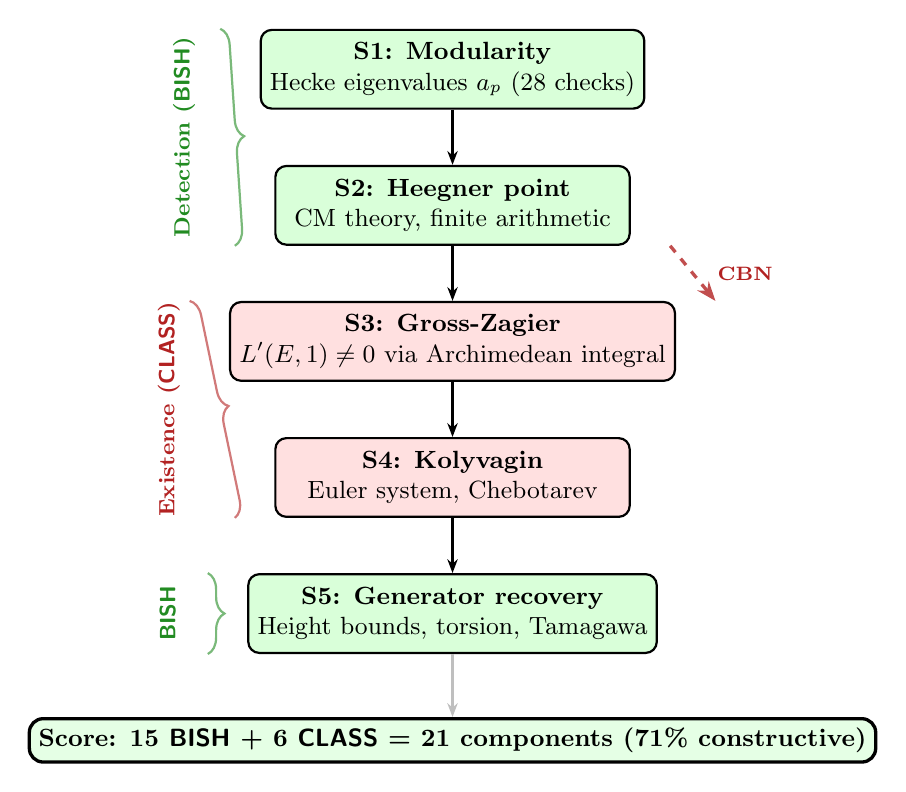
\begin{tikzpicture}[
  bstage/.style={draw, rounded corners=4pt, thick,
    minimum width=4.5cm, minimum height=1cm,
    align=center, font=\small},
  node distance=0.7cm
]
  % BISH stages
  \node[bstage, fill=green!15] (s1)
    {\textbf{S1: Modularity}\\Hecke eigenvalues $a_p$ (28 checks)};
  \node[bstage, fill=green!15, below=of s1] (s2)
    {\textbf{S2: Heegner point}\\CM theory, finite arithmetic};

  % CLASS stages
  \node[bstage, fill=red!12, below=of s2] (s3)
    {\textbf{S3: Gross-Zagier}\\$L'(E,1) \neq 0$ via Archimedean integral};
  \node[bstage, fill=red!12, below=of s3] (s4)
    {\textbf{S4: Kolyvagin}\\Euler system, Chebotarev};

  % BISH again
  \node[bstage, fill=green!15, below=of s4] (s5)
    {\textbf{S5: Generator recovery}\\Height bounds, torsion, Tamagawa};

  % Arrows
  \foreach \a/\b in {s1/s2, s2/s3, s3/s4, s4/s5} {
    \draw[arr] (\a) -- (\b);
  }

  % Side labels
  \draw[decorate, decoration={brace, amplitude=6pt},
        thick, bishgreen!60]
    ([xshift=-5mm]s1.north west) -- ([xshift=-5mm]s2.south west)
    node[midway, left=8pt, font=\footnotesize\bfseries,
         text=bishgreen, rotate=90, anchor=south] {Detection (\BISH)};

  \draw[decorate, decoration={brace, amplitude=6pt},
        thick, classred!60]
    ([xshift=-5mm]s3.north west) -- ([xshift=-5mm]s4.south west)
    node[midway, left=8pt, font=\footnotesize\bfseries,
         text=classred, rotate=90, anchor=south] {Existence (\CLASS)};

  \draw[decorate, decoration={brace, amplitude=6pt},
        thick, bishgreen!60]
    ([xshift=-5mm]s5.north west) -- ([xshift=-5mm]s5.south west)
    node[midway, left=8pt, font=\footnotesize\bfseries,
         text=bishgreen, rotate=90, anchor=south] {\BISH};

  % CBN arrow
  \draw[very thick, dashed, classred!80, -{Stealth[length=7pt]}]
    ([xshift=5mm]s2.south east) -- ([xshift=5mm]s3.north east)
    node[midway, right=5pt, font=\scriptsize\bfseries, text=classred]
      {CBN};

  % Score
  \node[draw, very thick, rounded corners=5pt,
        fill=green!10, minimum width=8cm,
        below=0.8cm of s5, font=\small\bfseries] (score)
    {Score: 15 \BISH{} + 6 \CLASS{} = 21 components (71\% constructive)};
  \draw[arr, gray!50] (s5) -- (score);
\end{tikzpicture}
\caption{The BSD Squeeze pipeline for 37a1 (\paperref{95}). \BISH{} core = pure arithmetic (\texttt{native\_decide}, \texttt{linarith}). \CLASS{} shell = analytic/existential (integration over $\mathbb{R}$, Chebotarev density, duality). 796 lines Lean, 58 theorems, 0 \texttt{sorry}.}
\label{fig:bsd-pipeline}
\end{figure}

The six \CLASS{} components, precisely:
\begin{enumerate}[label=\textbf{C\arabic*:}, leftmargin=2cm]
  \item \textbf{Analytic continuation} of $L(E,s)$ via the Mellin transform. The Euler product converges only for $\mathrm{Re}(s) > 3/2$; extending to $s = 1$ requires integration over $\mathbb{R}$.
  \item \textbf{Rankin-Selberg convolution} in the Gross-Zagier formula. The key identity $L'(E,1) = c \cdot \hat{h}(y_K)$ is proved via the Rankin-Selberg integral, an integration against the Petersson inner product on $\mathrm{SL}_2(\mathbb{Z}) \backslash \mathfrak{H}$---integration over the upper half-plane, which passes through $\mathbb{R}$.
  \item \textbf{Archimedean local heights} via the Green's function on $E(\mathbb{C})$. The canonical height $\hat{h}$ decomposes into local heights $\lambda_v$ at each place $v$; at the Archimedean place, $\lambda_\infty$ involves the Weierstrass $\sigma$-function (a transcendental function of $\mathbb{R}$).
  \item \textbf{Kolyvagin's Euler system} with Chebotarev density. Constructing derivative classes $c_\ell$ for Kolyvagin primes $\ell$ requires that primes with prescribed Frobenius exist in sufficient density---an asymptotic statement about prime distribution over $\mathbb{R}$.
  \item \textbf{Cassels pairing symmetry} via Poitou-Tate duality. The nine-term exact sequence assembles local data at all places simultaneously, using a restricted product over infinitely many primes.
  \item \textbf{Poitou-Tate exact sequence} over infinite extensions. The annihilation of $\Sha[p^\infty]$ for all primes $p$ simultaneously requires the profinite topology of Galois groups.
\end{enumerate}

Every one of these passes through $\mathbb{R}$ or through an infinite topological limit. This confirms the Archimedean Obstruction Thesis (Chapter~7): the sole factory of \CLASS{} content is the Archimedean place.


%── 6.3 ───────────────────────────────────────────────────
\section{The Root Number Bifurcation}

\paperref{96} discovers a BSD bifurcation parallel to the palindromic bifurcation in Hodge. A discrete invariant---the \textbf{root number} $w = \pm 1$---controls the CRM cost.

\begin{figure}[htbp]
\centering
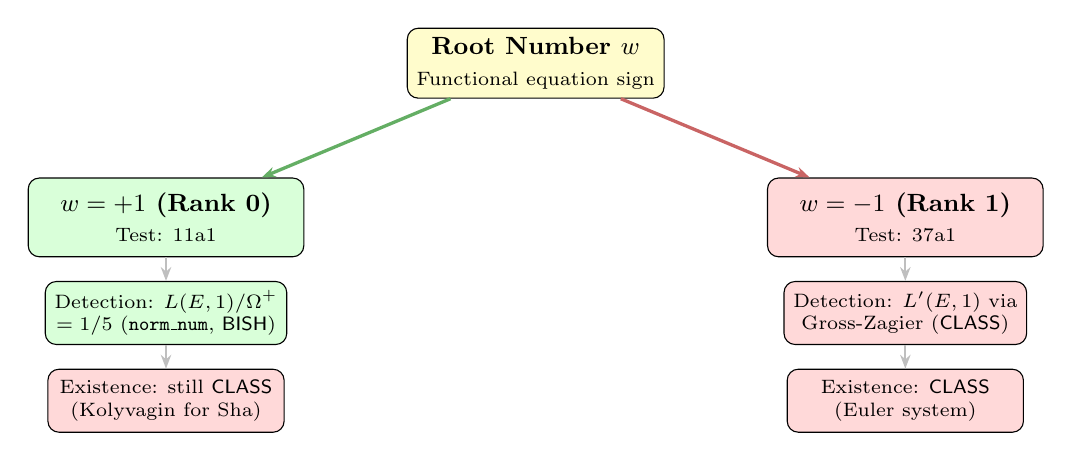
\begin{tikzpicture}[
  node distance=1cm and 1.3cm
]
  % Root
  \node[rootbox, minimum width=3.2cm] (root)
    {\textbf{Root Number $w$}\\{\scriptsize Functional equation sign}};

  % w = +1 branch
  \node[bishbox, minimum width=3.5cm, minimum height=1cm,
        below left=of root] (plus)
    {\textbf{$w = +1$ (Rank 0)}\\{\scriptsize Test: 11a1}};
  \node[bishbox, font=\scriptsize, minimum width=3cm,
        below=0.3cm of plus] (pdet)
    {Detection: $L(E,1)/\Omega^+$\\$= 1/5$ (\texttt{norm\_num}, \BISH)};
  \node[classbox, font=\scriptsize, minimum width=3cm,
        below=0.3cm of pdet] (pex)
    {Existence: still \CLASS\\(Kolyvagin for $\Sha$)};

  % w = -1 branch
  \node[classbox, minimum width=3.5cm, minimum height=1cm,
        below right=of root] (minus)
    {\textbf{$w = -1$ (Rank 1)}\\{\scriptsize Test: 37a1}};
  \node[classbox, font=\scriptsize, minimum width=3cm,
        below=0.3cm of minus] (mdet)
    {Detection: $L'(E,1)$ via\\Gross-Zagier (\CLASS)};
  \node[classbox, font=\scriptsize, minimum width=3cm,
        below=0.3cm of mdet] (mex)
    {Existence: \CLASS\\(Euler system)};

  % Arrows
  \draw[arr, bishgreen!70, very thick] (root) -- (plus);
  \draw[arr, classred!70, very thick] (root) -- (minus);
  \draw[arr, gray!50] (plus) -- (pdet);
  \draw[arr, gray!50] (pdet) -- (pex);
  \draw[arr, gray!50] (minus) -- (mdet);
  \draw[arr, gray!50] (mdet) -- (mex);
\end{tikzpicture}
\caption{Root number bifurcation (\paperref{96}). For $w=+1$, BSD detection is \BISH{} ($L(E,1)/\Omega^+$ computable). For $w=-1$, detection requires Gross-Zagier (\CLASS). Score: 10 \BISH{} + 3 \CLASS{} = 77\%.}
\label{fig:root-number}
\end{figure}


%── 6.4 ───────────────────────────────────────────────────
\section{Why BSD Doesn't Bifurcate Like Hodge}

\begin{analogybox}[Why BSD Is Stuck: The Highway vs.\ the Lane]
The Hodge campaign found a beautiful bifurcation: a codimension-1 locus in a 9-dimensional parameter space where the cost drops from \CLASS{} to \BISH. This works because the parameter space is large enough---like a multi-lane highway with room to change lanes.

Elliptic curves live on the $j$-line: a \emph{one-dimensional} space. There are no lanes to change into. The root number ($\pm 1$) is discrete, not continuous---you're either on one road or the other. And on both roads, the Archimedean $L$-function is unavoidable.

This is the ``null finding'' of \paperref{97}: BSD cannot bifurcate like Hodge because its parameter space is too small.
\end{analogybox}

\paperref{97} systematically explored whether the BSD landscape admits a richer bifurcation and found a definitive negative. Three directions were investigated:

\begin{enumerate}
  \item \textbf{2-Descent Excision.} 2-descent computes the rank constructively (\BISH), but proving Sha finite requires Kolyvagin (\CLASS). Rank and Sha decouple sharply.
  \item \textbf{$p$-Adic Gross-Zagier Bypass.} Coleman's $p$-adic integration is \BISH, but comparison to the Archimedean $L$-function reintroduces $\Omega_+(E)$---circular.
  \item \textbf{Parameter-Space Bifurcation.} This is the structural explanation.
\end{enumerate}

\begin{figure}[htbp]
\centering
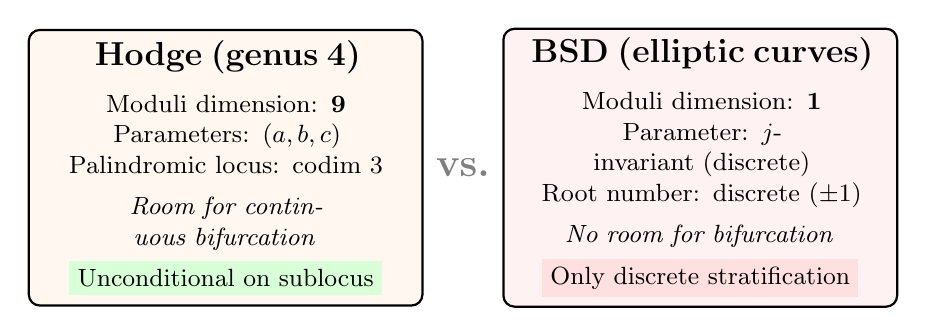
\begin{tikzpicture}[
  cbox/.style={draw, rounded corners=4pt, thick,
    minimum width=5cm, minimum height=3.5cm,
    align=center, font=\small, text width=4.5cm}
]
  % Hodge
  \node[cbox, fill=orange!6] (hodge) {
    \textbf{\large Hodge (genus 4)}\\[6pt]
    Moduli dimension: \textbf{9}\\
    Parameters: $(a, b, c)$\\
    Palindromic locus: codim 3\\[4pt]
    \emph{Room for continuous bifurcation}\\[4pt]
    \colorbox{green!15}{Unconditional on sublocus}
  };

  % BSD
  \node[cbox, fill=red!5, right=1cm of hodge] (bsd) {
    \textbf{\large BSD (elliptic curves)}\\[6pt]
    Moduli dimension: \textbf{1}\\
    Parameter: $j$-invariant (discrete)\\
    Root number: discrete ($\pm 1$)\\[4pt]
    \emph{No room for bifurcation}\\[4pt]
    \colorbox{red!12}{Only discrete stratification}
  };

  % vs label
  \node[font=\Large\bfseries, text=gray] at ($(hodge.east)!0.5!(bsd.west)$) {vs.};
\end{tikzpicture}
\caption{Moduli dimension contrast (\paperref{97}). Genus-4 Jacobians have a 9-dimensional moduli space with room for continuous bifurcation. Elliptic curves are isolated points on the 1-dimensional $j$-line---no room for the palindromic/generic split to emerge.}
\label{fig:moduli-contrast}
\end{figure}

\begin{thesisbox}[Rank/Sha Decoupling Theorem (P97)]
Rank verification is \BISH. Sha finiteness is irreducibly \CLASS. These cannot be bridged. The 71\% \BISH{} figure for BSD will not improve to 90\%.
\end{thesisbox}


%── 6.10 ──────────────────────────────────────────────────
\section{What 71\% Constructive Means}

The BSD Squeeze extracts 71\% \BISH{} content, compared to the Hodge Squeeze's 90\%. This gap is not noise---it reflects a genuine structural difference:

\begin{itemize}
  \item \textbf{Hodge:} The detection problem (``is this class of type $(p,p)$?'') is almost entirely algebraic. Trace vanishing $\tau_+ = 0$ is verified by \texttt{ring} in $\mathbb{Z}[a,b,c]$. The only irreducible \CLASS{} node is the cycle class map (comparing de Rham to Betti cohomology).

  \item \textbf{BSD:} The detection problem (``does $L(E,s)$ vanish at $s=1$?'') involves an $L$-function defined by integration over $\mathbb{R}$. The Gross-Zagier formula, the Petersson norm, the analytic continuation, and the Euler system all pass through the Archimedean place. More of the proof is \emph{inherently analytic}.
\end{itemize}

The 29\% \CLASS{} content (Gross-Zagier + Kolyvagin + Chebotarev + Cassels + Poitou-Tate) is irreducible for rank~1. Every known path to BSD for rank-1 curves passes through the Archimedean $L$-function. There is no known algebraic substitute.

\begin{analogybox}[Analogy: two houses, one power grid]
Both the Hodge house and the BSD house draw power from the same plant ($\mathbb{R}$). But the Hodge house has most appliances running on solar (algebraic, \BISH). Only the front porch light (cycle class map) needs the grid (\CLASS). The BSD house has the heating system (\CLASS---the $L$-function) wired into the grid. You can insulate but you cannot disconnect.
\end{analogybox}


%══════════════════════════════════════════════════════════
% CHAPTER 7
%══════════════════════════════════════════════════════════
\chapter{The Motivic Architecture---Why the Pattern Holds}

\begin{analogybox}[Chapter Preview: The Grand Explanation]
The previous chapters documented a pattern: detection is cheap (\BISH), existence is expensive (\CLASS), and the cost always traces back to $\mathbb{R}$. But \emph{why}?

This chapter answers the question. The key is Grothendieck's theory of \textbf{motives}---a universal algebraic object that encodes all the information about a geometric shape. The motive itself is always free (\BISH). But to \emph{read} the motive, you need a ``lens'' (realization functor). Some lenses are cheap (stay in algebra), others are expensive (pass through $\mathbb{R}$). The cost of a mathematical domain is determined by which lens it uses.

This is not a metaphor. It is a precise, testable prediction: any mathematical theorem whose proof passes through an Archimedean realization (Betti cohomology, Hodge decomposition, $L^2$ spectral theory) will cost \CLASS. Any theorem that stays within algebraic/\mbox{$p$-adic} realizations will be \BISH. All 98 papers of the program confirm this prediction.
\end{analogybox}

\paperref{98} is the grand capstone of the program. It explains \textbf{why} six domains of mathematics have systematically different logical signatures, and how Grothendieck's theory of motives provides the structural explanation.


%── 7.1 ───────────────────────────────────────────────────
\section{The Motive as Universal Certificate}

A \textbf{motive} is the algebraic ``DNA'' of a variety. It captures all cohomological information---Betti numbers, Hodge structure, Galois representation, $L$-function---in a single algebraic object.

The crucial fact: \textbf{the motive itself is always \BISH.} It is a purely algebraic construction. A \textbf{correspondence} between two varieties $X$ and $Y$ is an algebraic cycle living on the product $X \times Y$---think of it as a ``polynomial relation'' between $X$ and $Y$, specified by a finite set of polynomial equations in the combined coordinates. Motives are built from these correspondences using finitary operations (composition, direct sum, tensor product). No topology, no analysis, no $\mathbb{R}$.

But to \emph{extract information} from a motive, you must pass it through a \textbf{realization functor}---a machine that reads the algebraic DNA and produces concrete mathematical data. Each realization functor has a definite CRM cost, and the cost depends on whether the functor passes through the Archimedean place.

\begin{analogybox}[Analogy: Blueprint and Lenses]
The motive is a master blueprint. The blueprint itself is free to copy and examine (\BISH). But to read specific information from it, you need a lens (realization functor). Some lenses are ordinary visible-light lenses (algebraic realizations)---they cost nothing extra. Others are UV lenses (Archimedean realizations)---they require special equipment (\CLASS). The blueprint doesn't change. Only the cost of reading it changes.
\end{analogybox}


%── 7.2 ───────────────────────────────────────────────────
\section{Realization Functors and Their Costs}

The motive contains \emph{all} the information about a variety, but in an abstract algebraic form. To extract concrete data---numbers, matrices, spaces---you must ``realize'' the motive through a specific lens. There are six main lenses, each producing a different type of mathematical object:

\begin{analogybox}[Six Ways to Read the Same DNA]
Think of the motive as the DNA of a geometric shape. Each realization functor is a different laboratory test:
\begin{itemize}
  \item \textbf{de Rham} (algebraic differential forms): Like reading the DNA sequence directly. Pure algebra. Cost: \BISH.
  \item \textbf{\'Etale} ($\ell$-adic Galois representations): Like observing how the DNA responds to specific enzymes (Frobenius symmetries). Finite-field arithmetic. Cost: \BISH.
  \item \textbf{Crystalline} (Witt vector cohomology): Like freeze-drying the DNA and examining the crystal structure. $p$-adic linear algebra. Cost: \BISH.
  \item \textbf{Betti} (singular cohomology): Like dissolving the DNA in water and measuring the topological shape of the resulting protein. Requires integrating over $\mathbb{R}$. Cost: \CLASS.
  \item \textbf{Hodge} ($(p,q)$-decomposition): Like splitting the dissolved protein with a spectroscope. Requires solving elliptic PDEs over $\mathbb{C}$. Cost: \CLASS.
  \item \textbf{Automorphic} ($L^2$ spectral theory): Like analyzing the protein's vibration modes. Requires spectral decomposition on infinite-dimensional Hilbert spaces. Cost: \CLASS.
\end{itemize}
The pattern is sharp: the first three tests stay within algebra or $p$-adic arithmetic. The last three pass through $\mathbb{R}$ (or $\mathbb{C} = \mathbb{R}[i]$). \textbf{Passing through $\mathbb{R}$ is the sole cause of \CLASS{} cost.}
\end{analogybox}

A \textbf{comparison isomorphism} is a theorem that says two different realizations give ``the same'' answer---for example, de Rham-Betti comparison says that algebraic differential forms and topological cycles produce isomorphic cohomology groups. These comparison theorems have definite CRM costs: if both realizations are algebraic, the comparison is \BISH. If one passes through $\mathbb{R}$, the comparison costs \CLASS.

\begin{figure}[htbp]
\centering
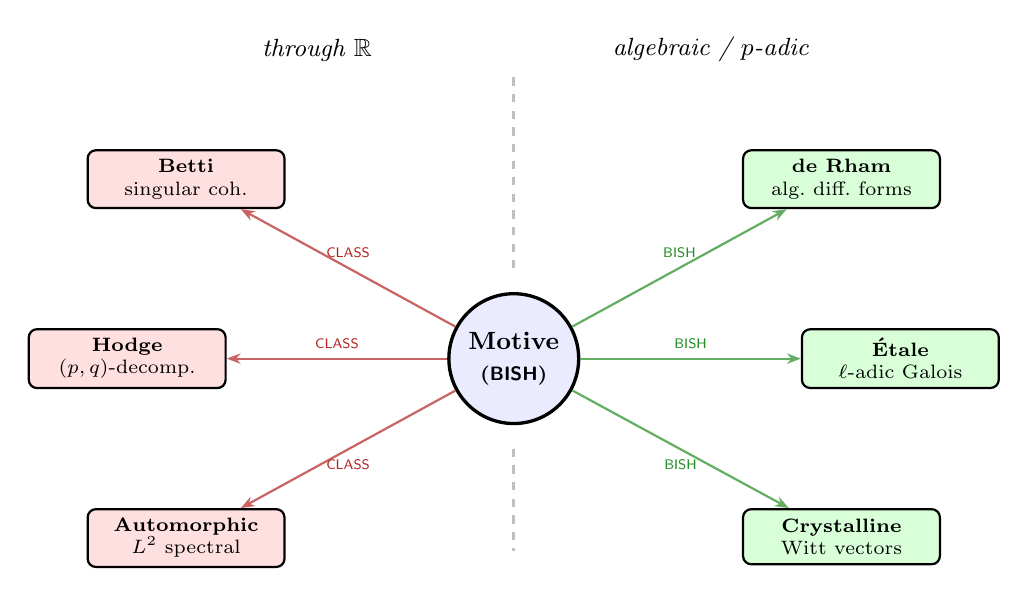
\begin{tikzpicture}[
  rfbox/.style={draw, rounded corners=3pt, thick,
    minimum width=2.5cm, minimum height=0.7cm,
    align=center, font=\scriptsize},
  node distance=0.5cm
]
  % Central motive
  \node[draw, very thick, circle, fill=blue!8,
        minimum size=1.6cm, font=\small\bfseries, align=center] (M) {Motive\\{\scriptsize(\BISH)}};

  % BISH realizations (right)
  \node[rfbox, fill=green!15, above right=1.3cm and 2.3cm of M] (dr)
    {\textbf{de Rham}\\alg.\ diff.\ forms};
  \node[rfbox, fill=green!15, right=2.8cm of M] (et)
    {\textbf{\'Etale}\\$\ell$-adic Galois};
  \node[rfbox, fill=green!15, below right=1.3cm and 2.3cm of M] (cr)
    {\textbf{Crystalline}\\Witt vectors};

  % CLASS realizations (left)
  \node[rfbox, fill=red!12, above left=1.3cm and 2.3cm of M] (be)
    {\textbf{Betti}\\singular coh.};
  \node[rfbox, fill=red!12, left=2.8cm of M] (ho)
    {\textbf{Hodge}\\$(p,q)$-decomp.};
  \node[rfbox, fill=red!12, below left=1.3cm and 2.3cm of M] (au)
    {\textbf{Automorphic}\\$L^2$ spectral};

  % Arrows
  \draw[arr, bishgreen!70, thick] (M) -- (dr)
    node[midway, above, font=\tiny, text=bishgreen] {\BISH};
  \draw[arr, bishgreen!70, thick] (M) -- (et)
    node[midway, above, font=\tiny, text=bishgreen] {\BISH};
  \draw[arr, bishgreen!70, thick] (M) -- (cr)
    node[midway, below, font=\tiny, text=bishgreen] {\BISH};

  \draw[arr, classred!70, thick] (M) -- (be)
    node[midway, above, font=\tiny, text=classred] {\CLASS};
  \draw[arr, classred!70, thick] (M) -- (ho)
    node[midway, above, font=\tiny, text=classred] {\CLASS};
  \draw[arr, classred!70, thick] (M) -- (au)
    node[midway, below, font=\tiny, text=classred] {\CLASS};

  % Labels
  \node[above=2.8cm of M, font=\small\itshape, xshift=-2.5cm]
    {through $\mathbb{R}$};
  \node[above=2.8cm of M, font=\small\itshape, xshift=2.5cm]
    {algebraic / $p$-adic};

  % Divider
  \draw[very thick, dashed, gray!50] (M.north) ++(0,0.3) -- ++(0,2.5);
  \draw[very thick, dashed, gray!50] (M.south) ++(0,-0.3) -- ++(0,-1.3);
\end{tikzpicture}
\caption{Realization functors and CRM costs (\paperref{98}). Realizations through $\mathbb{R}$ (left) cost \CLASS. Algebraic/$p$-adic realizations (right) are \BISH. The motive itself is \BISH.}
\label{fig:realization-functors}
\end{figure}


%── 7.3 ───────────────────────────────────────────────────
\section{The Archimedean Obstruction Thesis}

\paperref{98} formalizes the central finding as a single principle:

\begin{thesisbox}[The Archimedean Obstruction Thesis]
Every comparison isomorphism between realizations that passes through the Archimedean place costs \CLASS. Every comparison that stays within algebraic/$p$-adic realizations is \BISH. The Archimedean place is the sole factory of \CLASS{} content.
\end{thesisbox}

\paragraph{Is this just a tautology?} One might worry that ``the classical content comes from $\mathbb{R}$'' merely restates ``analysis requires analysis.'' The explanatory power lies in the thesis's \emph{falsifiable structural predictions}: if the Archimedean place is the sole source, then removing it entirely must yield a strictly \BISH{} proof architecture---even for the deepest theorems. This is confirmed by the function field Langlands correspondence (\paperref{69}), where the ad\`ele ring has no Archimedean factor and the entire proof is \BISH. The thesis also predicts (see Appendix~\ref{app:frontiers}) that the $p$-adic Langlands correspondence, motivic Iwasawa theory, and local $\GL_n$ Langlands should all be constructive. These predictions are untested and could fail. If they hold, the thesis explains; if they fail, we discover new obstructions. Either way, it generates research.

This principle explains all 98 papers:

\begin{itemize}
  \item \textbf{Physics} (\paperref{1--44}): The spectral theorem requires \LPO{} because it operates on $\mathbb{R}$. Lattice physics (no $\mathbb{R}$) is \BISH.
  \item \textbf{Function field Langlands} (\paperref{69}): Over $\mathbb{F}_q(t)$, the adele ring has no Archimedean factor. Entire correspondence is \BISH.
  \item \textbf{Hodge campaign} (\paperref{84--93}): Hodge realization passes through $\mathbb{R}$. Detection at the algebraic level (de Rham) is \BISH. Existence (comparison to Betti) is \CLASS.
  \item \textbf{BSD} (\paperref{95--97}): $L$-function passes through $\mathbb{R}$ (Mellin transform). Hecke arithmetic (\'etale) is \BISH. Analytic continuation and Gross-Zagier are \CLASS.
  \item \textbf{FLT} (\paperref{68}): Taylor-Wiles patching replaced the Petersson inner product (integration over $\mathbb{R}$: \CLASS) with an algebraic inverse limit. Logical excision of the Archimedean bottleneck.
\end{itemize}


%── 7.4 ───────────────────────────────────────────────────
\section{Three Calibration Theorems}

\paperref{98}, \S\S6--8 verifies the Archimedean Obstruction Thesis against three calibration points spanning different domains. Each calibration is a precise, falsifiable prediction:

\paragraph{Calibration I: Hodge detection $\longleftrightarrow$ WLPO (\paperref{86--90}).}
The Hodge realization passes through $\mathbb{R}$. Generic detection costs WLPO (real-number equality test for period matrix entries). With CM metadata---which provides an algebraic shortcut past $\mathbb{R}$---the cost drops to \BISH. The palindromic locus of the universal family $C_{a,b,c}$ provides this shortcut (Kani-Rosen splitting, \paperref{86}). The generic locus does not. The Archimedean Obstruction Thesis predicts exactly this: the shortcut exists if and only if an algebraic substitute for the Archimedean comparison is available.

\paragraph{Calibration II: Taylor-Wiles patching $\longleftrightarrow$ WKL (\paperref{68--71}).}
Wiles's 1993 attempt at FLT used the \textbf{Petersson inner product}---integration over a non-compact modular surface, involving $\mathbb{R}$---costing \CLASS. The Taylor--Wiles patch (1995) replaced this analytic ingredient with an \textbf{algebraic inverse limit} over finite level structures. In CRM terms: the patch excised the Archimedean bottleneck. The replacement principle is \textbf{WKL} (\textbf{Weak K\"onig's Lemma}): every infinite binary tree has an infinite path. In classical reverse mathematics, WKL is strictly weaker than arithmetic comprehension and captures exactly the compactness arguments of analysis. In CRM terms, WKL lies between \BISH{} and \LPO{} (it is implied by \LPO{} but does not imply it). The TW prime search is \BISH{} (effective Chebotarev bounds: Lagarias--Montgomery--Odlyzko 1979, Ahn--Kwon 2019), and Brochard's finite-level criterion (2017) eliminates the Fan Theorem. But the inverse limit assembling $R_\infty$ from compatible finite approximations is irreducibly \WKL{} (\paperref{98}, Calibration Theorem~II; confirmed by \paperref{99}). The result: $\mathrm{CRM}(\mathrm{FLT}) = \WKL$. This is a historical case of de-omniscientizing descent: the mathematical community found a cheaper proof by (inadvertently) removing the Archimedean computation, but the non-Archimedean compactness in patching is irreducible.

\paragraph{Calibration III: BSD rank/Sha decoupling (\paperref{95--97}).}
Rank verification uses \'etale/algebraic methods (\BISH). Sha finiteness requires the Archimedean $L$-function (\CLASS). No bifurcation is possible because the elliptic curve moduli has dimension~1 (no room for a continuous family). The Archimedean $\Gamma$-factor, the period integral $\Omega_+(E)$, and the Mellin transform defining $L(E,s)$ all pass through $\mathbb{R}$.

\begin{keyrefbox}
  Three domains (Hodge theory, Galois representations, BSD arithmetic), three different proof technologies, one uniform prediction: the cost boundary falls exactly where the Archimedean place enters. The thesis is not fitted to the data---it was formulated (\paperref{70}, 2025) before the Squeeze applications (\paperref{80--96}, 2026) that tested it.
\end{keyrefbox}


%── 7.5 ───────────────────────────────────────────────────
\section{The Six-Domain Signature Map}

Every branch of mathematics has a characteristic ``CRM signature''---a fingerprint that reveals which realization functor it primarily uses. The signature is not assigned by fiat; it emerges automatically from the Archimedean Obstruction Thesis.

\begin{analogybox}[Analogy: Neighborhoods and the Power Grid]
Think of mathematics as a city with six neighborhoods. Each neighborhood draws its power from different sources. Algebraic Geometry and Representation Theory have solar panels (algebraic, self-contained, \BISH). Number Theory has solar plus a small diesel generator (\BISH{} + \MP). Physics has solar plus a medium generator (\BISH{} + \LPO). Topology and Harmonic Analysis draw all their power from the municipal grid ($\mathbb{R}$, i.e., \CLASS).

The Archimedean Obstruction Thesis explains the grid: the sole municipal power plant is $\mathbb{R}$. Neighborhoods that plug into it pay the \CLASS{} tariff. Those with independent power don't.
\end{analogybox}

\begin{figure}[htbp]
\centering
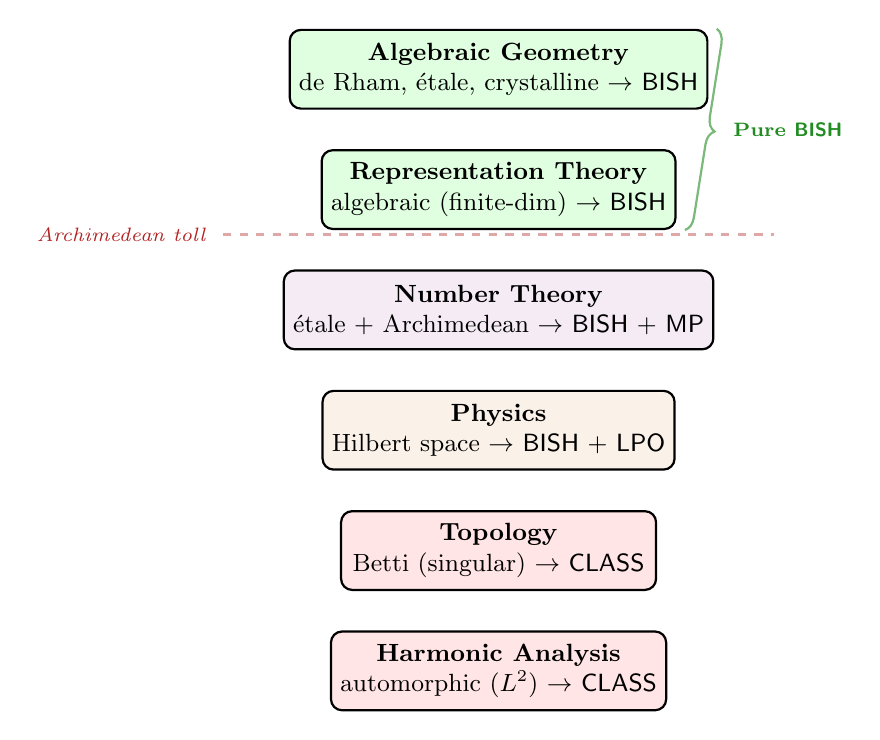
\begin{tikzpicture}[
  dbox/.style={draw, rounded corners=4pt, thick,
    minimum width=4cm, minimum height=1cm,
    align=center, font=\small},
  node distance=0.5cm
]
  \node[dbox, fill=green!12] (ag)
    {\textbf{Algebraic Geometry}\\de Rham, \'etale, crystalline $\to$ \BISH};
  \node[dbox, fill=green!12, below=of ag] (rt)
    {\textbf{Representation Theory}\\algebraic (finite-dim) $\to$ \BISH};
  \node[dbox, fill=mppurple!8, below=of rt] (nt)
    {\textbf{Number Theory}\\\'etale + Archimedean $\to$ \BISH{} + \MP};
  \node[dbox, fill=lpoamber!10, below=of nt] (ph)
    {\textbf{Physics}\\Hilbert space $\to$ \BISH{} + \LPO};
  \node[dbox, fill=red!10, below=of ph] (tp)
    {\textbf{Topology}\\Betti (singular) $\to$ \CLASS};
  \node[dbox, fill=red!10, below=of tp] (ha)
    {\textbf{Harmonic Analysis}\\automorphic ($L^2$) $\to$ \CLASS};

  % Divider line
  \draw[very thick, dashed, classred!40]
    (-3.5, -2.1) -- (3.5, -2.1);
  \node[font=\scriptsize\itshape, text=classred, anchor=east] at (-3.6, -2.1)
    {Archimedean toll};

  % Brace for BISH sector
  \draw[decorate, decoration={brace, amplitude=5pt},
        thick, bishgreen!60]
    ([xshift=3pt]ag.north east) -- ([xshift=3pt]rt.south east)
    node[midway, right=8pt, font=\scriptsize\bfseries, text=bishgreen] {Pure \BISH};
\end{tikzpicture}
\caption{Six-domain signature map (\paperref{98}). Each domain's CRM signature reflects which realization it uses. Domains below the Archimedean toll line pass through $\mathbb{R}$ and pay the cost.}
\label{fig:six-domain}
\end{figure}


%── 7.6 ───────────────────────────────────────────────────
\section{The Detection/Existence Table---Now Explained}

\begin{analogybox}[Detection vs.\ Existence: The Recipe Analogy]
\textbf{Detection} is like having a recipe and checking whether a dish matches it. You compare ingredients, temperatures, cooking times---all verifiable by inspection. Cost: cheap (\BISH).

\textbf{Existence} is like being told ``a restaurant in this city serves this dish'' without being told \emph{which} restaurant. You must search the entire city. Cost: expensive (\CLASS).

Now we can explain \emph{why} this is universal: detection uses algebraic realizations (de Rham, \'etale)---reading the motive under visible light. Existence uses topological/analytic realizations (Betti, Hodge, automorphic)---reading it under UV light. The motive is the same; the cost depends on the lens.
\end{analogybox}

The universal pattern across the program---detection is \BISH, existence is \CLASS---is now explained by the motivic architecture:

\begin{table}[htbp]
\centering\small
\caption{Detection/existence bifurcation across all Squeeze applications. Detection uses algebraic realizations (\BISH). Existence uses analytic realizations (\CLASS).}
\label{tab:detection-existence}
\renewcommand{\arraystretch}{1.3}
\begin{tabular}{@{}l p{4cm} p{4cm}@{}}
\toprule
\textbf{Domain} & \textbf{Detection (\BISH)} & \textbf{Existence (\CLASS)} \\
\midrule
\rowcolor{green!4}
Hodge (\paperref{84--89}) & $\tau_+ = 0$ (trace vanishing, \texttt{ring} in $\mathbb{Z}[a,b,c]$) & Algebraic cycle (VHC or Kani-Rosen) \\
\rowcolor{green!4}
CY3 (\paperref{94}) & $\delta(z) \neq 0$ (source term, \texttt{norm\_num}) & Abel-Jacobi map, Baire category \\
\rowcolor{green!4}
BSD (\paperref{95--96}) & $a_p$ computation, $\hat{h}(y_K) > 0$ (\texttt{native\_decide}, \texttt{linarith}) & Kolyvagin, Chebotarev, Poitou-Tate \\
\rowcolor{green!4}
Langlands (\paperref{78}) & Character-trace matching (\texttt{decide} over $\mathbb{Z}$) & Harris-Taylor existence (global Shimura) \\
\rowcolor{green!4}
Picard (\paperref{83}) & Flat section dim = 1 (\texttt{ring} over $\mathbb{Q}(t)$) & Topological monodromy (Ehresmann, Deligne) \\
\bottomrule
\end{tabular}
\end{table}

\begin{thesisbox}[The 80\% Rule]
Across 15+ Squeeze applications, median 80+\% of formal content is \BISH. Classical content is concentrated in a small number of CBN nodes. This is not because mathematics is ``mostly easy''---it is because the bulk of any proof is algebraic machinery (detection), while the irreducible classical content (existence) is confined to a few topological existence assertions.
\end{thesisbox}


%══════════════════════════════════════════════════════════
% CHAPTER 8
%══════════════════════════════════════════════════════════
\chapter{Applying the Framework}

The CRM framework and Squeeze protocol are not limited to the specific theorems audited in Papers~1--98. They constitute a general methodology applicable to any mathematical proof. This chapter gives practical guidance for using the framework, with examples for several audiences.


%── 8.1 ───────────────────────────────────────────────────
\section{How to Do a CRM Audit: Five Steps}

Any theorem with a proof can be audited for logical cost. The procedure:

\begin{enumerate}
  \item \textbf{Identify the theorem.} Write the statement precisely. What does it claim exists? What equality or inequality does it assert? Does the statement itself require an oracle (e.g., ``for all $x \in \mathbb{R}$, either $x > 0$ or $x \leq 0$'')?

  \item \textbf{Trace the proof steps.} For each step, ask: does this step produce a \emph{witness} (an explicit object: a number, a function, a bound), or does it assert \emph{existence} (something exists, but we don't construct it)?

  \item \textbf{Classify each step.}
  \begin{itemize}
    \item \emph{Witness produced, finite computation:} \BISH.
    \item \emph{Equality test for a real number:} WLPO.
    \item \emph{Search over an infinite set for something that might not exist:} LPO.
    \item \emph{Existence by contradiction, compactness, or Zorn's lemma:} \CLASS.
    \item \emph{Unbounded search that cannot fail:} MP.
  \end{itemize}

  \item \textbf{Find the CBN.} The Classical Boundary Node is where the proof transitions from \BISH{} to \CLASS. This is typically a single step: an appeal to analytic continuation, a limit existence theorem, a compactness argument, or a density result.

  \item \textbf{Measure the conservation gap.} Compare the logical cost of the \emph{statement} to the logical cost of the \emph{proof}. If the statement is \BISH{} but the proof is \CLASS, the gap is nonzero---and a simpler proof may exist.
\end{enumerate}

\begin{figure}[htbp]
\centering
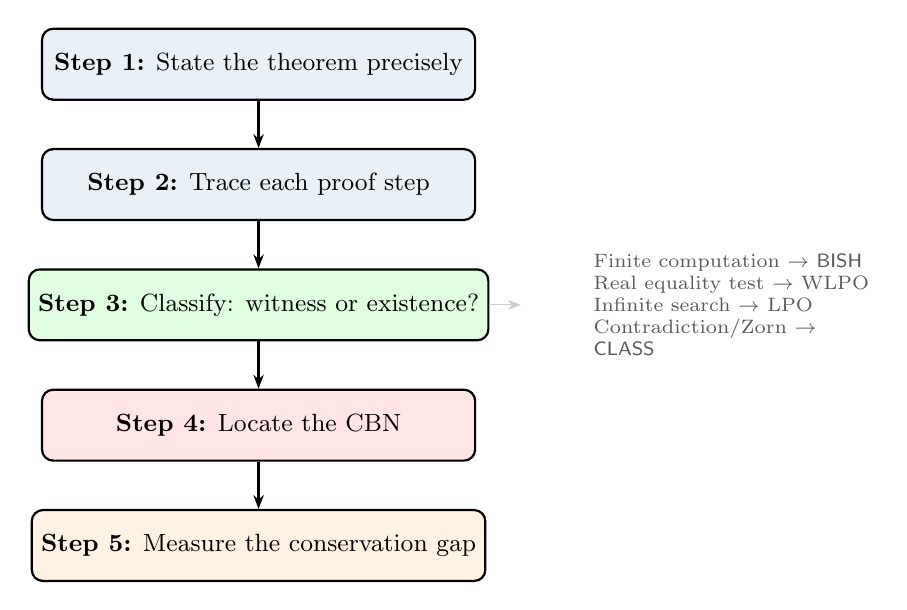
\begin{tikzpicture}[
  auditbox/.style={draw, rounded corners=4pt, thick,
    minimum width=5.5cm, minimum height=0.9cm,
    align=center, font=\small},
  node distance=0.6cm
]
  \node[auditbox, fill=bridgeblue!12] (s1) {\textbf{Step 1:} State the theorem precisely};
  \node[auditbox, fill=bridgeblue!12, below=of s1] (s2) {\textbf{Step 2:} Trace each proof step};
  \node[auditbox, fill=green!12, below=of s2] (s3) {\textbf{Step 3:} Classify: witness or existence?};
  \node[auditbox, fill=red!10, below=of s3] (s4) {\textbf{Step 4:} Locate the CBN};
  \node[auditbox, fill=orange!10, below=of s4] (s5) {\textbf{Step 5:} Measure the conservation gap};

  \foreach \a/\b in {s1/s2, s2/s3, s3/s4, s4/s5} {
    \draw[arr] (\a) -- (\b);
  }

  \node[right=1.2cm of s3, font=\scriptsize, text width=3.5cm, align=left,
        text=gray!70!black] {%
    Finite computation $\to$ \BISH\\
    Real equality test $\to$ WLPO\\
    Infinite search $\to$ LPO\\
    Contradiction/Zorn $\to$ \CLASS};
  \draw[gray!40, -Stealth] (s3.east) -- ++(0.4,0);
\end{tikzpicture}
\caption{The five-step CRM audit procedure. Steps 1--2 are mathematical analysis. Steps 3--5 are CRM classification.}
\label{fig:audit-steps}
\end{figure}


%── 8.2 ───────────────────────────────────────────────────
\section{Cross-Domain Applications}

\subsection*{For Product Managers: Technical Debt as Conservation Gap}

The conservation gap has a direct analogue in software engineering: \textbf{technical debt}. A codebase where the implementation (proof) is more complex than the specification (statement) has a conservation gap. The CRM audit procedure maps directly:

\begin{itemize}
  \item \emph{Core logic} (business rules, algorithms) $=$ \BISH. These are deterministic, testable, and efficient. \textbf{Leave them alone.}
  \item \emph{Infrastructure scaffolding} (caching layers, indeterminate-timeout operations, legacy adapters) $=$ possibly higher-cost. Audit for simplification.
  \item \emph{Conservation gap} $=$ the scaffolding that exists because of historical accident, not structural necessity. Reducing this gap is the highest-leverage refactoring.
\end{itemize}

The CRMLint Squeeze protocol has a software analogue: \textbf{dependency analysis}. Trace each module's dependencies. Flag the ones that introduce the most complexity. Ask: is this dependency \emph{structural} (the feature requires it) or \emph{scaffolding} (a simpler implementation exists)?

\subsection*{For Physicists: The Measurement Problem Dissolved}

\paperref{44} showed that the ``measurement problem'' in quantum mechanics---the apparent collapse of the wave function---is not a single problem but three logically distinct interpretations with different CRM signatures:

\begin{itemize}
  \item \textbf{Copenhagen:} \BISH{} + LPO. The collapse postulate is an oracle (LPO: ``does the detector click?'') applied to the quantum state.
  \item \textbf{Many-Worlds:} \BISH{} + LPO. No collapse, but decoherence requires the spectral theorem (LPO) to split Hilbert space into branches.
  \item \textbf{Bohmian:} \BISH{} + MP. The guiding equation $m\dot{x} = \hbar\,\mathrm{Im}(\nabla\psi/\psi)$ is deterministic, but computing the particle's trajectory requires iterating the velocity field to convergence. Since the velocity depends on the global wave function (which may have arbitrarily fine structure), you know the iteration terminates (the trajectory exists by Picard-Lindel\"of) but you don't know when to within any fixed bound---this is exactly Markov's Principle.
\end{itemize}

All three are logically distinct but empirically equivalent (they agree on all measurable predictions at \BISH{} + LPO). CRM dissolves the metaphysical debate: the three interpretations are three ways of \emph{distributing} the same logical cost across the formalism.

\subsection*{For Graduate Students: Reading Proofs with CRM Eyes}

Every proof you read can be audited informally:
\begin{itemize}
  \item Every ``there exists'' without an explicit construction $=$ \CLASS.
  \item Every appeal to compactness, Zorn's lemma, or the axiom of choice $=$ \CLASS.
  \item Every limit whose convergence rate is unknown $=$ at least MP.
  \item Every spectral decomposition over $\mathbb{R}$ $=$ LPO (spectral theorem).
  \item Everything else $=$ \BISH.
\end{itemize}
The CRM hierarchy gives you a new annotation layer for proofs. When you encounter a difficult proof, ask: is the difficulty \emph{structural} (the theorem genuinely needs this logical power) or \emph{scaffolding} (the author chose a classical shortcut)?

\subsection*{For AI/ML Practitioners: Scaffolding vs.\ Structure in Model Architectures}

The CRM finding that proof complexity $\neq$ logical cost has a direct analogue in neural network design. Complex architectures (many layers, attention heads, skip connections) may be \emph{scaffolding}: the underlying function learned is simpler than the architecture used to learn it. Knowledge distillation, pruning, and neural architecture search are informal versions of the Squeeze protocol: compress the model, test whether the compressed version achieves the same performance, and identify which components are structural vs.\ scaffolding.

A deeper connection: CRM distinguishes \emph{logical cost} (what principles a result needs) from \emph{proof complexity} (how many steps the proof takes). Similarly, in ML, \emph{sample complexity} (how much data a function needs) differs from \emph{model complexity} (how many parameters the architecture has). A 10-billion-parameter model that implements a function learnable by a 1-million-parameter model has a ``conservation gap''---and that gap is the target for distillation. CRM-trained AI could learn to predict which mathematical proofs have analogous gaps, guiding automated simplification.


%── 8.3 ───────────────────────────────────────────────────
\section{CRMLint at Scale: The Mathlib Vision}

The ultimate application of the Squeeze protocol is to \textbf{audit all of Mathlib}---the 150,000+ declaration library of formally verified mathematics in Lean~4.

Running CRMLint on Mathlib would produce a \textbf{proof technique atlas}: for every declaration, the CRM classification and conservation gap. This atlas would reveal:
\begin{itemize}
  \item Which proof techniques are scaffolding (used everywhere, never structural).
  \item Where conservation gaps predict simpler proofs exist.
  \item Which domains of mathematics are ``logically cheap'' (mostly \BISH) and which are ``logically expensive'' (depend on \CLASS{} principles).
\end{itemize}

The 98-paper CRM program is the \textbf{calibration dataset} for this larger project. Its 14 Lean bundles provide ground truth: we know the correct CRM classification for each theorem, verified by human audit. Any automated tool must reproduce these classifications to be trusted.

\begin{thesisbox}[The CRMLint Vision]
CRMLint on Mathlib = \texttt{npm audit} for mathematical proofs. Conservation gaps = technical debt. AI trained on CRM-classified proofs can learn to \emph{predict} where simpler proofs exist and \emph{generate} search targets for proof simplification.
\end{thesisbox}


%══════════════════════════════════════════════════════════
% CHAPTER 9
%══════════════════════════════════════════════════════════
\chapter{Conclusion}


%── 9.1 ───────────────────────────────────────────────────
\section{What the Programme Proved}

The 98-paper CRM program established, with machine-checked proofs:

\begin{enumerate}
  \item \textbf{The physics ceiling is \BISH{} + LPO} (\paperref{29, 35}). Every empirical physical theory calibrated (quantum mechanics, general relativity, QCD, statistical mechanics, scattering theory) fits within this ceiling. LPO enters through the spectral theorem for unbounded self-adjoint operators over $\mathbb{R}$. Fan Theorem and Dependent Choice are dispensable (\paperref{30, 31}).

  \item \textbf{Five great conjectures all exhibit de-omniscientizing descent} (\paperref{45--49}). Full cost: LPO or \CLASS. With algebraic metadata: \BISH{} or \BISH{} + MP. The metadata is always a positive-definite structure from $\mathbb{R}$.

  \item \textbf{DPT axioms are canonical} (\paperref{72--74}). Each is biconditional with decidability in its domain: Standard Conjecture~D $\Leftrightarrow$ morphism decidability; Algebraic Spectrum $\Leftrightarrow$ eigenvalue decidability; Archimedean Polarization $\Leftrightarrow$ cycle-search decidability. No alternative axiom substitutes for any of them.

  \item \textbf{The Squeeze protocol automates CRM discovery} (\paperref{76--96}). Scaffold $\to$ X-Ray $\to$ Excise $\to$ Squeeze. Across 15+ applications, $>$80\% of formal content is \BISH. \CLASS{} content is confined to a small number of CBN nodes: analytic continuation, Euler systems, topological existence assertions.

  \item \textbf{The motivic architecture explains why} (\paperref{98}). Motives are \BISH. Each realization functor has a definite CRM cost. Realizations that pass through $\mathbb{R}$ cost \CLASS. Everything else is \BISH. The Archimedean Obstruction Thesis is a single principle that explains all 98 papers.
\end{enumerate}


%── 9.2 ───────────────────────────────────────────────────
\section{What Remains Open}

\textbf{The conservation conjecture.} Is the \CLASS{} scaffolding in Fargues-Scholze proofs eliminable? DPT and condensed mathematics partition arithmetic into complementary sectors (discrete/\BISH{} vs.\ continuous/\CLASS). The interface between them---five specific questions in \paperref{75}, \S6.5---is open.

\textbf{CRMLint at scale.} What does the full atlas of Mathlib look like? How many declarations have conservation gaps? Can AI exploit these gaps to find simpler proofs?

\textbf{Standard Conjecture D for abelian fourfolds.} Axiom~1 of DPT. Proved for abelian varieties of dimension $\leq 3$ (Lieberman, Tate). Open for dimension~4+.

\textbf{Intermediate axiom sets.} Are there natural logical systems strictly between \BISH{} and LPO? WKL (Weak K\"onig's Lemma) appears in the Taylor-Wiles calibration (\paperref{98}). Is there a natural family of such intermediate systems?


%── 9.3 ───────────────────────────────────────────────────
\section{The Deeper Claim}

CRM is not a restriction of mathematics. It is a sharper lens.

The program did not weaken any theorem. It did not replace any proof. It measured something that was previously invisible: the logical cost of mathematical operations across the domains it surveyed---mathematical physics, arithmetic geometry, representation theory, and selected areas of algebraic geometry. Within these domains, it found consistent structure:

\begin{itemize}
  \item The \textbf{$h = f$ identity}---self-intersection equals conductor on CM abelian fourfolds (\paperref{56--58})---discovered by tracing where equality testing enters.
  \item The \textbf{algebraic-vs-transcendental boundary} (\paperref{69})---discovered by comparing number fields ($\mathbb{R}$) to function fields (no $\mathbb{R}$).
  \item The \textbf{detection/existence bifurcation} (\paperref{84--96})---discovered by separating algebraic computation from topological existence.
  \item The \textbf{palindromic/root-number parallel} (\paperref{86, 96})---discovered by tracing where discrete invariants control CRM cost.
\end{itemize}

None of these were discovered by asking classical questions. They were discovered by asking \textbf{``what does this cost?''}---a question classical mathematics never asks.

\begin{center}
\emph{98 papers. One question. One answer.}\\[4pt]
\textbf{The logical cost of mathematics is the logical cost of $\mathbb{R}$.}
\end{center}


%══════════════════════════════════════════════════════════
% APPENDICES
%══════════════════════════════════════════════════════════
\appendix


%── Appendix A ──────────────────────────────────────────
\chapter{Complete Paper List}

\begingroup
\setlength{\LTleft}{0pt}
\setlength{\LTright}{0pt}
\small
\begin{longtable}{@{}r p{7.5cm} l l@{}}
\toprule
\textbf{No.} & \textbf{Title} & \textbf{Status} & \textbf{DOI suffix} \\
\midrule
\endfirsthead
\toprule
\textbf{No.} & \textbf{Title} & \textbf{Status} & \textbf{DOI suffix} \\
\midrule
\endhead
\bottomrule
\endfoot
  1 & [Withdrawn] & --- & --- \\
  2 & The Bidual Gap and WLPO & Active & 18501689 \\
  3 & [Withdrawn] & --- & --- \\
  4 & Axiom Calibration for Quantum Spectra & Active & 17118223 \\
  5 & Schwarzschild Curvature Verification & Active & 18489703 \\
  6 & Heisenberg Uncertainty (v2) & Active & 18519836 \\
  7 & Physical Bidual Gap, Trace-Class Operators & Active & 18527559 \\
  8 & 1D Ising Model and LPO & Active & 18516813 \\
  9 & Ising Formulation-Invariance & Active & 18517570 \\
 10 & Logical Geography of Mathematical Physics & Active & 18636180 \\
 11 & Entanglement, CHSH, Tsirelson Bound & Active & 18527676 \\
 12 & Constructive History of Mathematical Physics & Active & 18636250 \\
 13 & Event Horizon as Logical Boundary & Active & 18529007 \\
 14 & Quantum Decoherence & Active & 18569068 \\
 15 & Noether Theorem & Active & 18572494 \\
 16 & Born Rule (Technical Note) & Active & 18575377 \\
 17 & Bekenstein-Hawking Formula & Active & 18597306 \\
 18 & Yukawa RG Constructive Stratification & Active & 18626839 \\
 19 & WKB Tunneling and LLPO & Active & 18602596 \\
 20 & Observable-Dependent Logical Cost, 1D Ising & Active & 18603079 \\
 21 & Bell Nonlocality and LLPO & Active & 18603251 \\
 22 & Markov's Principle and Radioactive Decay & Active & 18603503 \\
 23 & Fan Theorem and Optimization & Active & 18604312 \\
 24 & Kochen-Specker Contextuality and LLPO & Active & 18604317 \\
 25 & Choice Axis (CC, DC) and Ergodic Theorems & Active & 18615453 \\
 26 & Bidual Gap Arithmetic Route, WLPO & Active & 18615457 \\
 27 & Bell Angle Optimisation via IVT, LLPO & Active & 18615459 \\
 28 & Newton vs.\ Lagrange vs.\ Hamilton & Active & 18616620 \\
 29 & Fekete's Subadditive Lemma and LPO & Active & 18643617 \\
 30 & Physical Dispensability of the Fan Theorem & Active & 18638394 \\
 31 & Physical Dispensability of Dependent Choice & Active & 18645578 \\
 32 & QED One-Loop: The Landau Pole & Active & 18642598 \\
 33 & QCD One-Loop and Confinement & Active & 18642610 \\
 34 & Scattering Amplitudes Are Constructively Computable & Active & 18642612 \\
 35 & Logical Constitution of Empirical Physics: Metatheorem & Active & 18642616 \\
 36 & Spectral Gap Undecidability: Cubitt $=$ LPO & Active & 18642620 \\
 37 & Undecidability Landscape Is LPO & Active & 18642802 \\
 38 & Wang Tiling and Origin of Physical Undecidability & Active & 18642804 \\
 39 & Beyond LPO: Physical Stratification & Active & 18642806 \\
 40 & Logical Constitution of Physical Reality (Monograph) & Active & 18654773 \\
 41 & AdS/CFT Diagnostic & Active & 18654780 \\
 42 & Cosmological Constant Problem & Active & 18654789 \\
 43 & What the Ceiling Means: Constructive Schools & Active & 18665418 \\
 44 & Measurement Problem Dissolved & Active & 18671162 \\
\midrule
 45 & Weight-Monodromy Conjecture and LPO & Active & 18676170 \\
 46 & Tate Conjecture and LPO & Active & 18682285 \\
 47 & Fontaine-Mazur Conjecture and LPO & Active & 18682788 \\
 48 & BSD Conjecture and LPO & Active & 18683400 \\
 49 & Hodge Conjecture and Constructive Omniscience & Active & 18683802 \\
 50 & Three Axioms for the Motive & Active & 18705837 \\
 51 & Constructive Archimedean Rescue in BSD & Active & 18732168 \\
 52 & Decidability Transfer: Conj~D, Abelian 3-folds & Active & 18732559 \\
 53 & CM Decidability Oracle & Active & 18713089 \\
 54 & Bloch-Kato Calibration & Active & 18732964 \\
 55 & K3 Surfaces, Kuga-Satake, and DPT & Active & 18733731 \\
 56 & Exotic Weil Self-Intersection on CM Abelian 4-folds & Active & 18734021 \\
 57 & Exotic Weil Self-Intersection Across Nine Heegner Fields & Active & 18735172 \\
 58 & Class Number Correction for Exotic Weil Classes & Active & 18734718 \\
 59 & De Rham Decidability and DPT Completeness & Active & 18735931 \\
 60 & [Retired---merged into Paper 59] & --- & --- \\
 61 & Lang's Conjecture as the MP$\to$\BISH{} Gate & Active & 18736959 \\
 62 & [Retired---merged into Paper 63] & --- & --- \\
 63 & The Intermediate Jacobian Obstruction & Active & 18736965 \\
 64 & Uniform $p$-Adic Decidability for Elliptic Curves & Active & 18737090 \\
 65 & Self-Intersection Patterns Beyond Cyclic Cubics & Active & 18743151 \\
 66 & Form-Class Resolution for Non-Cyclic Totally Real Cubics & Active & 18745722 \\
 67 & The Motive Is a Decidability Certificate (Monograph) & Active & 18902506 \\
 68 & The Logical Cost of Fermat's Last Theorem & Active & 18901011 \\
 69 & Function Field Langlands Is \BISH & Active & 18749757 \\
 70 & The Archimedean Principle (Capstone) & Active & 18901192 \\
 71 & Archimedean Principle in Cryptography & Active & 18752015 \\
 72 & The DPT Characterization Theorem & Active & 18765393 \\
 74 & Algebraic Spectrum Is Necessary & Active & 18773827 \\
 75 & Conservation Test: Genestier-Lafforgue LLC & Active & 18773831 \\
\midrule
 76 & CRMLint: Automated CRM Logical Cost Analysis & Active & 18779362 \\
 77 & Explicit Hodge Decompositions for $E^4$ & Active & 18777596 \\
 78 & Explicit Local Langlands, Wildly Ramified & Active & 18789008 \\
 79 & [Unassigned] & --- & --- \\
 80 & Algebraic Gauss-Manin via Griffiths Pole Reduction & Active & 18791985 \\
 81 & Fixed Part Theorem via Tensor Gauss-Manin & Active & 18801814 \\
 82 & Picard-Fuchs Monodromy via Kovacic's Algorithm & Active & 18801822 \\
 83 & Generic Picard Number of $E_t \times E_t$ & Active & 18801826 \\
 84 & Exotic Weil Classes as Flat Sections & Active & 18802819 \\
 85 & Universal Trace Vanishing for Exotic Weil Classes & Active & 18806608 \\
 86 & Hodge Conjecture via Kani-Rosen Splitting & Active & 18809903 \\
 87 & Omniscience Cost of the Hodge Conjecture & Active & 18809903 \\
 88 & Fermat Domination and Variational Hodge Conj.\ & Active & 18809905 \\
 89 & Absolute Hodge, Universal Hyperelliptic Weil Locus & Active & 18809909 \\
 90 & The Squeeze Is a Microscope (Synthesis) & Active & 18809911 \\
 91 & Logical Cost of Unconditional Hodge (Markman Audit) & Active & 18809917 \\
 92 & Cohomological Flatness, Genera 5--8 (Zariski Grid) & Active & 18816696 \\
 93 & Structural Vanishing Theorem & Active & 18816989 \\
 94 & Griffiths Group of the Mirror Quintic & Active & 18820969 \\
 95 & BSD Squeeze: Gross-Zagier-Kolyvagin & Active & 18821019 \\
 96 & Root Number Bifurcation: Rank 0 BSD & Active & 18869924 \\
 97 & BSD Landscape Survey (Null Finding) & Internal & --- \\
 98 & The Motivic CRM Architecture (Capstone) & Active & --- \\
\bottomrule
\end{longtable}
\endgroup

\noindent All DOIs carry the prefix \texttt{https://doi.org/10.5281/zenodo.}\\
Series DOI: \texttt{10.5281/zenodo.17054050}


%── Appendix B ──────────────────────────────────────────
\chapter{Glossary}

\begin{description}[style=nextline, leftmargin=2.5cm, labelwidth=2.3cm]

\item[Archimedean place] The completion of $\mathbb{Q}$ at infinity, i.e., the real numbers $\mathbb{R}$. Distinguished from finite ($p$-adic) places by having infinite unit index $u(\mathbb{R}) = \infty$.

\item[\BISH] Bishop's constructive mathematics. The base level of the hierarchy. Every existence claim has an explicit witness. Every algorithm terminates with a known bound.

\item[Biconditional] An ``if and only if'' result: $A \Leftrightarrow B$. When a DPT axiom is biconditional with decidability, it is both sufficient \emph{and} necessary.

\item[Chebotarev density] A theorem on the distribution of primes: for any conjugacy class in a Galois group, there exist infinitely many primes whose Frobenius lands in that class. The proof requires analytic $L$-functions on $\mathbb{R}$: \CLASS.

\item[CM] Complex multiplication. An abelian variety has CM when its endomorphism ring contains a number field of degree $= 2 \cdot \dim(A)$. CM provides algebraic metadata that drops Hodge detection from \WLPO{} to \BISH.

\item[Comparison isomorphism] A theorem establishing a canonical bijection between two different cohomology theories applied to the same variety. The CRM cost depends on whether the comparison passes through $\mathbb{R}$.

\item[CBN] Classical Boundary Node. The specific point in a proof where a classical (non-constructive) principle is invoked. Identified by CRMLint during the X-Ray step.

\item[\CLASS] Full classical logic: excluded middle, axiom of choice, Zorn's lemma. Existence without witnesses.

\item[Conservation gap] The difference between the logical cost of a theorem's statement and the logical cost of its proof. A nonzero gap suggests a simpler proof exists.

\item[CRM] Constructive Reverse Mathematics. The framework for measuring the logical cost of mathematical theorems.

\item[CRMLint] A Lean~4 metaprogram (940 lines, 0 \texttt{sorry}) that automates CRM analysis by tracing classical dependencies in proof terms.

\item[DC] Dependent Choice. The principle that dependent sequences of choices can be made. Physically dispensable (\paperref{31}).

\item[De-omniscientizing descent] The process by which a theorem's logical cost drops from LPO/\CLASS{} to \BISH{} when appropriate algebraic metadata is provided.

\item[DPT] Decidable Polarized Tannakian. Three axioms characterizing constructive decidability for motivic cycle-search. Each is biconditional with decidability in its domain.

\item[Euler system] A coherent family of Galois cohomology classes indexed by auxiliary primes. Used by Kolyvagin to prove BSD for rank $\leq 1$. Irreducibly \CLASS.

\item[Kani-Rosen splitting] A decomposition of the Jacobian of a curve into a product of lower-dimensional abelian varieties, induced by a group of automorphisms. Used in the Hodge campaign to force algebraicity unconditionally.

\item[FT] Fan Theorem. A continuity principle for functions on Cantor space. Physically dispensable (\paperref{30}).

\item[Heegner point] A special algebraic point on an elliptic curve constructed via CM theory and the modular parametrization. The computation is \BISH.

\item[LLPO] Lesser Limited Principle of Omniscience. Can determine which of two binary sequences (at most one with a 1) contains the 1.

\item[LPO] Limited Principle of Omniscience. Can scan an infinite binary sequence and determine whether it contains a 1. Existential search over infinity.

\item[Modular symbol] The ratio $L(E,1)/\Omega^+$, a rational number computed from Hecke eigenvalues. Provides \BISH{} BSD detection for rank-0 curves.

\item[Motive] The algebraic ``DNA'' of a variety. Captures all cohomological information in a single algebraic object. Always \BISH.

\item[MP] Markov's Principle. If an unbounded search cannot fail forever, it terminates---but you don't know when.

\item[Mumford-Tate group] The smallest algebraic subgroup of $\mathrm{GL}(H^k(X, \mathbb{Q}))$ whose $\mathbb{R}$-points contain the Hodge structure. Its invariants characterize Hodge classes.

\item[Northcott property] A height function has Northcott if $\{P : h(P) \leq B\}$ is finite for every bound $B$. Converts unbounded search (LPO) to bounded search (MP).

\item[Oracle] A hypothetical device that answers a question no algorithm can answer. LPO, WLPO, and \CLASS{} each correspond to a specific type of oracle.

\item[Palindromic] A polynomial whose coefficient sequence reads the same forwards and backwards ($a_k = a_{n-k}$). In the Hodge campaign, palindromic symmetry of the defining polynomial produces the reciprocal involution and Kani-Rosen splitting.

\item[Realization functor] A machine that converts a motive into concrete mathematical data (cohomology, period matrix, Galois representation). Each realization has a definite CRM cost.

\item[Rosati involution] A positive involution on the endomorphism algebra of a polarized abelian variety, analogous to the adjoint operator on a Hilbert space. It provides the positive-definite pairing exploited by the Archimedean place.

\item[Spectral theorem] The decomposition of a self-adjoint operator on a Hilbert space into a family of projections onto eigenspaces. Requires \LPO{} because it searches for eigenvalues on $\mathbb{R}$.

\item[Squeeze protocol] Four-step procedure (Scaffold, X-Ray, Excise, Squeeze) for extracting constructive content from classical proofs.

\item[$u(\mathbb{R}) = \infty$] The unit index of the real numbers at the Archimedean place is infinite. Forces positive-definite forms in every dimension.

\item[VHC] Variational Hodge Conjecture (Grothendieck, 1966). Hodge classes that extend in families remain algebraic. Used on the generic complement in the Hodge campaign.

\item[WLPO] Weak LPO. Can decide whether a real number equals zero. An equality test for the continuum, strictly weaker than LPO.

\item[WKL] Weak K\"onig's Lemma. Every infinite binary tree has an infinite path. Captures compactness arguments. Lies between \BISH{} and \LPO{} in strength.

\end{description}


%── Appendix C ──────────────────────────────────────────
\chapter{The Full Hierarchy}

\begin{figure}[htbp]
\centering
\resizebox{0.95\textwidth}{!}{%
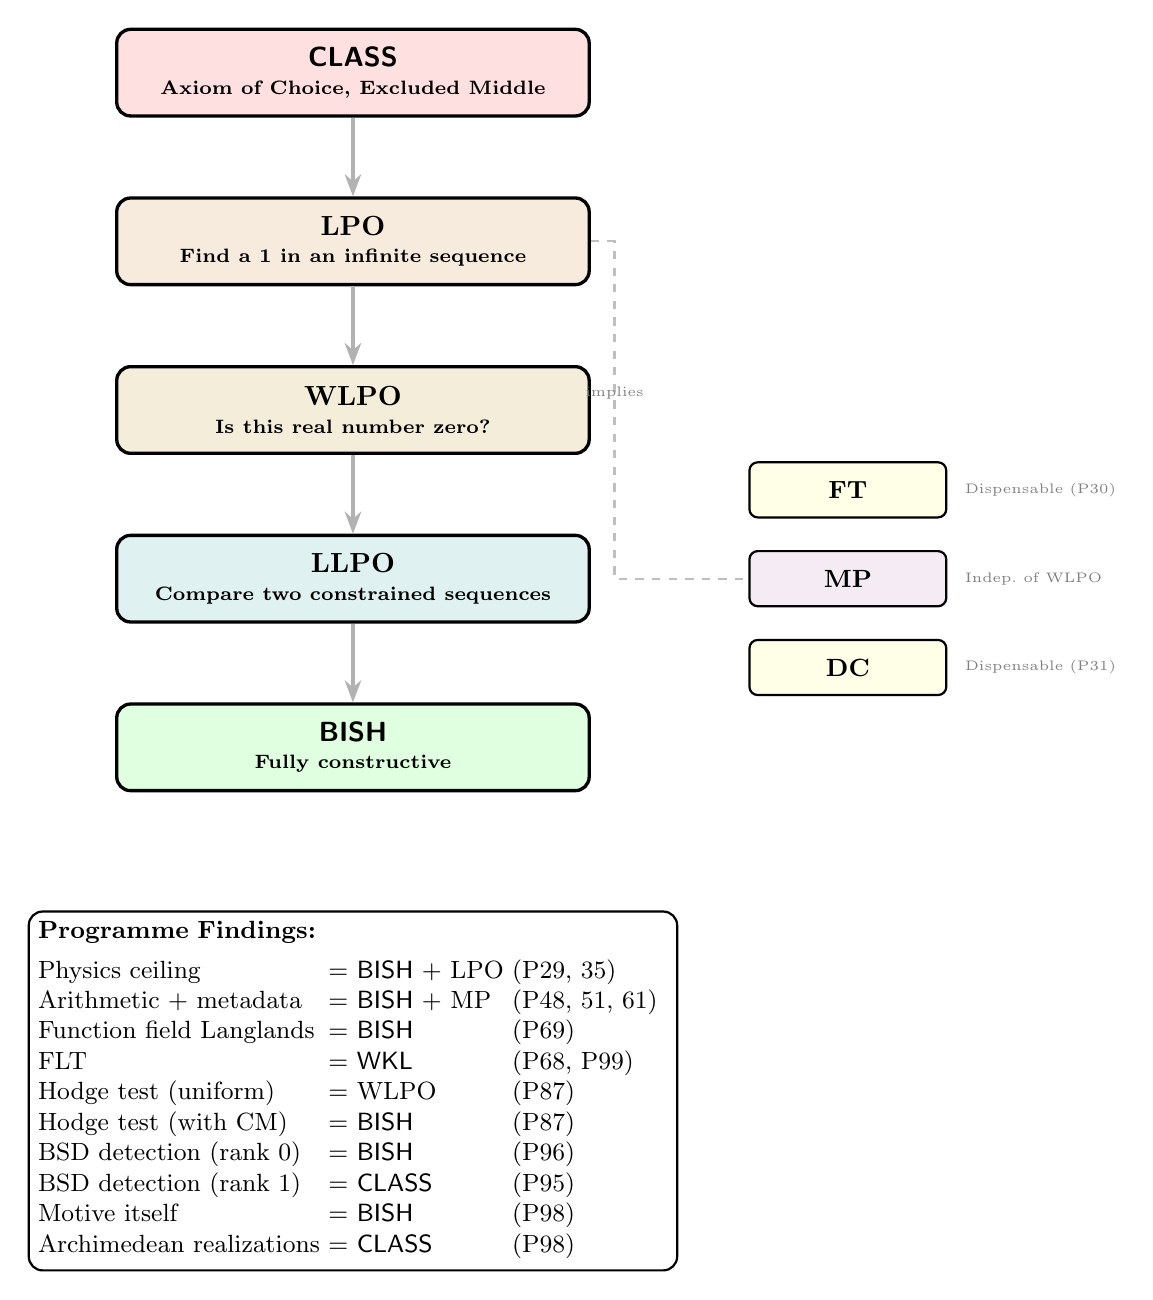
\begin{tikzpicture}[
  level/.style={draw, very thick, rounded corners=5pt,
    minimum width=6cm, minimum height=1.1cm,
    align=center, font=\normalsize\bfseries},
  node distance=1cm,
  implabel/.style={font=\scriptsize, text=gray!70!black, align=left, text width=3.5cm}
]
  % Main spine
  \node[level, fill=red!12] (class)
    {\CLASS\\[-2pt]{\scriptsize Axiom of Choice, Excluded Middle}};
  \node[level, fill=lpoamber!15, below=of class] (lpo)
    {LPO\\[-2pt]{\scriptsize Find a 1 in an infinite sequence}};
  \node[level, fill=wlpogold!15, below=of lpo] (wlpo)
    {WLPO\\[-2pt]{\scriptsize Is this real number zero?}};
  \node[level, fill=llpocyan!12, below=of wlpo] (llpo)
    {LLPO\\[-2pt]{\scriptsize Compare two constrained sequences}};
  \node[level, fill=green!12, below=of llpo] (bish)
    {\BISH\\[-2pt]{\scriptsize Fully constructive}};

  % Arrows on spine
  \foreach \a/\b in {class/lpo, lpo/wlpo, wlpo/llpo, llpo/bish} {
    \draw[very thick, -{Stealth[length=8pt]}, gray!60] (\a) -- (\b);
  }

  % Orthogonal principles
  \node[draw, thick, rounded corners=3pt, fill=mppurple!8,
        minimum width=2.5cm, minimum height=0.7cm,
        font=\small\bfseries, right=2cm of llpo] (mp)
    {MP};
  \node[draw, thick, rounded corners=3pt, fill=yellow!10,
        minimum width=2.5cm, minimum height=0.7cm,
        font=\small\bfseries, above=0.4cm of mp] (ft)
    {FT};
  \node[draw, thick, rounded corners=3pt, fill=yellow!10,
        minimum width=2.5cm, minimum height=0.7cm,
        font=\small\bfseries, below=0.4cm of mp] (dc)
    {DC};

  \draw[thick, dashed, gray!50] (lpo.east) -- ++(0.3, 0) |- (mp.west)
    node[pos=0.25, above, font=\tiny, text=gray] {implies};
  \node[font=\tiny, text=gray, right=0.1cm of mp]
    {Indep.\ of WLPO};
  \node[font=\tiny, text=gray, right=0.1cm of ft]
    {Dispensable (P30)};
  \node[font=\tiny, text=gray, right=0.1cm of dc]
    {Dispensable (P31)};

  % Programme findings
  \node[draw, thick, rounded corners=5pt, fill=white,
        text width=8cm, align=left, font=\small,
        below=1.5cm of bish] (findings) {%
    \textbf{Programme Findings:}\\[4pt]
    \begin{tabular}{@{}l @{\ =\ } l @{\ } l@{}}
    Physics ceiling & \BISH{} + LPO & (P29, 35) \\
    Arithmetic + metadata & \BISH{} + MP & (P48, 51, 61) \\
    Function field Langlands & \BISH & (P69) \\
    FLT & \WKL & (P68, P99) \\
    Hodge test (uniform) & WLPO & (P87) \\
    Hodge test (with CM) & \BISH & (P87) \\
    BSD detection (rank 0) & \BISH & (P96) \\
    BSD detection (rank 1) & \CLASS & (P95) \\
    Motive itself & \BISH & (P98) \\
    Archimedean realizations & \CLASS & (P98) \\
    \end{tabular}
  };
\end{tikzpicture}%
}% end resizebox
\caption{The complete CRM hierarchy with program findings. Each floor strictly implies those below. FT and DC are physically dispensable.}
\label{fig:full-hierarchy}
\end{figure}


%── Appendix D ──────────────────────────────────────────
\chapter{Research Frontiers}\label{app:frontiers}

\begin{analogybox}[What Comes Next?]
A geological survey does not end with the map. Once you know where the hard rock is and where the soft ground lies, you know where to build tunnels---and where tunnels are impossible. The CRM program has produced the map. This appendix identifies the tunnels: specific mathematical targets where the Archimedean Obstruction Thesis makes falsifiable predictions about what cheaper proofs should look like.

Each target below is a \textbf{prediction}: either the theorem can be proved at the predicted CRM level (confirming the thesis), or it cannot (revealing a new obstruction beyond the Archimedean place). Either outcome advances mathematics.
\end{analogybox}


%── D.1 ────────────────────────────────────────────────
\section{Constructive $p$-adic Langlands}

\begin{analogybox}[The Neighbourhood with Its Own Generator]
The $p$-adic Langlands correspondence (Breuil, Colmez, Emerton) is the number-theoretic neighbourhood that never connects to the municipal grid. It matches $p$-adic Galois representations with $p$-adic Banach space representations of $\GL_2(\mathbb{Q}_p)$---\emph{everything stays $p$-adic}. No real integration, no spectral theory on $\mathbb{R}$, no Archimedean place.

It is as if an entire district of the city built its own solar farm and disconnected from the power plant entirely.
\end{analogybox}

\textbf{Prediction.} The $p$-adic Langlands correspondence should be $\BISH + \textsf{WKL}_0$ (WKL for inverse limits in Banach space completions). No \CLASS{} content should arise. A CRMLint Squeeze of Colmez's proof would be a natural future test of the Archimedean Thesis.

\textbf{Why it matters.} If confirmed, this would be the strongest evidence yet that the Archimedean place is the \emph{sole} source of classical content: even the deepest representation-theoretic correspondence is constructive when $\mathbb{R}$ is absent.


%── D.2 ────────────────────────────────────────────────
\section{Condensed Mathematics as a New Lens}

\begin{analogybox}[A Better Microscope]
Scholze's condensed mathematics replaces messy topological spaces with clean algebraic objects (condensed sets = sheaves on profinite sets). In our lens-and-motive language, this is a \emph{brand new realization functor}---a seventh lens for reading the motive's DNA.

The exciting question: does this new lens avoid the Archimedean place? If condensed cohomology can substitute for Betti cohomology in the comparison isomorphisms, it would be like replacing the UV light (expensive, \CLASS) with a new wavelength that reads the same information at the cost of ordinary visible light (\BISH).
\end{analogybox}

\textbf{Obstacle (identified in \paperref{98}).} Full condensed mathematics does \emph{not} avoid \CLASS. The category of condensed abelian groups has enough projectives because extremally disconnected spaces are projective in compact Hausdorff spaces (Gleason's theorem). Gleason's theorem requires the Boolean Prime Ideal Theorem (BPI). BPI is strictly weaker than the full Axiom of Choice, but still non-constructive---it is equivalent to the ultrafilter lemma, which asserts the existence of ultrafilters without constructing them. For the condensed mathematics application, BPI suffices to produce enough projectives, but it remains \CLASS. Condensed mathematics trades \emph{analytic} \CLASS{} axioms (real integration) for \emph{set-theoretic} \CLASS{} axioms (infinite choice). The CRM cost is not reduced.

\textbf{The fix: light condensed sets.} Clausen--Scholze's \emph{light} condensed sets---sheaves on totally disconnected spaces of countable cofinality---avoid Gleason's theorem entirely. The residual cost is sequential completions, which require $\textsf{WKL}_0$ (compactness for inverse limits) or $\textsf{DC}$ (dependent choice for sequential constructions). Since $\textsf{WKL}_0$ and $\textsf{DC}$ are independent over \BISH, determining which governs light condensed cohomology is itself a CRM question.

\textbf{Revised prediction.} Light condensed de Rham $\to$ light condensed Betti has cost $\BISH + \textsf{WKL}_0/\textsf{DC}$, strictly below the \CLASS{} cost of the classical comparison. The Conservation Conjecture (\paperref{67}) becomes testable: is this residual cost optimal?


%── D.3 ────────────────────────────────────────────────
\section{Motivic Iwasawa Theory}

\begin{analogybox}[The $p$-adic Shortcut to BSD]
Recall from Chapter~6 that BSD's classical bottleneck is the Archimedean $L$-function $L(E,s)$, defined by a Mellin transform over $\mathbb{R}$. But there is a $p$-adic version of the $L$-function that avoids $\mathbb{R}$ entirely. Iwasawa theory studies this $p$-adic analogue.

Imagine the BSD question (``does this curve have rational points?'') as asking ``how tall is this building?'' The classical approach measures it from a hilltop across town (looking through $\mathbb{R}$). Iwasawa theory measures it from the basement ($p$-adic, staying inside the building). If the basement measurement is enough, the hilltop trip is unnecessary.
\end{analogybox}

\textbf{Prediction.} $\BISH + \textsf{WKL}_0$ for the algebraic side of the Iwasawa Main Conjecture. The \CLASS{} content enters only through the \emph{interpolation step}---constructing the $p$-adic $L$-function by interpolating complex $L$-values. A purely $p$-adic formulation of BSD that avoids complex $L$-values entirely could achieve $\BISH + \textsf{WKL}_0$.

\textbf{Evidence.} Paper 96's rank-0 test case ($11\mathrm{a}1$, $w = +1$) is suggestive: the modular symbol ratio $L(E,1)/\Omega^+$ is already algebraic (\BISH{} by \texttt{norm\_num}).


%── D.4 ────────────────────────────────────────────────
\section{Trace Formula Excision}

\begin{analogybox}[Replacing the Factory's Assembly Line]
The Arthur--Selberg trace formula is the \emph{universal} \CLASS{} bottleneck. It is the assembly line at the $\mathbb{R}$ power plant: every automorphic result passes through it. The bottleneck is the spectral decomposition of $L^2(G(\mathbb{Q}) \backslash G(\mathbb{A}))$ at the Archimedean place $G(\mathbb{R})$.

Over function fields, this problem vanishes: the geometric trace formula (Frenkel--Langlands--Ng\^o) replaces spectral analysis with the Hitchin fibration. It is as if the factory replaced its diesel-powered assembly line with a solar-powered one.

Over number fields, no such replacement exists. The Archimedean places are structurally required. Finding an algebraic bypass would be the mathematical equivalent of room-temperature superconductivity: extremely valuable, widely sought, and currently beyond known techniques.
\end{analogybox}

\textbf{Assessment: irreducible \CLASS{} (\paperref{98}).} Over number fields, the ``base curve'' is $\mathrm{Spec}(\mathcal{O}_K) \cup \{\infty\}$, and the Archimedean places $\{\infty\}$ are structurally required by Arakelov geometry to compactify the arithmetic curve. There is no purely algebraic ``arithmetic Hitchin fibration'' that ignores infinity. The global trace formula over $\mathbb{Q}$ is an irreducible \CLASS{} node.

\textbf{The local avenue.} The Fargues--Scholze geometrization of the \emph{local} Langlands correspondence uses the Fargues--Fontaine curve (purely $p$-adic, no Archimedean place). This achieves $\BISH + \textsf{WKL}_0$ for local results, but does not excise the Archimedean place from \emph{global} automorphic arguments.


%── D.5 ────────────────────────────────────────────────
\section{Higher-Dimensional Hodge Bifurcations}

\begin{analogybox}[From One Dial to Many]
The palindromic bifurcation in Chapter~5 worked because the genus-4 family had three tuning dials $(a,b,c)$---enough room for a symmetry locus $\{a = c\}$ of dimension 2. Elliptic curves (Chapter~6) had only one dial ($j$-invariant), so no bifurcation was possible.

What about mathematical objects with \emph{more} dials? Higher-dimensional varieties have larger moduli spaces, which means more room for symmetry subloci. The prediction: wherever there are enough dials, constructive Hodge loci should exist.
\end{analogybox}

Three concrete targets:
\begin{itemize}
  \item \textbf{Abelian varieties of dimension $g$:} Moduli dimension $g(g+1)/2$. For $g \geq 3$, positive-dimensional symmetry loci should exist, supporting constructive Hodge class detection.
  \item \textbf{Calabi-Yau threefolds:} The mirror quintic (\paperref{94}) has 1 modulus ($\psi$). But the full quintic family has $h^{2,1} = 101$ moduli. Palindromic-type loci in 101-dimensional moduli are plausible targets.
  \item \textbf{K3 surfaces:} Moduli dimension 20. The Kuga--Satake construction (\paperref{55}) provides algebraic metadata analogous to CM. The Kuga--Satake locus should support a Hodge bifurcation.
\end{itemize}


%── D.6 ────────────────────────────────────────────────
\section{Explicit Langlands Beyond $\GL_2$}

\begin{analogybox}[Scaling Up the Translation Manual]
Paper 78 found that the local Langlands correspondence for $\GL_2(\mathbb{Q}_2)$ is \BISH---the character-trace matching is pure algebra. The global correspondence, by contrast, requires the trace formula (\CLASS).

Think of it as a translation dictionary between two languages. The local dictionary (one city's dialect) can be written by hand (\BISH). The global dictionary (all dialects everywhere) requires a massive statistical survey (\CLASS, via the trace formula).

Can the hand-written approach scale to $\GL_n$? The local data is still algebraic (Bernstein--Zelevinsky classification, Bushnell--Kutzko types). The Archimedean Thesis predicts: \BISH{} for local $\GL_n$.
\end{analogybox}

\textbf{Prediction.} The local Langlands correspondence for $\GL_n$ over $p$-adic fields is \BISH. The \CLASS{} content enters only through the global correspondence (trace formula). A CRMLint Squeeze of the Harris--Taylor proof for $\GL_n$ would quantify the \CLASS{} content precisely.


%── D.7 ────────────────────────────────────────────────
\section{Opportunity Summary}

\begin{table}[htbp]
\centering\small
\renewcommand{\arraystretch}{1.2}
\begin{tabular}{@{}p{3.5cm} l l p{3.2cm}@{}}
\toprule
\textbf{Target} & \textbf{Current} & \textbf{Predicted} & \textbf{Method} \\
\midrule
$p$-adic Langlands (Colmez) & Unaudited & $\BISH + \textsf{WKL}_0$ & CRMLint Squeeze \\
Condensed comparison & Unaudited & $\leq \CLASS$ & Conservation test \\
$p$-adic BSD ($\mathbb{Z}_p$-ext.) & \CLASS & $\BISH + \textsf{WKL}_0$ & Avoid complex $L$-values \\
Trace formula excision & \CLASS & $\textsf{WKL}_0$ & Hitchin bypass \\
CY3 Hodge ($h^{2,1}=101$) & \CLASS & Bifurcation & Palindromic loci \\
K3 Kuga--Satake & \CLASS & Bifurcation & Algebraic metadata \\
$\GL_n$ local Langlands & \CLASS & \BISH{} (local) & Bushnell--Kutzko \\
\bottomrule
\end{tabular}
\caption{Research targets identified by the Archimedean Obstruction Thesis (\paperref{98}). ``Current'' is the CRM cost of existing proofs; ``predicted'' is the framework's prediction for the optimal achievable cost. Each is a falsifiable prediction.}
\label{tab:opportunities}
\end{table}

\begin{thesisbox}[From Catalogue to Predictions]
The motivic CRM architecture transforms the program from a catalogue of individual results into a \textbf{predictive theory}. Each entry in Table~\ref{tab:opportunities} is falsifiable: either the target theorem can be proved at the predicted level (confirming the Archimedean Thesis), or it cannot (revealing a new obstruction beyond the Archimedean place). Either outcome advances mathematics.
\end{thesisbox}


%── Appendix E ──────────────────────────────────────────
\chapter{Controversies Resolved}\label{app:controversies}

The motivic framework from \paperref{98} resolves several issues that arose during the program.

\section{\texttt{Classical.choice} in $\mathbb{R}$-Theorems}

\textbf{The confusion.} Every Lean theorem mentioning $\mathbb{R}$ shows \texttt{Classical.choice} in \texttt{\#print axioms}, even proofs using only \texttt{ring} or \texttt{norm\_num}. Does this mean they are not constructive?

\textbf{The resolution.} No. \texttt{Classical.choice} is a \emph{Lean infrastructure artifact}: Mathlib's construction of $\mathbb{R}$ (Cauchy completion, quotient field, decidable equality on supports) injects this axiom into the type signature. A theorem proved by \texttt{ring} operates in the de Rham realization (algebraic polynomial identity): it is \BISH{} regardless of what the axiom checker reports.

\begin{analogybox}[Analogy: The Factory Stamp]
Every product shipped from a factory carries the factory's quality stamp, even products that never went through the quality testing line. The stamp (\texttt{Classical.choice}) is on the package because the \emph{packaging material} ($\mathbb{R}$ as defined in Mathlib) comes from the factory. The product inside (the polynomial identity proved by \texttt{ring}) was assembled entirely by hand.
\end{analogybox}

\textbf{The principle.} CRM classification is determined by \emph{proof content} (which realization functors and comparison isomorphisms are used), not by the Lean axiom checker output.


\section{DPT vs.\ Fargues--Scholze: Complementary, Not Competing}

\textbf{The confusion.} The DPT axiom scheme (\paperref{50--53, 72--74}) and the Fargues--Scholze geometrization appear to address similar problems. Are they competing frameworks?

\textbf{The resolution.} They are complementary and \emph{logically forced} to partition along the Archimedean boundary:
\begin{itemize}
  \item \textbf{DPT} operates on the Archimedean side: it provides algebraic oracles (Conjecture D, algebraic spectrum, Archimedean polarization) that bypass the three Archimedean comparison isomorphisms.
  \item \textbf{Fargues--Scholze} operates on the non-Archimedean side: it works entirely within $p$-adic Hodge theory, diamonds, and perfectoid spaces---avoiding $\mathbb{R}$ entirely.
\end{itemize}

However, Fargues--Scholze does not achieve \BISH{} for free. It trades the analytic cost of $\mathbb{R}$ for the topological cost of non-Archimedean completeness (completing $\overline{\mathbb{Q}_p}$ to $\mathbb{C}_p$, functional analysis on $p$-adic Banach spaces). This requires $\textsf{WKL}_0$ for compactness and completions. The Archimedean \CLASS{} is eliminated, but a $\textsf{WKL}_0$ residue remains.


\section{FLT vs.\ BSD: Why Their CRM Profiles Diverge}

\textbf{The puzzle.} Both FLT and BSD concern elliptic curves over $\mathbb{Q}$, yet their CRM profiles are qualitatively different. FLT has an enormous \BISH{} core with a single irreducible \WKL{} node (TW patching, \S\ref{sec:flt}); BSD is structurally \CLASS{} with classical content distributed across multiple components (\paperref{95--96}).

\textbf{The explanation.}
\begin{itemize}
  \item \textbf{FLT} asserts \emph{non-existence}: the proof proceeds by contradiction (Ribet level-lowering to $N = 2$, no such form exists). The argument from Frey curve to contradiction routes through \'etale and crystalline realizations (\BISH), with the sole non-constructive content in Taylor--Wiles patching (\WKL: inverse limit of finite local rings). The dihedral base case is \BISH{} (\paperref{99}).
  \item \textbf{BSD} asserts an \emph{equality}: $\mathrm{ord}_{s=1} L(E,s) = \mathrm{rk}\, E(\mathbb{Q})$. The $L$-function uses the Mellin transform at the Archimedean place. \CLASS{} content is \emph{distributed} across the analytic side (the $L$-function \emph{is} the Archimedean realization) and the Galois-cohomological side (Kolyvagin's Euler system requires Chebotarev density).
\end{itemize}

The structural difference: for FLT, the non-constructive content is \emph{concentrated in a single \WKL{} node} (TW patching); for BSD, the \CLASS{} content is \emph{distributed and structural}. This explains why \paperref{96} found no bifurcation for BSD: there is no single node to excise.


\section{Hodge Bifurcation vs.\ BSD Rigidity}

\textbf{The puzzle.} The Hodge conjecture admits a constructive/classical bifurcation (palindromic locus, \paperref{86--89}). BSD does not (\paperref{96}). Why?

\textbf{The explanation.} Bifurcation requires two ingredients:
\begin{enumerate}
  \item A continuous family of mathematical objects (moduli space of dimension $\geq 2$).
  \item A positive-dimensional sublocus where extra symmetry provides an algebraic bypass.
\end{enumerate}

For Hodge: the universal hyperelliptic family has 3 parameters $(a,b,c)$, and the palindromic locus $\{a = c\}$ has dimension 2. For BSD: the moduli of elliptic curves is the $j$-line (dimension 1), and proper algebraic subvarieties are isolated points (CM curves).

\begin{analogybox}[The Highway vs.\ the Path]
As we said in Chapter~6: the Hodge family lives on a multi-lane highway (9-dimensional moduli for genus-4 Jacobians), so there is room for a ``constructive lane'' (the palindromic locus). Elliptic curves live on a single-track path ($j$-line, dimension 1). There is no room for a constructive lane---you are either on the path or off it.
\end{analogybox}


\vfill
\chapter{Logos: Philosophical Foundations}\label{app:logos}

\begin{center}
\foreignlanguage{greek}{%
>En >arq\~h| \~hn <o L'ogos,\\[4pt]
ka`i <o L'ogos \~hn pr`os t`on Je'on,\\[4pt]
ka`i Je`os \~hn <o L'ogos.%
}\\[12pt]
\textit{In the beginning was the Word, and the Word was with God, and the Word was God.}\\[4pt]
--- John 1:1
\end{center}

\vspace{0.5cm}

\noindent The author's original motivation for this program was a search for \foreignlanguage{greek}{L'ogos}---rational structure at the foundations of physics and mathematics. That commitment is recorded in the epigraph and in Paper~40. This appendix sets the program's findings in the context of current debates in the philosophy of mathematics and physics, and explains how CRM addresses open questions that the field's leading thinkers have identified.

\section{The Open Questions in Foundations}

The foundations of mathematics and physics are, as of 2026, in a state of productive tension. Several distinct research programs offer competing or complementary views of what mathematics \emph{is}, what physics \emph{needs} from it, and whether the logical framework matters. The key positions:

\textbf{Wigner's unreasonable effectiveness.}
Eugene Wigner's 1960 observation---that mathematics is ``unreasonably effective'' in the natural sciences---remains unexplained. Why should abstract structures invented by pure mathematicians turn out to describe the physical world? Wigner offered no mechanism. The question has been sharpened but not resolved.

\textbf{Penrose's mathematical Platonism.}
Roger Penrose (2004) argues for a three-world picture: a mathematical world (Platonic), a physical world, and a mental world, with mysterious connections between them. The physical world appears to obey mathematical laws, but Penrose emphasizes that we lack an explanation for \emph{which} mathematics is physically relevant. His tilting toward non-computability (via G\"odel--Turing arguments about consciousness) places him in tension with constructive approaches, yet his insistence that mathematics has objective structure aligns with what CRM discovers.

\textbf{Tegmark's mathematical universe.}
Max Tegmark (2008, 2014) radicalizes Wigner: the physical world does not merely \emph{use} mathematics---it \emph{is} a mathematical structure. The Mathematical Universe Hypothesis (MUH) implies that all consistent mathematical structures are equally real. CRM provides a concrete objection: not all logical frameworks are equally useful for physics. The physical world selects \BISH{} + \LPO{} with perfect precision, not the full classical hierarchy. If the universe is a mathematical structure, it is a very specific one, and the specificity is measurable.

\textbf{Voevodsky's univalent foundations.}
Vladimir Voevodsky (Fields Medal, 2002) spent his final years developing Homotopy Type Theory (HoTT) as an alternative foundation for mathematics, motivated partly by his own experience of errors in published proofs. His program shares two convictions with CRM: (1)~formal verification matters, and (2)~the choice of logical foundation is not neutral. HoTT replaces set theory with type theory and treats equality as a homotopical concept. CRM is orthogonal: it does not change the foundation but \emph{measures} the logical cost within the existing one. The two programs are complementary---HoTT asks ``what foundation should we use?''; CRM asks ``what does the current foundation actually cost?''

\textbf{Feferman's predicativism.}
Solomon Feferman (1998, 2005) argued that all ``scientifically applicable'' mathematics is predicatively reducible---roughly, that physics never needs the full power of set theory. This is close in spirit to what CRM finds, but with a crucial difference. Feferman's criterion is predicativity (avoidance of impredicative definitions). CRM's criterion is constructivity (avoidance of omniscience principles). The two notions overlap but do not coincide: impredicative definitions can be constructive (as in Lean's \texttt{Prop} universe), and predicative mathematics can be non-constructive (classical arithmetic is predicative but uses LEM). CRM provides the finer instrument.

\textbf{Connes's noncommutative geometry.}
Alain Connes (Fields Medal, 1982) has argued that noncommutative geometry reveals the ``fine structure'' of spacetime at the Planck scale. His spectral approach to geometry replaces point-set topology with operator algebras. The spectral theorem---the engine of Connes's entire program---costs exactly \LPO{} in CRM (\paperref{2}). This is not a criticism of Connes but a calibration: his program lives at the physics ceiling (\BISH{} + \LPO), and the non-constructive content enters precisely where he crosses from algebra to analysis (the spectral decomposition of unbounded operators on $\mathbb{R}$).

\textbf{Scholze's condensed mathematics.}
Peter Scholze (Fields Medal, 2018) and Dustin Clausen developed condensed mathematics to repair the categorical deficiencies of classical topology. Their framework replaces topological spaces with condensed sets (sheaves on profinite sets). As discussed in \S3.6 and Appendix~D, condensed mathematics and CRM govern complementary territories: Scholze's framework controls the $p$-adic/geometric sector; CRM controls the algebraic/Archimedean sector. The conservation conjecture---whether \CLASS{} scaffolding in condensed proofs is eliminable---is the open interface.

\textbf{Maddy's naturalism.}
Penelope Maddy (1997, 2011) argues that mathematical methodology should be judged by \emph{mathematical} standards, not philosophical ones. The working mathematician does not need a foundational justification to use the axiom of choice. CRM agrees with the methodological point but adds an empirical one: even if mathematicians do not \emph{need} to justify their axioms philosophically, they can \emph{measure} the logical cost of each axiom empirically, and the measurement reveals structure invisible to both philosophical argument and mathematical practice.

\section{What CRM Contributes}

The program addresses these debates by providing something none of them had: \textbf{empirical data on logical cost at scale}.

\textbf{Against logical arbitrariness.}
The strongest finding is negative: the logical structure of mathematics is \emph{not} arbitrary. If theorems required random assortments of logical principles, CRM would have found a scattered, incoherent map. Instead, it found that all non-constructive content in both physics and arithmetic geometry traces to a single source ($\mathbb{R}$), concentrates at a single mechanism (comparison isomorphisms through the Archimedean place), and is classified by a single hierarchy (Bishop's). This is evidence that the logical structure of mathematics has objective content---supporting Penrose's Platonism, refining Tegmark's MUH, and extending Feferman's predicativism to a finer resolution.

\textbf{A mechanism for Wigner.}
CRM offers a partial explanation for unreasonable effectiveness: mathematics is effective in physics because \emph{physics uses very little of it}. The physics ceiling is \BISH{} + \LPO---constructive mathematics plus one omniscience principle. The vast majority of classical mathematics (\CLASS) is scaffolding that physics never touches. What Wigner observed as ``unreasonable effectiveness'' is partly an artifact of not having measured logical cost: mathematics \emph{seems} unreasonably powerful because we attribute to physics the full cost of \CLASS, when physics only uses the first two floors.

\textbf{Calibration for formal verification.}
Voevodsky's vision of machine-checked mathematics is now reality (Lean, Coq, Isabelle, Agda). But formal verification so far has focused on \emph{correctness} (is the proof valid?) rather than \emph{cost} (what axioms does the proof need?). CRM adds the cost dimension. The 96,200 lines of Lean code in this series are not just verified proofs---they are verified \emph{calibrations}, each tagged with its exact position in Bishop's hierarchy. This provides a template for what large-scale formal verification could become: not just a certificate of truth, but a map of logical dependencies.

\textbf{Constructivity as empirical hypothesis.}
Feferman conjectured that all scientifically applicable mathematics is predicatively reducible. CRM tests and refines a parallel conjecture: all \emph{empirically testable} physics is constructive up to \LPO. Across 42 papers and every major domain of physics---QED, QCD, general relativity, statistical mechanics, quantum information, the cosmological constant problem---the ceiling holds. This is no longer a philosophical position; it is an empirical finding, verified line by line in Lean.

\textbf{The Archimedean thesis as organizing principle.}
None of the programs above---Penrose, Tegmark, Voevodsky, Feferman, Connes, Scholze, Maddy---identified $\mathbb{R}$ as the single source of logical cost. CRM did. The Archimedean Obstruction Thesis (\S1.5) states: non-constructive content enters if and only if the proof path passes through the Archimedean place. This gives the debates a focal point. Instead of arguing in the abstract about whether classical logic is ``necessary,'' one can now ask: does this specific theorem cross the Archimedean boundary? If yes, classical content is expected. If no, look for a constructive proof.

\section{The Author's Motivation}

The Greek word \foreignlanguage{greek}{L'ogos}---word, reason, proportion, account---is what motivated this program. The author went looking for rational structure at the foundations of physics and mathematics, believing it was there to be found. The 98 papers and 96,200 lines of Lean code are what he found. The reader is free to interpret the finding as evidence for mathematical Platonism, as a contribution to the Wigner problem, as a refinement of Feferman's predicativism, or as confirmation of John 1:1. The proofs do not depend on the interpretation.

\vspace{1cm}

\begin{center}
\rule{0.4\textwidth}{0.5pt}\\[8pt]
{\small This monograph covers Papers 1--98 of the Constructive Reverse Mathematics Series\\
by Paul Chun-Kit Lee (NYU).\\[4pt]
All claims are backed by machine-checked proofs in Lean 4 (96,200+ lines, zero \texttt{sorry}).\\
All papers are published with DOIs on Zenodo.\\[4pt]
Series DOI: \texttt{10.5281/zenodo.17054050}}
\end{center}


\end{document}
